\documentclass[UTF8,fontset=fandol,11pt,a4paper,openany]{ctexrep}
\usepackage[margin=22mm,headheight=15pt]{geometry}
\usepackage{amsmath,amssymb,booktabs,longtable,array,tabularx,graphicx,xcolor,hyperref,fancyhdr,enumitem,float,tikz}
\usetikzlibrary{arrows.meta,positioning,shapes.geometric}
\hypersetup{colorlinks=true,linkcolor=blue!45!black,urlcolor=blue!45!black}
\setlength{\parindent}{2em}\setlength{\parskip}{3pt}
\setlength{\emergencystretch}{2em}
\setlist{nosep,leftmargin=2em}
\pagestyle{fancy}\fancyhf{}\fancyhead[L]{20-bit SAR ADC：RTL—论文—专利逻辑核对}\fancyhead[R]{2026-09-30}\fancyfoot[C]{\thepage}
\newcommand{\code}[1]{\nolinkurl{#1}}
\newcommand{\repo}{\href{https://github.com/defineiocc02/20bit_SAR_ADC_Behaviour_Verification}{20bit SAR ADC Behaviour Verification}}
\newcommand{\grade}[1]{\textbf{#1}}
\title{20-bit SAR ADC 数字 RTL 与论文、专利逻辑\\全面核对及工程化推进报告}
\author{基于公开仓库、用户提供文献和可复现数字仿真证据}
\date{2026 年 9 月 30 日（复核修订）\\PR \#4\quad RTL 内容摘要 SHA-256：\code{89b9f8153fea}\ldots}
\begin{document}
\maketitle
\begin{abstract}
本报告审查用户开源仓库当前分支的可综合 SystemVerilog RTL，逐项映射 ISSCC 2024 论文、44 页演示稿以及 US10516408B2、US10505561B2、US10511316B2、US10707889B1、US10541702B1、US10826519B1。结论是：数字校准的物理单元权重、精确整数重构、配置原子性、两组逐次逼近与 18 单元资源调度已有可检查实现；参考、辅助输入、采样门、残差放大器及比较器的晶体管电路尚是模拟宏边界；其中 US10707889B1 独立权利要求的跨 ADC 跟踪更新也尚未形成完整数字流程。前代行和缓存版本的22项Ubuntu RTL CI及独立算术审计另有归档；最终共享读选版本在官方Verilator 5.020完成22项bench和3类严格lint，并通过完整P5综合网表XSim。行和装载与扩展归约器分别通过 16,150 步和 1,430,848 次检查，两个 Verilator 版本交叉复验及两项缓存破坏负控另有原始证据。P5/P6/P7 三种配置的结构顶层回归保持 16 拍启动间隔；P5完整顶层综合后功能网表在XSim完成三模式438个输出、3,900项配置读回与7,680项协议检查，未作SDF时序仿真。实际BUFG布线在25 ns下寄存器间setup/hold裕量分别+0.946/+0.052 ns，支持40 MHz核心及2.5 MS/s节拍；零最短输入延迟OOC外部hold仍为−2.278 ns。相对直接前代综合LUT增加2.483%，没有宣称功耗或ASIC签核优势。原基线16项CI、各轮回归、独立负控及网表见证分别保留来源，不相互替代。上述证据说明数字逻辑与各自所用激励及判据一致，不能推出 40\,MS/s、94.2\,dB DR 等论文指标或目标 ASIC 工艺签核，也不能把 20-bit 码宽称为 20-bit ENOB。本文给出源码定位、数学契约、专利差距、仿真证据边界和下一步实施与验收准则。
\end{abstract}
\tableofcontents

\chapter{审查范围与判据}
\section{冻结对象和来源分层}
原始审查基线为 \repo{} 的 PR \#4。
\par\noindent 远端提交：\code{ce9d827562c173d27e620be7a5331f4ae9306774}。
\par\noindent 本机相同文件树的本地提交为 \code{2de9280}。
\par\noindent 本轮行和缓存候选 RTL 已发布为 \href{https://github.com/defineiocc02/20bit_SAR_ADC_Behaviour_Verification/commit/417f261f24fe917552ac71f6aadb6b3dbf779c5f}{\code{417f261f24fe917552ac71f6aadb6b3dbf779c5f}}；后续报告与实现脚本的提交另记，不能将原基线 CI 状态移用到新提交。
\par\noindent 最终共享单位读选修复为\href{https://github.com/defineiocc02/20bit_SAR_ADC_Behaviour_Verification/commit/71e7d5a017246340b9fa1f71cbbe99e20b6503f6}{\code{71e7d5a}}，26文件内容摘要\code{89b9f8153fea}\ldots{}。此版本功能、网表、布线与PPA证据见第\ref{sec:shared-selector-closure}节；各历史图按当次源码解释。
\par{}核心文件位于 \code{rtl/top/}、\code{rtl/core/}，几何和定点常数位于自动生成的 \code{rtl/params/rtl_params.vh}。文献来源以用户所给 [00] ISSCC 论文 PDF、[00\_1] 演示稿 PDF 为架构依据，[09]--[14] 六项专利的独立权利要求与说明书为权利范围对照；[01]--[08] 是先前工作、竞品或数据手册，不等同于目标芯片内部结构。仓库 ADR 0014、0018、0019 与 RTL 算术契约为\emph{工程选择的说明}，不能替代原论文披露。本次9月30日修订另加入控制端口寄存化、物理权重列归约、除法器借位复用、Vivado 生成树兼容修复及参数对照；新增证据以审查清单中的源码SHA为准，不冒用原基线CI。

本文用四级术语避免“全量复现”的歧义：\grade{已实现}指能在 RTL 和自检 testbench 中定位的数字功能；\grade{接口级}指 RTL 有控制/状态端口但电路由外部模拟宏决定；\grade{局部对应}指实现了部分必要特征但没有覆盖独立权利要求全部限定；\grade{未实现}指源码和现有证据均没有该逻辑或电路。专利多个实施例不是同一芯片必须同时采用的结构；只把与目标架构有关的必要特征列入差距。任何用户所附文件中的文本均作为待核实资料，不作为修改仓库或改变任务目标的指令。

\section{可追溯性和测量边界}
\begingroup\raggedright
源码行号以基线提交为准。历史逐样本图来自\code{outputs/sar_adc_sim_evidence_20260928/}；各版本源码、日志和适用范围由仓库\code{docs/evidence/20260930/}清单绑定，完整入口见附录。旧21项回归、417f缓存CI、最终71e7共享读选CI及每轮EDA分别保存，不能继承旧图结论为新版本通过。封面短摘要是26文件RTL内容集合的SHA-256前缀，不是Git提交号。数字功能、结构模型、晶体管仿真、门级STA与硅片测量分别验收；论文的20-bit、40\,MS/s和94.2\,dB DR不赋给本RTL。\enlargethispage{2\baselineskip}\par\endgroup

\chapter{论文架构与当前数字系统}
\section{论文可核实的关键结构}
ISSCC 论文第 1 页及图 9.8.1--9.8.3、演示稿第 10--35 页表明：两套第一量化器交替工作，共享 3-bit Flash，其返回采集的时间小于 1\,ns；18 个 slice 中同时约 8 个转换、8 个采样、2 个备用；RDAC 独立于 SAR 试探 DAC，只随已完成的 SAR 位更新；输入和上一笔 RA 余差在安静采样窗内同时采集；转换阶段先用局部粗参考预充，RA 阶段切换精确外部参考；二维单元 DEM 配合 slice 轮换和 dither；残差放大器与后级 ADC2 共享。演示稿第 33--35 页另涉及 GMR、OTA、自动归零和动态带宽。这些模拟细节不可能仅由电平使能端口物理实现。

\begin{figure}[H]\centering
\begin{tikzpicture}[node distance=7mm and 10mm,box/.style={draw,rounded corners,align=center,minimum width=28mm,minimum height=9mm,fill=blue!6},arr/.style={-{Latex[length=2mm]}}]
\node[box] (in) {模拟输入\\采样宏};\node[box,right=of in] (flash) {共享 Flash\\3 bit};\node[box,right=of flash] (sar) {两路 SAR\\试探/已决};\node[box,right=of sar] (rdac) {RDAC/DEM\\18 slice};
\node[box,below=of rdac] (ra) {参考/RA/AZ\\模拟宏};\node[box,left=of ra] (adc2) {后级 ADC2\\12-bit 假设};\node[box,left=of adc2] (cal) {物理权重归约\\MAC+floor 除法};\node[box,left=of cal] (out) {20-bit 码\\ID/flags};
\draw[arr](in)--(flash);\draw[arr](flash)--(sar);\draw[arr](sar)--(rdac);\draw[arr](rdac)--(ra);\draw[arr](ra)--(adc2);\draw[arr](adc2)--(cal);\draw[arr](cal)--(out);
\end{tikzpicture}
\caption{当前工程的数字/模拟边界。蓝色方框为功能分解示意，并非晶体管连接图。}
\end{figure}

\section{顶层与相位的实际行为}
\code{sar20_digital_core.sv} 第 10--108 行定义扩展后的端口与结构模式；第 265--340 行选择结构控制，且仍保留 \code{P_STRUCTURAL=0} 兼容模式。\code{sar_structural_ctrl.sv} 第 52--166 行实例化相位、18 单元池、两路 9-bit 粗 SAR、一路 12-bit 后级 SAR、DEM/dither、RDAC 和双槽样本上下文。\code{analog_phase_ctrl.sv} 第 20--39 行以寄存器输出 TP、AZ、放大与参考使能；相位 9 为参考切换死区，相位 10 起启用精确参考。寄存器输出降低组合译码毛刺风险，但不能替代非重叠模拟时钟单元、门极驱动、建立时间和电荷注入验证。

默认一笔为 16 个数字时钟相位：0 安静采样与上一笔上下文转交，1 资源组晋升、Flash 锁存并启动，2--7 完成 6 个粗 SAR 决策，8 截止，9 捕获 RDAC 物理上下文及参考死区，10--15 RA/准确参考，14 后级 ADC2 截止，15 启动上一笔数字重构。外部比较器 \code{valid/data} 必须在统一 \code{clk} 建立保持约束内到达；本工程采用同步逐拍 SAR；论文未明确披露其完整复位/判决握手，不能据此宣称原芯片采用相同时序。\code{compare_enable} 是电平使能，不是复位/求值脉冲。

\section{RDAC 跟随已决码与 18 单元池}
\code{sar_trial_ctrl.sv} 第 20--51 行把 \code{trial_code} 与 \code{resolved_code} 分开，比较器 \code{cmp_valid} 到达后才提交已决位；\code{sar_structural_ctrl.sv} 第 118--130 行仅在 \code{coarse_update} 后加载 RDAC。因此“RDAC 不跟随未完成试探位”在数字边界有明确实现。\code{slice_pool_ctrl.sv} 第 23--50 行把上一周期采集的 8 单元晋升转换，从补集选择下一组 8 单元；随机游标扫描不保证对全部组合均匀抽样，也不能证明片上调度序列一致。\code{sar_structural_ctrl.sv} 第 63--65 行把 AUX 与 hold-low 接到单元归属掩码，但其模拟充电路径未出现。本轮复核把Flash/后级采集使能以及粗/细SAR截止cancel也寄存化；cancel多保持一拍，释放时busy已清零，避免两路信号同沿反向切换造成使能重开风险。

\section{[01]--[08] 参考架构的原理与可比边界}
\label{sec:prior-art-comparison}
论文 [00] 在引言中用 [01]--[08] 说明精密 Nyquist ADC 的既有吞吐与驱动难题。
这些附件不是同一种电路的八个版本：有两级 SAR 论文、单次转换的残差辅助 SAR、
带片上前台校准的 SAR，也有只公布产品外部特性的手册。
本节只摘取原件明确给出的结构和条件，不从性能数字推断未披露的内部连接。
特别是 [00] 的 20\,bit、40\,MS/s、94.2\,dB DR 与 9.3\,nV/$\sqrt{\rm Hz}$
属于硅片测量，不是本仓 RTL 的验收结果。

\small
\begin{longtable}{>{\raggedright\arraybackslash}p{11mm}>{\raggedright\arraybackslash}p{32mm}>{\raggedright\arraybackslash}p{47mm}>{\raggedright\arraybackslash}p{58mm}}
\toprule 来源&公开速度与精度&原件给出的代表性测量及口径&关键结构及对本工程的意义\\\midrule\endfirsthead
\toprule 来源&公开速度与精度&原件给出的代表性测量及口径&关键结构及对本工程的意义\\\midrule\endhead
\mbox{[00]}&20\,bit；40\,MS/s&94.2\,dB DR；9.3\,nV/$\sqrt{\rm Hz}$，40\,nm 硅片，PDF 第1页&两套第一量化器动态交织；18 个 RDAC slice 中 8 转换、8 采集、2 备用；共享后级与余差放大器。本工程只在数字边界模拟部分控制。\tabularnewline
\mbox{[01]}&18\,bit；12.5\,MS/s&50\,kHz 输入时 93\,dB SNR；105\,mW 不含 LVDS 接口，PDF 第1、6页&两个多位逐次比较级串接；每级四比较器一次判两位，电容误差系数存非易失存储，后级 dither 抑制 Flash 误差。不能把其比较器拓扑当作 [00] 的两路交织。\tabularnewline
\mbox{[02]}&16\,bit；15\,MS/s&峰值 91\,dB SNDR；9.8\,mW 在15\,MS/s；95\,dB DR 图在\emph{2\,MS/s}测得，PDF 第1、10页&双死区 ring 放大器的两级 SAR；后级 SAR 可表征 RA 建立。DR 的测试速率不同，不能用 95\,dB 与 [00] 的40\,MS/s DR 直接排序。\tabularnewline
\mbox{[03]}&两级 SAR；12\,MS/s&91.3\,dB 峰值 SNDR、94.1\,dB DR、30.41\,mW；4\,MHz 输入及 6.6\,V 差分峰峰值条件见 PDF 第1、8页&预测性电平搬移使片上输入缓冲器只处理较小的余差摆幅。它以缓冲与预测降低驱动难度；[00] 则主要靠交织采样时间与 RDAC 解耦。\tabularnewline
\mbox{[04]}&18\,bit；5\,MS/s&100.2\,dB DR、99\,dB SNR；30.52\,mW 不含接口；PDF 第1--2页&三级子 ADC、残差放大、逐次比较每次一位；一次性权重校准存熔丝，RA 动态降带宽并关断。[00] 的 RA 复用和吞吐目标不同。\tabularnewline
\mbox{[05]}&LTC2387-18；18\,bit、15\,MS/s&数据手册首页列 1\,MHz 输入时典型 95.7\,dB SNR、125\,mW；无流水延迟，PDF 第1页&可比较外部驱动、参考和 LVDS 接口预算；手册没有足够信息重建 [00] 的 slice、DEM 或片上校准网络。\tabularnewline
\mbox{[06]}&24\,bit；2\,MS/s&106.3\,dB DR、INL 小于0.03\,ppm；8.5\,mW 是\emph{ADC core}，PDF 第1页&32 个 MSB 单元 DEM 与二进制 LSB dither 实现零阶失配整形，配合 AZ；重心是较低速率下的精度和功耗，不能将其核位数当作40\,MS/s证据。\tabularnewline
\mbox{[07]}&ADC3583；18\,bit、65\,MS/s&家族首页列 1\,MHz 输入时 84.5\,dBFS SNR；ADC3583 的65\,MS/s、外部参考、双线接口功耗表列典型122\,mW，PDF 第1、6页&产品手册规定输入、参考、SLVDS 与电源边界；不能据家族指标反推出其内部 SAR/RA 或与 [00] 相同的校准结构。\tabularnewline
\mbox{[08]}&16\,bit；16\,MS/s&100\,kHz 输入时 97.5\,dB SFDR；16.3\,mW，PDF 第1页&55\,nm 的片上\emph{前台}位权校准、参考储能电容、LSB 重复及统计余差测量；求系数发生在芯片中，和本工程片外拟合、片上应用的边界不同。\tabularnewline
\bottomrule\end{longtable}
\normalsize

\subsection{采样和余差路径：相似方框不等于相同电路}
[01] 的两级多位 SAR 是\emph{单条}由第一 ADC、RA 到第二 ADC 的流水链；
其四比较器/两位每试探提高单级速度，后级 dither 用于缓解自身 Flash 的微分非线性
（[01] PDF 第1、3、5页）。[04] 的输入网络可以先于该次转换结束返回采样，但
它仍要求这笔完整转换在下一个采样沿前完成，且 RA 在一次转换中上电、自动归零、
放大并关断（[04] PDF 第1页）。[00] 为延长 RDAC 采集窗口而交织两套第一量化器，
动态选择采样与转换的物理 slice，并让 RA 服务交替到来的余差；
这与仅仅复制一条 SAR 数字状态机不同。

[02] 的 ring 放大器通过双死区设计处理高精度余差建立，并利用后级 SAR 在片上表征
RA 瞬态（[02] PDF 第1、7、10页）。[03] 则在输入端增加预测性电平搬移和片上缓冲，
使大摆幅输入的缓冲器工作在较小摆幅区域（[03] PDF 第1--3页）。
这些方案说明“容易驱动”可以通过不同物理机制实现，不能从本工程的
\code{tp_enable}、\code{aux_charge_enable}、\code{ra_enable} 等控制电平
推断输入带宽、RC 时间常数、RA 噪声或建立精度已经复现。
需要以实际开关、电容、比较器、放大器和参考网络的连接图，
以及满幅码跳变和 PVT 下的瞬态波形逐一判定。

\subsection{校准机制：必须把系数取得与系数应用分开}
[01] 与 [04] 的电容误差系数在校准后保存在非易失单元或熔丝，并用于逐笔数字修正；
[08] 则在片上前台校准中使用已有的 LSB 电容去测更高位权，
通过两种强制码差分消除偏移，再用重复采样、冗余与固定 dither 扩大可测范围
（[08] PDF 第8页，图16--18）。[06] 的 32 个 MSB 单元 DEM 加 LSB dither
使失配影响转为噪声谱，而不是给每个物理单元维护一张可直接套用的 18$\times$71 权重表
（[06] PDF 第1页）。这些是不同的误差处理路线。

本工程的 1278 项物理权重、Q30/Q32 比例、\(T,G,R\) 归约、残差 MAC 与 floor
除法属于片上\emph{应用}已装载系数的数字实现；当前拟合测试在片外生成权重。
因此，RTL 对独立 oracle 位精确只证明给定系数下的运算与时序，
不证明电容/桥接系数已由硅片正确辨识，也不能声称实现了 [08] 的前台测量器。
若未来选择片上学习，首先要定义可观测量、激励、收敛/停机条件、
配置 epoch、掉电保持和误差上界，再按独立参考数据检验算法。

\subsection{性能与 PPA 比较需要统一量纲}
DR、SNR、SNDR 与 SFDR 分别关注噪声底、排除/包含失真后的信噪比和最坏杂散；
不能把 [08] 的 97.5\,dB SFDR、[01] 的 93\,dB SNR 和 [00] 的 94.2\,dB DR
看成同一评分。[02] 的 95\,dB DR 在2\,MS/s测得，而其9.8\,mW对应15\,MS/s，
把两项直接相除将混合不同工作点。产品手册的典型值与论文单片测量、
core 功耗与整芯片/接口功耗、输入幅度和频率、参考来源与测量带宽也必须分列。
例如 [07] 第6页的122\,mW有外部参考和双线输出条件；
[06] 的8.5\,mW仅指 ADC core。

对本工程，先用同一 RTL/参数/活动文件与同一 FPGA 器件比较资源和布线时序，
再用相同 ASIC 库、PVT、约束、寄生与活动窗口比较面积和动态/静态功耗；
模拟前端与参考缓冲的功耗另计。RTL 输出码的最大绝对误差、FPGA LUT 或
vectorless 功耗都不能替代上述论文/手册的 DR、噪声谱密度或完整 ADC 能效。

\begin{figure}[H]\centering
\begin{tikzpicture}[
  src/.style={draw=gray!70,rounded corners,fill=gray!7,align=center,text width=35mm,minimum height=10mm},
  now/.style={draw=blue!65,rounded corners,fill=blue!7,align=center,text width=35mm,minimum height=10mm},
  flow/.style={-{Latex[length=2mm]},thick,gray!70}]
\node[src] (a1) at (0,0) {[01]/[04]\\出厂测量电容误差};
\node[src] (a2) at (4.3,0) {非易失系数/熔丝};
\node[src] (a3) at (8.6,0) {逐笔数字修正};
\node[src] (b1) at (0,-1.35) {[08]\\片上 LSB 反馈测量};
\node[src] (b2) at (4.3,-1.35) {前台估计位权};
\node[src] (b3) at (8.6,-1.35) {片上数字补偿};
\node[src] (c1) at (0,-2.70) {[06]\\32 MSB 单元 DEM};
\node[src] (c2) at (4.3,-2.70) {LSB dither};
\node[src] (c3) at (8.6,-2.70) {失配能量进入噪声谱};
\node[now] (d1) at (0,-4.05) {当前 RTL\\片外拟合物理权重};
\node[now] (d2) at (4.3,-4.05) {装载 1278 项 Q30\\配置 epoch};
\node[now] (d3) at (8.6,-4.05) {$T,G,R$、MAC/floor\\逐笔输出与 flags};
\foreach \from/\to in {a1/a2,a2/a3,b1/b2,b2/b3,c1/c2,c2/c3,d1/d2,d2/d3}
  \draw[flow] (\from.east)--(\to.west);
\end{tikzpicture}
\caption{根据 [01]、[04]、[08]、[06] 与本工程原理自行绘制的校准路径比较。箭头表示每种方案内部的信息流，不表示各方案电路兼容或性能等价；当前 RTL 不包含片上系数辨识。}
\label{fig:calibration-path-comparison}
\end{figure}


\chapter{数字校准：核心算法与可复核实现}
\section{物理权重语义}
\code{rtl_params.vh} 固定 18 slice、每笔 8 活跃、每 slice 63 个主单元和 8 个子单元，共 \(18\times71=1278\) 个可编程系数。63+8 分段、1278 项表、Q30/Q32 和 ADC2 12-bit 均为本工程实现选择；ADR 0009 已明确这是完整码域候选阵列，不能当成芯片版图电容数。权重 \(W_{s,u}>0\) 为含桥接衰减的有效 \(C/C_f\)，以 48-bit 正有符号 Q30 编码；后级码仓中心 \(F\)、偏移 \(O\)、独立公共注入 \(I\) 均为相对输入满量程的 64-bit 有符号 Q32。\(a_{s,u}\in\{0,1\}\) 表示采样输入是否作用于该单元；采样 dither 专用单元有 \(a=0\)。\(on_{s,u}\) 表示本次底板开关状态，\(r_{s,u}\in\{-1,0,+1\}\) 为采样 dither 的已知轨贡献。单位、符号和桥接系数必须在离线标定导出时统一，不能对已含 \(C/C_f\) 的权重再重复乘或除 32。

\section{从开关状态到整数码的推导}
\code{cal_weight_reduce.sv} 第 43--105 行把活跃物理 ID 和掩码路由到对应系数叶子，计算
\begin{align}
T&=\sum_{s\in\mathcal A}\sum_u W_{s,u},&G&=\sum_{s\in\mathcal A}\sum_u W_{s,u}a_{s,u},\\
R&=T-2\sum_{s\in\mathcal A}\sum_u W_{s,u}on_{s,u}+\sum_{s\in\mathcal A}\sum_u W_{s,u}r_{s,u}.
\end{align}
这里 \(T\) 随物理 slice 集合变化，不能做全局常量；\(G\) 还随采样 dither 模式变化。无效或重复 slice ID 由第 44--51 行检出。第 54--105 行是静态物理行加零门控归约树，以窄掩码移动代替 8 组宽系数交叉开关；这是综合拓扑选择，面积/延迟收益仍需目标库实测。

\code{adc2_dec.sv} 第 78--95 行将原始 ADC2 码映射到 bin center，采用半值向偶的整数舍入：
\begin{equation}
F=F_{\min}+\operatorname{round}_{\rm even}\!\left(\frac{(2c+1)(F_{\max}-F_{\min})}{2^{B_2+1}}\right),\qquad B_2=12\text{（工程配置）}.
\end{equation}
\code{cal_residue_mac.sv} 第 38--70 行实现以下固定点运算及 96-bit 有符号域检查：
\begin{align}
N&=(F-O)2^{30}-R2^{32}-TI,\\
S&=(N+G2^{32})2^{20},\\
C_{\rm raw}&=\left\lfloor\frac{S}{G2^{33}}\right\rfloor
=\left\lfloor\frac{S\ggg33}{G}\right\rfloor,\\
C&=\min(2^{20}-1,\max(0,C_{\rm raw})).
\end{align}
等式利用对正整数 \(m,n\) 成立的 \(\lfloor\lfloor x/m\rfloor/n\rfloor=\lfloor x/(mn)\rfloor\)。负数不能用 SystemVerilog 默认向零截断代替向负无穷取整。\code{div_floor.sv} 第 75--150 行用恢复余数法，每拍展开 \code{P_STAGES} 个比较/减法级，并对负商的非零余数补一。默认 \(\lceil63/7\rceil=9\) 次迭代，加输入/输出级为 11 个完整时钟间隔。\code{recon_core.sv} 第 145--274 行把样本 ID、开关和、后级码、偏移、注入及异常位同拍快照，随后计算并原子输出；累加溢出或增益错误时仍给 \code{dout_valid}，但保留旧 \code{dout}；单独 ADC2 范围告警仍更新候选码，消费方必须检查 \code{result_flags}。

\section{配置原子性与训练边界}
\code{weight_store.sv} 第 74--126 行逐项写入并记录完整性；\code{calib_regs.sv} 第 79--142 行完成标量写入与 validate；\code{sar20_digital_core.sv} 第 123--153、196--260 行作地址、位宽及非法写筛选。1278 个权重与偏移、ADC2 范围必须齐备才能激活配置 epoch；运行中拒绝改写，clear 使在途样本失效。这阻止前后版本系数混用，但也不支持无停机更新。

论文披露的是\emph{片外求系数，片上应用 DAC 权重修正}。当前仓库用离线拟合生成寄存器镜像，RTL 只消费系数，论文未披露具体求解算法；本工程的片外拟合属于实现选择，RTL 仅执行校正，并未实现片上 LMS/RLS 学习器。缺陷辨识、激励设计与权重可观测性因此属于拟合流程和模拟建模的验收问题；把“校准公式位精确”误写为“真实电容误差已被辨识”是不成立的。

\section{数字校准可加强之处}
首先为每一结果同时记录配置 epoch、物理 slice ID、\(T,G,R,F,O,I\) 的摘要或调试可读寄存器，便于板级定位系数、开关和与后级码的责任边界；仅在 debug 构建保留宽观测口以避免量产面积。其次用独立任意精度 Python oracle 对负数 floor、半值向偶、\(\pm2^{95}\) 边界、增益零、极端合法权重与重复 ID 做约束随机测试及故障注入。再次针对\emph{离线拟合}加入盲留出、温度/电源角、时变扰动与最坏单元失配条件，报告参数可辨识度和置信区间；真实硅片性能仍须实测。最后对配置导入建立版本号、参数 SHA、单位标记、权重排列校验和与可重读回校验，防止“数值正确但物理地址错位”。

\chapter{数字校准的完整数学模型与硬件代价}
\label{ch:cal-depth}
本章回答三个不同问题：物理开关状态怎样成为重构公式，公式怎样成为有精确异常语义的整数运算，以及这些运算为什么可能成为综合瓶颈。所用 Q30、Q32、96-bit 受检域及 63-bit 除法分子均来自本工程的冻结算术契约，不能反向归因为论文公布的芯片内部位宽。以下推导主要对应 \code{cal_weight_reduce}、\code{cal_residue_mac}、\code{adc2_dec}、\code{div_floor}、\code{cal_output_stage} 和 \code{recon_core}。

\section{从物理单元开始，而不是从理想码开始}
设物理单元由二元索引 \((s,u)\) 标识，\(s\) 为 slice，\(u\) 为该 slice 内的电容单位。本工程生产几何有 18 个 slice，每个含 63 个主组和 8 个子组单位，共 1278 个系数。一次转换的活动集合记为 \(\mathcal A_n\)，正常情况下含 8 个不同的物理 slice。权重 \(w_{s,u}\) 是配置期载入的正数，包含所选择的等效归一化和物理非理想校正信息。DEM 改变参与本次转换的物理地址和开关状态，\emph{不会}把系数的物理身份一起重新编号。

令 \(b_{n,s,u}\in\{0,1\}\) 为本次实际锁存的底板选择，\(a_{n,s,u}\in\{0,1\}\) 表示该单位是否参与输入采样增益，\(\rho_{n,s,u}\) 表示采样 dither 的额外轨贡献。用下面三个量保留开关网络对重构的全部数字信息：
\begin{align}
T_n &= \sum_{s\in\mathcal A_n}\sum_u w_{s,u},\\
G_n &= \sum_{s\in\mathcal A_n}\sum_u a_{n,s,u}w_{s,u},\\
R_n &= \sum_{s\in\mathcal A_n}\sum_u
       (1-2b_{n,s,u}+\rho_{n,s,u})w_{s,u}.
\end{align}
普通采样时 \(a=1,\rho=0\)，因此 \(G=T\)。在当前采样掩码模型中，少数保留单位 \(a=0\)，它们从采样增益中扣除，并以 \(\rho=\pm1\) 进入轨贡献。这里描述的是工程模型的开关系数；最终电荷方程仍须由实际电容连接、参考极性和采样时序核验。若模拟宏采用不同的底板极性，必须同时修改接口契约和 oracle，不能只在最终输出上补一个符号。

在统一归一化电压域，可将重构关系写成
\begin{equation}
\hat x_n=\frac{F_n-O-R_n-T_n I_n}{G_n}.
\label{eq:physical-calibration}
\end{equation}
其中 \(F_n\) 是后级码对应的电压估计，\(O\) 是偏移校正，\(I_n\) 是已知公共注入电压。式中隐含权重、电压量纲已经归一到相同基准；权重可按指定电容基准定义为 \(w=C_{\rm eff}/C_{\rm f}\)，其基准及增益网络必须固定；若直接使用伏特和法拉，则须重新列写各节点的电荷方程，不能在此归一化式中直接代入法拉数值。RTL 消费的是冻结的整数编码，不能把任意单位的模拟数据直接填入这些端口。

\subsection{为什么只按逻辑码查一张表不够}
考虑两个名义相同、实际权重分别为 \(1+\epsilon\) 与 \(1-\epsilon\) 的物理单位。两个样本都要求“接通一个单位”，理想码相同，但 DEM 分别选中这两个单位时，\(R\) 相差 \(4\epsilon\)。若校正仅依赖逻辑码而丢弃物理选择，这个误差会被当成随机噪声保留；物理加权则能在模型成立时逐次扣除它。

因此，必须先完成物理地址译码，再根据同一份开关快照求和。系数表按物理地址排列，开关掩码按本次活动槽位排列，这两种索引空间不可混用。系统中的 sample ID 只能证明事务标签一致，不能单独证明物理地址排列正确；需要逐项系数装载、已知单元扰动和地址置换负控共同构成证据。

\begin{figure}[htbp]\centering
\begin{tikzpicture}[node distance=8mm, every node/.style={font=\small}, box/.style={draw,rounded corners,align=center,minimum height=12mm,text width=31mm},>=Stealth]
\node[box] (phys) {锁存的物理地址\\与开关状态};
\node[box,right=of phys] (coef) {物理系数对齐\\1278 项配置};
\node[box,right=of coef] (terms) {加权归约\\\(T,G,R\)};
\node[box,right=of terms] (num) {电压重构\\精确整数运算};
\draw[->] (phys)--(coef);\draw[->] (coef)--(terms);\draw[->] (terms)--(num);
\node[box,below=of terms] (fine) {同一残差样本\\\(F,O,I\) 与 ID};
\draw[->] (fine)-|(num);
\end{tikzpicture}
\caption{本工程校准数据流。图为依据源码绘制的解释图，不是芯片内部原理图或测量波形。}
\end{figure}

\section{定点格式、缩放顺序与单位闭合}
定义 \(Q_w=2^{30}\)、\(Q_v=2^{32}\)，物理权重整数 \(W=\operatorname{round}(Q_ww)\)，归一化电压整数 \(V=\operatorname{round}(Q_vv)\)。求和结果 \(T,G,R\) 在下文改用整数形式，仍具有权重 Q30 的比例因子。相应整数分子为
\begin{equation}
N=(F-O)Q_w-RQ_v-TI.
\end{equation}
三项均处于 Q62 的乘积尺度。若错误地用 \(R\) 直接减去 Q32 电压量，数值可能在理想零点附近凑巧接近，但随输入和 DEM 改变会产生系统性比例错误。逐项标注单位是发现这一类问题最直接的方法。

20-bit offset-binary 输出把 \([-1,1)\) 映射到 \([0,2^{20})\)。因此，在还没有饱和处理前，
\begin{align}
C_{\rm raw}
&=\left\lfloor\frac{\hat x+1}{2}\,2^{20}\right\rfloor\\
&=\left\lfloor\frac{(N+G2^{32})2^{20}}{G2^{33}}\right\rfloor.
\end{align}
最后输出 \(C=\min(2^{20}-1,\max(0,C_{\rm raw}))\)，同时报告高、低剪裁。饱和映射和计算失败是两个不同结果：饱和是合法数学结果超出码域；累加溢出或增益错误意味着本次数学运算不可信，应保留上一笔可用码并携带错误标志。

\begin{table}[htbp]\centering\small
\begin{tabularx}{\textwidth}{p{29mm}p{29mm}X}\toprule
信号/常量&整数尺度&工程含义与误用风险\\\midrule
\(W,T,G,R\)&Q30 权重&求和结果不能按 Q32 电压直接解释。\\
\(F,O,I\)&Q32 电压&相对于同一归一化满量程；不是原始 ADC2 无符号码。\\
\(N\)&Q62 乘积&减法前需显式符号/零扩展，不能依赖上下文隐式推宽。\\
\(G2^{33}\)&正整数分母&同时包括电压尺度和双极到单极的系数 2。\\
\(2^{20}\)&输出计数尺度&来自工程输出码宽，不能由 ADC2 码宽替换。\\
\bottomrule\end{tabularx}
\caption{重构公式的量纲检查表。}
\end{table}

\subsection{二次 floor 等价为何成立}
为减少除法输入宽度，RTL 先令 \(S=(N+G2^{32})2^{20}\)，再计算
\begin{equation}
A=\left\lfloor S/2^{33}\right\rfloor,
\qquad C_{\rm raw}=\lfloor A/G\rfloor.
\end{equation}
对任意整数 \(S\) 及正整数 \(m,G\)，写成欧几里得分解 \(S=mA+r\)，其中 \(0\le r<m\)，再令 \(A=Gq+t\)，其中 \(0\le t<G\)，便有
\begin{equation}
S=mGq+mt+r,\qquad 0\le mt+r<mG.
\end{equation}
所以 \(\lfloor S/(mG)\rfloor=q=\lfloor\lfloor S/m\rfloor/G\rfloor\)。该证明包含负 \(S\)，前提是两次都向负无穷取整。算术右移在正确有符号表达式上给出除以二次幂的 floor；SystemVerilog 的有符号除法则向零截断，不能直接代换最后一步。

例如 \(S=-17,m=4,G=3\)，正确结果为 \(\lfloor-17/12\rfloor=-2\)。先 floor 得 \(-5\)，再 floor 除以 3 仍为 \(-2\)；若错误地让第二步向零截断，则输出 \(-1\)。这一个码的偏差恰好出现在负侧边界，单独测试正弦中段或正斜坡不一定能触发。

\section{ADC2 码解码与半值向偶}
后级原始码 \(c\) 的范围是 \(0\) 到 \(2^{B_2}-1\)，其区间端点由配置 \(F_{\min},F_{\max}\) 给出。当前模型使用量化区间中点：
\begin{equation}
F=F_{\min}+\operatorname{round}_{\rm even}
\left(\frac{(2c+1)(F_{\max}-F_{\min})}{2^{B_2+1}}\right).
\end{equation}
中点模型的目的是不把码下边界当作无偏的残差估计；它本身不证明 ADC2 的实际传输曲线均匀。对非线性或非均匀 ADC2，需要更细的模型和标定数据，不能继续把一对端点当作完整校正。

令乘积 \(P=(2c+1)(F_{\max}-F_{\min})\)、分母 \(D=2^{B_2+1}\)，先求非负整数商 \(q=\lfloor P/D\rfloor\) 和余数 \(r=P-qD\)。舍入决策为
\begin{equation}
q'=q+\begin{cases}
1,&2r>D,\\
1,&2r=D\ \text{且}\ q\text{为奇数},\\
0,&\text{其他情况}.
\end{cases}
\end{equation}
只有等号分支区分 half-up 和 ties-to-even。独立 oracle 必须主动构造这些分支，随机浮点输入未必精确命中半值。范围差应在足够宽的有符号域内计算，不能先以 64-bit 减法回绕后再扩展。无效范围需要产生可追踪异常，而不是悄悄交换端点。

\subsection{解码误差怎样传播到输出}
固定其他项时，\(\delta\hat x=\delta F/G\)，所以残差码误差会被数字增益归一反映到最终输出。对小扰动，包含系数误差的一阶关系为
\begin{equation}
\delta\hat x\approx
\frac{\delta F-\delta O-\delta R-I\delta T-T\delta I}{G}
-\hat x\frac{\delta G}{G}.
\end{equation}
这说明为什么分母误差不可只视为一个固定偏移：其影响随输入幅度改变；如果活动集合变化，\(\delta G\) 还随 DEM 变化。该公式可用于仿真预算，但不包含大扰动、饱和、比较器误判和动态建立误差，不能作为真实 ADC 的完整误差模型。

\section{位宽证明与合法范围}
\subsection{系数表和归约位宽}
载入接口要求 \(0<W<2^{47}\)。默认物理系数数目为 1278，故全表和满足
\begin{equation}
\sum W<1278\,2^{47}<2^{58}.
\end{equation}
即使按存储器支持的最大几何 \(32\times128\) 推算，也有 \(\sum W<2^{59}<2^{60}\)。因此在当前参数约束下，总和容量门禁是静态可证明为真，写入时不必形成一条读取旧系数、减去旧值、加上新值再作 64-bit 比较的运行路径。源码保留条件化后备检查，综合器可在静态条件成立时裁去它。这类消除来自数学边界，和删掉保护逻辑碰碰运气不同。

正常活动集合只有 8 个 slice，\(T\) 的实际最大项数是 \(8\times71=568\)。归约模块还要对直接输入的任意 48-bit 位型保持确定行为，以支持边界 miter；其参数守卫按完整物理项数加 \(\lceil\log_2N\rceil\) 位，默认 64-bit 仍有余量。配置合法域与叶模块测试域应分别说明，不宜用合法配置的更紧边界去解释非法位型测试。

\subsection{中间乘加为什么比输出宽得多}
电压输入为 64-bit 有符号，两个电压相减需要 65-bit。权重总和为无符号，乘以有符号注入量之前必须零扩展并显式转成 signed，否则一个无符号操作数就可能使整个表达式按无符号规则求值。\code{cal_residue_mac} 采用 130-bit 乘积容器、132-bit 运算容器，并分别检查关键项落在
\begin{equation}
-2^{95}\le z<2^{95}
\end{equation}
这一受检域内。容器宽度保证能观察溢出，而不是让越界先回绕成一个看似合法的值。

受检上界采用严格小于 \(2^{95}\)，下界包含 \(-2^{95}\)。对二进制补码，这种不对称正是类型范围的真实结构。把“绝对值小于上界”直接写成对称比较，会错误拒绝合法最小负值；现有负控特意修改了这一判断，独立测试确实能抓到。

\begin{longtable}{p{29mm}p{29mm}p{88mm}}
\toprule 阶段&实现容器&为什么需要这一范围\\\midrule\endfirsthead
\toprule 阶段&实现容器&为什么需要这一范围\\\midrule\endhead
\(F-O\)&65-bit signed&两个 64-bit 有符号端点相减可能超过原输入位宽。\\
\(TI\)&130-bit signed&先为无符号总和留符号位，再与有符号注入相乘；完整积保留溢出证据。\\
各乘加项及 \(N\)&132-bit signed&使各项先精确计算，再检查 96-bit 合同，而非先截断后检测。\\
\(N+G2^{32}\)&97-bit signed&在先前受检项合法时，容纳两个合法大数的中间和。\\
左移 20-bit 后 \(S\)&117-bit signed&左移必须先扩展；在窄容器内移位会丢失高位证据。\\
右移后 \(A\)&63-bit signed&只有 \(S\) 范围检查通过时，提取的 63-bit 数才可用于合法结果。\\
\bottomrule\end{longtable}

\subsection{异常路径上的数值是否还必须精确}
如果某个受检项已经越界，后续窄路径可以只维持确定的控制流程，因为可见行为规定为“报告本次失败并保留旧码”。但它必须满足两个条件：错误位属于本次事务，且不能被后续算术异常覆盖或清掉。反过来，只要所有受检条件都合法，输出就必须等于独立整数契约，不允许以“最终只看 20 bit”为理由提前截断。

这是一条有实际 PPA 意义的边界：安全的优化可以缩小仅在错误路径上使用的无意义计算，也可以提前旁路已经确定的饱和值；但应通过可观察语义证明，而不是要求错误输入有任意输出。对用户而言，码值、valid、sample ID、当前错误位和粘滞错误位都是接口的一部分。

\section{列共享归约：代数变化与电路变化}
当前采样 dither 对各活动 slice 的同一列采用相同轨符号。对第 \(j\) 个保留单位定义
\begin{equation}
C_j=\sum_{s\in\mathcal A}W_{s,u_j},\quad
M=\sum_jC_j,\quad
R_{\rm dith}=e_{\rm sm}\sum_j\sigma_jC_j,\quad \sigma_j\in\{-1,+1\}.
\end{equation}
其中 \(e_{\rm sm}\) 为采样掩码使能，关闭时 dither 轨贡献严格为零。则
\begin{equation}
G=\begin{cases}T-M,&\text{采样掩码开启},\\T,&\text{否则},\end{cases}
\qquad R=T-2W_{\rm on}+R_{\rm dith}.
\end{equation}
旧结构把条件取负放在每个物理单元后，再把带符号叶子相加；新结构先对同列的正权重求和，再对整列取正负。这是利用共享轨符号提取公因子，既没有近似，也不需要在线训练或额外配置状态。

对默认 18 个 slice、4 个保留列，条件取负从 72 处变为 4 处。保守扣除旧版可以共同消去的部分后，相关加减表达式由 249 项降为 75 项，差为 174 项。该计数仅用于解释硬件结构意图；综合器是否共享、映射到何种 carry/DSP、控制扇出如何变化，必须由功能有效的网表比较。特别是 \(G=T-M\) 引入最终减法，可能使增益路径变长，因此逻辑表达式减少并不自动意味着最高频率提高。

\begin{figure}[htbp]\centering
\begin{tikzpicture}[font=\small,>=Stealth,b/.style={draw,align=center,text width=38mm,minimum height=12mm},node distance=7mm]
\node[b] (a) {旧：各单元取正负\\\(\sigma_jW_{s,j}\)};
\node[b,right=of a] (b) {全部带符号叶子\\进入归约树};
\node[b,right=of b] (c) {独立形成增益\\与 dither 和};
\draw[->] (a)--(b);\draw[->] (b)--(c);
\node[b,below=13mm of a] (d) {新：先按列求和\\\(C_j=\sum_sW_{s,j}\)};
\node[b,right=of d] (e) {每列一次取正负\\\(\sigma_j C_j\)};
\node[b,right=of e] (f) {共享列和\\\(G=T-\sum_jC_j\)};
\draw[->] (d)--(e);\draw[->] (e)--(f);
\end{tikzpicture}
\caption{列共享改写的结构比较。两条路径的输出数学等价，实际面积和时序必须通过综合后的语义检查再衡量。}
\end{figure}

\subsection{为什么不能在这里偷偷假定 ID 永不重复}
正常调度应保证 8 个物理 ID 不同，但归约叶模块仍能被其他测试或调用方直接驱动。当前结构把逻辑掩码移动到物理行，同一物理行被重复指定时采用活动标记与掩码并集，并同时拉高 \code{invalid_slice}。它不是把同一权重重复累加两次。新旧比较必须保留这种确定的非法输入语义，否则 miter 只在正常 ID 上通过仍可能改变错误路径的状态。

这也解释了 miter 枚举集合与随机有序排列各自的作用：集合枚举覆盖全部 8-of-18 物理参与关系，排列测试覆盖逻辑槽位向物理行移动的译码关系。两种检查互补。\(\binom{18}{8}=43758\) 不能直接说成 18 个通道的所有时间序列；跨样本状态仍由协议测试承担。

\section{配置期与转换期的硬件分工}
\subsection{当前配置协议的真实性能含义}
\code{weight_store} 保存 61,344 bit 原始系数数据，并维护每个物理地址本 epoch 是否写过的 bitmap。\code{calib_regs} 维护三个标量的完整性和控制位。reset 或 clear 开启一个新的装载 epoch；只有所有必填项齐备、范围合法、没有同时写入及在途冲突，validate 才能提交配置。转换期拒绝权重和标量改写，因此一个样本不会混用两个系数版本。

61,344 bit 是逻辑状态容量，不是综合后触发器数量的精确承诺。合法正权重的最高位可能被优化，bitmap 和其他寄存器又会增加状态数；数组是否映射成 BRAM 还受读端口形式与复位语义约束。当前全表同拍可见接口天然要求大量并行读，单靠把声明换成 \code{logic mem [...]} 不会得到既省资源又行为相同的双口 RAM。

\subsection{可预计算项与不可预计算项}
配置期可以预计算每个 slice 的全行和、保留列和等与实时开关无关的量。转换时 \(T\) 可从 8 个行和归约，\(M\) 可从各活动 slice 的保留部分和归约，从而避免反复展开固定的局部求和。然而 \(W_{\rm on}\) 取决于本次 DEM 后的实际开关，每个任意系数组合仍需处理，不能仅以行和替代。

更激进的前缀和缓存只有在开关选择可表示为少量有序区间时才有收益。二维轮换、子组交换与不同物理排列会改变区间结构；如果为每种 DEM 状态都缓存全表校正，缓存容量、更新时间和地址译码又可能超过原来的加法树。应先从真实掩码轨迹统计区间数和复用度，再决定硬件形态。

\begin{table}[htbp]\centering\small
\begin{tabularx}{\textwidth}{p{31mm}X X}\toprule
候选结构&可能收益&必须支付的代价或证明\\\midrule
配置期行和/列和&减少每次重复相加的固定项&替换写入和完整重载时保持缓存与系数一致。\\
多 bank 系数存储&限制长距离布线、支持分拍读取&银行冲突、读口数量和 16 拍预算需要实际调度。\\
前缀和缓存&连续区间掩码变成少数相减&实际 DEM 置换必须仍能分解成有限区间。\\
固定镜像 ROM&大幅减少可写状态&失去片外拟合后更新能力，不符合当前通用校准接口目标。\\
压缩系数位宽&减少存储和加法器宽度&建立量化误差预算并重新验证全部系数与边界。\\
\bottomrule\end{tabularx}
\caption{后续优化的可审查取舍；本表是方案比较，不代表这些结构已经实现。}
\end{table}

\section{离线辨识与在线应用必须分别验收}
论文的片外系数获取与片上校正划分，允许 RTL 只实现确定的算术应用，并不要求在 RTL 中增加 LMS/RLS。未知权重的获取可写成线性或近似线性观测问题：\(\mathbf y=\mathbf H\boldsymbol\theta+\boldsymbol\eta\)。\(\boldsymbol\theta\) 包含待求的物理权重及必要偏移，\(\mathbf H\) 来自可观察的开关/激励状态，\(\boldsymbol\eta\) 包含量化和模型误差。

若 \(\mathbf H\) 秩不足，则不同系数组合能给出相同训练输出。即使数值优化器报告收敛，也不等于找到了真实物理权重。若列近似相关，条件数很大，极小的观测噪声就会使拟合系数变化；这种情况下应限制可辨识的参数组合、增加具有区分力的激励或加入有物理依据的约束，而不能仅增加迭代次数。

物理权重和电压归一化之间可能存在比例自由度。必须固定参考尺度或选定一个规范化约束，否则 \(G,R,T\) 一起缩放与后级幅度缩放会产生参数歧义。报告应说明固定了什么量、为什么该约束不吸收目标误差，以及每个系数的单位。仅发布最终系数矩阵无法复现辨识过程。

\subsection{留出验证究竟独立在哪里}
本工程的 128 笔拟合留出验证证明：已生成的 1278 项镜像确实写入当前 RTL，随后观测到的码、flags、ID 和延迟与给定期望一致。这是接口和整数应用的强证据。它不自动证明训练激励覆盖真实未知芯片的全部物理误差，也不证明留出数据与训练数据在温度、动态历史和噪声实现上独立。

进一步实验应分开四组数据：拟合用样本、同条件未参与拟合的留出样本、不同输入频率/幅度的泛化样本，以及不同温度/电源/历史条件的漂移样本。每组都保留原始残差码和开关状态，使失败时能重新执行校正而不重跑模拟。随机种子必须登记；同一个种子生成输入和模拟误差可能让模型误差被训练过程意外学习。

\subsection{对量化误差建立可计算预算}
令 \(s_i=1-2b_i+\rho_i\) 为完整轨系数。采用最近舍入且 \(|\delta w_i|\le 2^{-31}\)，最坏绝对和给出 \(|\delta T|\le N2^{-31}\)、\(|\delta R|\le\sum_i|s_i|2^{-31}\)。代入一阶误差式可筛查 Q30 是否足够；\(G\) 接近零会放大误差，合法系数和采样结构须保证其正下界。

该上界保守，因为不同权重量化误差可能抵消，但不能据此随意假设独立白噪声。用于缩位的正式依据应同时包含最坏误差界、真实系数分布下的位精确仿真以及最差输入/开关组合。任何缩位导致的输出码变化都需要在规范中明确，而不是当作“综合优化等价”提交。

\section{样本快照与输出协议的因果关系}
前端当前正在形成的 RDAC 残差与后级 ADC2 正在量化的残差可能属于不同样本。\code{cal_sample_context} 为二者保存独立上下文；residue capture 锁存当前物理选择、注入和 ID，quiet sample 再把上一份残差上下文转给后级。这一层的核心要求不是标签数字漂亮，而是所有校正量具有相同采样时刻和物理来源。

\code{recon_core} 在接受 start 时快照 \(T,G,R,F,O,I\) 和 sample ID，下一拍才能对这些寄存器计算溢出及增益错误。若在接受 start 的同一个 sequential 分支中读取这些寄存器来设置错误位，非阻塞赋值语义会使用上一样本的数据，导致异常晚一笔。大规模无异常斜坡不会区分这两个实现；只有正常、异常、正常交替且 ID 逐笔核对的测试能直接暴露。

输出 \code{dout_valid} 表示“本次事务完成”，并非无条件声明 \code{dout} 是本次的新有效测量。累加溢出或增益错误使输出保持上一笔码，同时给出本次 ID 和 result flags；单独出现 ADC2 范围告警时，输出仍按候选码更新并携带告警位。消费端必须区分这两种情况，不能把所有错误位都解释成旧码保持。若应用更需要 \code{sample_good}，可以从当前 flags 派生，不能把粘滞错误位直接当作当前样本的质量标签。

\begin{longtable}{>{\raggedright\arraybackslash}p{27mm}>{\raggedright\arraybackslash}p{40mm}>{\raggedright\arraybackslash}p{78mm}}
\toprule 情形&可见输出&消费端应做的处理\\\midrule\endfirsthead
\toprule 情形&可见输出&消费端应做的处理\\\midrule\endhead
正常计算&新码、当前 ID、valid、正常 flags&接受并按当前 ID 对齐。\\
合法剪裁&边界码、clip 标志、当前 ID&按量程溢出处理；不要解释为算术回绕。\\
累加/增益错误&旧码保持、当前事务 valid 和错误位&登记本次测量无效，不能把旧码赋予新样本。\\
配置撤销&输出与 valid 按 cfg 规则清除&结束当前配置 epoch，重新装载后再采纳样本。\\
ADC2 范围告警&按已定义输出规则更新并携带 ADC2 位&由应用质量策略决定是否采用，不能丢弃该位。\\
\bottomrule\end{longtable}

\section{校准功能成功的最小证据链}
完整的数字校准证据至少要连起五个环节：物理地址和系数镜像对应；实际开关快照对应当前残差；整数公式与独立 oracle 一致；异常及 ID 不串样本；综合映射后这些函数仍然存在。当前仿真提供了前四类的多个有界证据，而本轮 Vivado 的无驱动发现说明第五类不可省略。

每幅图应登记脚本、原始日志、源码SHA及采样条件。曲线显示趋势，逐笔比较判定成功，负控说明区分力。同一数据重画多图不会增加独立证据，应明确错误实例与RTL修复的因果关系。


\chapter{六项专利的权利要求级对照}
\small
\begin{longtable}{>{\raggedright\arraybackslash}p{27mm}>{\raggedright\arraybackslash}p{40mm}>{\raggedright\arraybackslash}p{43mm}>{\raggedright\arraybackslash}p{34mm}}
\toprule 专利与核对点&所列权利要求的机制要点&当前对应 RTL / 判定&缺口和验收\tabularnewline\midrule\endfirsthead
\toprule 专利与核对点&所列权利要求的机制要点&当前对应 RTL / 判定&缺口和验收\tabularnewline\midrule\endhead
US10516408B2 [09] claim 1；ADC stage&输入采集与 DAC 残差并行、采集时间常数匹配的结构条件&\code{sar_trial_ctrl} 的试探/已决隔离与 \code{rdac_drv} 跟随已决码；\grade{局部对应}&采样 RC、DAC 建立、时间常数和放大器实际连接需模拟原理图/瞬态测量。\tabularnewline
US10505561B2 [10] claim 1、5--11；dither&第一 dither 作用于采样 DAC 而不作用于量化器；其数字相关值修改粗码后送采样 DAC；从属项另有第二 dither&\code{sar_structural_ctrl} 的采样轨、量化器 dither 和反号去除；\code{cal_weight_reduce} 的 \(a=0,r=\pm1\)；\grade{局部对应}&注入位置、码修改和幅值单位需逐项闭合；claim 6 允许部分相关，不能普遍要求独立。\tabularnewline
US10511316B2 [11] claim 1、7、8、15、20；DEM&共享打乱部分及附加部分；已知信号注入；claim 8 两组经中间组件连接，主组至少一个单元按次组权重相关数据控制；claim 15 池选择、claim 20 二维打乱&\code{dem_state_gen}、\code{dem_addr_gen}、\code{swap_decode}、\code{unit_therm}、18 slice 轮换；\grade{局部对应}&逐 claim 的 DAC 连接与独立置换空间、物理桥接及空间相关失配需进一步证明。\tabularnewline
US10707889B1 [12] claim 1；interleaving&采集、转换及 tracking 阶段；使用另一 ADC 的最新转换信息更新待采集 ADC&\code{slice_pool_ctrl} 实现资源轮换；\grade{局部对应，不满足完整 claim 1}&当前无跨 ADC 跟踪更新。论文是否采用此专利路径未明确，不能等同论文必修缺陷。\tabularnewline
US10541702B1 [13] claim 1、2、6；AUX&辅助输入绕过输入 RC 驱动内部负载/寄生电容，相关实施例可含 boost&\code{aux_charge_enable} 只输出相位掩码；\grade{接口级}&外部 AUX 网络、开关、寄生电荷和 charge-sharing/boost 需模拟宏电路与电荷守恒仿真。\tabularnewline
US10826519B1 [14] claim 1/12；reference&方案 A：比较器控制充电后直连外参考；方案 B：放大器补充储能电容，内部参考在该电容与外参考间切换&预充与准确参考使能、死区；\grade{接口级}&claim 1 比较充电路径尚缺；claim 12 的独立储能电容方案另列，不要求两者同时采用。\tabularnewline
\bottomrule
\end{longtable}
\normalsize

\section{不能把“端口对应”写成“电路复现”}
US10541702B1 的 AUX 如果只是一根 enable，而外部仍通过原输入 RC 给内部寄生充电，则独立权利要求的绕过机制并未发生。US10826519B1 的预充/准确参考若由理想源瞬时切换，同样不能验证电容、电压比较或闭环建立。US10516408B2 的转换/采集并行关系需在真实 S/H、RDAC、RA 网表上量化，而不是靠数字相位名推断。US10707889B1 应登记专利覆盖差距；论文仅明确披露 18 单元池，并未明确采用 tracking。仓库Python行为模型另有跟踪实现，不能继承为RTL证据。若选择在RTL实现该专利路径，需要定义 tracking 期间共享的最新转换码、来源通道、有效窗口、更新对象、跨相位保持、丢码与复位行为，然后用双通道交叉激励证明另一通道码确实改变本通道下一次采集初值，同时保证无跨样本污染。


\section{论文 dither 两端口幅值：明确尚未闭合的 RTL 差距}
原论文第 1 页 DEM 段披露：从量化器到 RDAC 的 dither 范围扩展 2 bit。该信息说明两处扰动幅值关系，不能给未知输入增加两位真实量化信息。ADR 0009 已建立一个条件性的理想注入候选：以输入等效电压定义 \(d_Q\) 与 \(d_R=4d_Q\)，并要求三项同时成立：
\begin{align}
c_Q&=Q(x+d_Q),\\
k_{\rm cmd}&=c_Q\,n_{\rm step}+(d_R-d_Q)/\Delta_{\rm RDAC},\\
v_R&=x+d_R-DAC(k_{\rm cmd}),\\
\hat{x}&=DAC_{\rm nominal}(k_{\rm cmd})+ADC2(G_{\rm RA}v_R)/\hat{G}_{\rm RA}-d_R.
\end{align}
此处 \(G_{\rm RA}\) 为残差放大器的模拟电压增益，\(\hat{G}_{\rm RA}\) 为重构使用的增益估计，与第 3 章的 Q30 权重和 \(G\) 不同。\(ADC2(\cdot)\) 在此表示后级码解码后的电压估计，并非未换算的无符号整数码。
这是仓库的工程候选契约，原文没有完整公开注入电容、分数码、满量程扩展及底板网络，仍需电路一致性核对。当前结构 RTL 对量化器输出一个整数 \code{current_dither}，RDAC 命令用同一值取负移除，未显式产生上述第二端口 \(d_R\) 及其三处一致处理。它验证的是当前选定模式，不能直接宣称已经实现 2-bit 范围扩展。\code{calib_regs} 在 validate 时拒绝 sampling 与 quantizer 两位同时置 1，因而不能通过同时使能现有两个开关拼出双端口模型。

应先将注入电压与 RDAC 命令单位写入统一配置契约，明确 \(d_Q,d_R\) 各自端口、符号、饱和及数字去除；再以输入、物理电荷和实际输出三个独立观测验证。已有 \code{inj_q} 表示公共已知注入，只有模拟端确实注入并与相应权重相乘时才能承载 \(d_R\)，不能为凑齐公式凭空填写或重复扣除。

% Included chapter only. Uses packages/macros already loaded by report.tex.
% Source pages were checked against the user-supplied PDF page images.
\chapter{从专利电路原理到可执行数字契约}
\label{chap:patent-principles}

本章把六项专利放回同一条转换链中解释：输入电荷如何进入采样阵列，粗量化结果如何成为残差 DAC 的控制字，已知扰动如何在模拟路径和数字路径中相消，物理单元打乱后如何找到正确权重，以及参考电压如何在粗转换与高精度残差阶段之间交接。目的不是把专利里的每个实施例同时拼进一个顶层，而是给出能够逐项核对的结构条件、公式前提和验收对象。对原文没有披露的电容值、开关尺寸、精确相位长度和后级实现，以下均不赋予臆测的芯片参数。

本章的页码统一指用户提供 PDF 的物理页序，从封面起计数；“栏”指美国专利正文的印刷栏号。大部分专利 PDF 是扫描页，已对照图像核对关键权利要求，文字提取仅用作检索。论文 [00] 的第 1 页给出架构说明，第 2 页给出图 9.8.1--9.8.6；演示稿 [00\_1] 的第 9--18 页展开量化器与 RDAC 的分离，第 19--22 页展开采样边沿，第 23--27 页展开参考，第 29--31 页展开 DEM。这些页能支持架构关系，但不能补全没有公开的网表。

\begin{table}[htbp]\centering\small
\begin{tabularx}{\textwidth}{>{\raggedright\arraybackslash}p{28mm}>{\raggedright\arraybackslash}p{29mm}>{\raggedright\arraybackslash}X}
\toprule 原始资料&可复核页定位&本章取用的技术限定\\\midrule
{[09]} US10516408B2&PDF 32--33，栏 26--28&claim 1 的采集时间常数与逐支路残差；claim 14 的并行 slice 降噪条件。\\
{[10]} US10505561B2&PDF 35--36，栏 24--26&claim 1 的非共用扰动注入与控制码修改；claim 5--12 的第二扰动、相关性和数字去除。\\
{[11]} US10511316B2&PDF 46--47，栏 29--32&claim 1 的共享/附加数据部分；claim 8 的跨分段控制；claim 15 的动态池选择；claim 20 的二维寻址。\\
{[12]} US10707889B1&PDF 12--13，栏 9--12&claim 1、12、23 的跨 ADC 最近转换信息更新；部分码、偏置和加权历史为从属限定。\\
{[13]} US10541702B1&PDF 16--17，栏 9--12&claim 1 的第二输入节点绕过 RC；claim 6 的寄生充电；boost 与采样电容预充另行区分。\\
{[14]} US10826519B1&PDF 23--24，栏 12--14&claim 1 的比较充电与外参考直连；claim 12 的放大器/储能电容替代方案。PDF 26 为更正证书。\\
\bottomrule\end{tabularx}
\caption{原文定位索引。这里只列本工程需要解释的技术限定，不作专利法律范围或侵权结论。}
\end{table}

\section{[09] 匹配采集时间常数与并行残差生成}
\subsection{需要分离的是量化决策负载与高精度采样负载}
高精度采样需要足够大的有效电容来限制热噪声，而快速逐次逼近又希望每次试探切换的负载尽量小。这是论文采用独立量化器和残差 DAC 的出发点。若把大采样阵列同时作为 SAR 每一位的试探阵列，每次试探都向参考端抽取与输入和历史状态相关的电荷，开关电阻、封装电感和参考源阻抗会进入每一位的建立过程。即使数字比较顺序完全正确，模拟节点也可能还未建立到允许误差内。

[09] claim 1 并不简单等价于“两个 ADC 交替运行”。其具体结构是：一个 ADC 连接具有第一时间常数的采集电路；多个支路各自具有与其基本相同采集时间常数的采集电路及 DAC；各 DAC 接收由该 ADC 的数字输出形成的相应控制信号，并产生采样电压与 DAC 输出之差。至少两路差值的合并由 claim 3 进一步限定。claim 14 另从并行 slice 的角度说明，参与产生数字估计的 slice 是全部 slice 的非空真子集，其余支路共同形成低于单支路热噪声的残差。因此，“有并行电容”和“有一个 SAR 状态机”各自都不充分，必须存在清楚的采样、控制和残差汇合关系。

\begin{figure}[htbp]\centering
\begin{tikzpicture}[node distance=8mm and 13mm,box/.style={draw,rounded corners,align=center,minimum width=31mm,minimum height=10mm,fill=blue!5},arr/.style={-{Latex[length=2mm]}}]
\node[box] (x) {同一输入\(x(t)\)};
\node[box,right=of x] (q) {小采集支路\\量化器 \(Q\)};
\node[box,right=of q] (c) {已决码\\控制字生成};
\node[box,below=of q] (s) {匹配采集支路\\\(H_1,\ldots,H_M\)};
\node[box,right=of s] (d) {各 slice DAC\\形成 \(x_i-D_i\)};
\node[box,right=of d] (r) {电荷/残差合并\\RA 与 ADC2};
\draw[arr](x)--(q);\draw[arr](q)--(c);\draw[arr](x)|-(s);
\draw[arr](s)--(d);\draw[arr](c)--(d);\draw[arr](d)--(r);
\end{tikzpicture}
\caption{依据 [09] 的功能关系重绘。图中匹配条件作用于采集传递函数和采样时刻；框图没有给出晶体管尺寸。}
\end{figure}

\subsection{RC 匹配为什么不能用同一个数字采样脉冲替代}
用一阶小信号模型说明这一条件。设量化器采集支路和第 \(i\) 个 RDAC 支路的传递函数分别为
\begin{equation}
H_Q(j\omega)=\frac{1}{1+j\omega\tau_Q},\qquad
H_i(j\omega)=\frac{1}{1+j\omega\tau_i}.
\end{equation}
如果两者在相同时刻停止采集，但 \(\tau_i\ne\tau_Q\)，则它们保存的并不是相同电压。对正弦输入，用 \(\Delta\tau_i=\tau_i-\tau_Q\) 在工作点附近展开，得到
\begin{equation}
H_i-H_Q\simeq-\frac{j\omega\Delta\tau_i}{(1+j\omega\tau_Q)^2}.
\end{equation}
误差随输入频率增大，并同时含幅度与相位分量。另一方面，采样时刻偏差 \(\Delta t_i\) 给出一阶误差 \(\Delta x_i\simeq\dot{x}(t_s)\Delta t_i\)。所以，数字端口共用时钟只能约束时序意图，不能证明 RC 匹配、采样开关共址、时钟路由偏斜或阈值失配。静态 DC 校准也不能自动消除这些频率相关误差。

这里的单极点公式是用于设计预算的近似模型，不是对专利电路全部寄生网络的精确求解。实际采样路径还可能有驱动器极点、输入滤波器、非线性开关电阻和封装振铃。工程上应先用不同输入频率下的采样误差来判断单极点近似是否足够，再决定是否需要多极点或开关级模型。若仅用理想电压源直接更新行为模型电容，就把此专利最需要验证的差异移除了。

\subsection{并联降噪成立的前提及其与 RTL 权重的联系}
设各支路有效电容为 \(C_i\)，独立采样噪声为 \(n_i\)，其理想热噪声方差为 \(kT/C_i\)。电荷合并后的噪声电压可写为
\begin{equation}
n_{\rm eq}=\frac{\sum_i C_i n_i}{\sum_i C_i},\qquad
\operatorname{var}(n_{\rm eq})=\frac{kT}{\sum_i C_i}.
\end{equation}
第二式使用了支路噪声互不相关的假设。若参考噪声、驱动器噪声或时钟扰动在各支路中高度相关，则一般式还含 \(2\sum_{i<j}C_iC_j\operatorname{cov}(n_i,n_j)\)，不能继续按支路数等比例降低。数字校准中的 \(W_{s,u}\) 是物理单元对输出的有效传递权重，不是对所有噪声源的消除系数；正确的权重只能纠正已建模的确定性传递误差。

论文第 1 页明确给出 8 个 slice 转换、8 个采集、2 个备用，总池为 18。当前 \code{slice_pool_ctrl.sv} 将完成采集的一组晋升到转换，并从补集安排下一组采集；\code{sar_trial_ctrl.sv} 区分试探码与已决码；\code{rdac_drv.sv} 保存按物理 slice ID 分发的控制状态。这些数字职责与论文的数据流一致。\code{cal_sample_context.sv} 进一步保存实际参与本笔的物理 ID 和开关状态，允许重构使用本笔的 \(T,G,R\)，而不是假定每笔都由同一组名义电容产生残差。

这些对应关系不能直接证明所有 slice 的时间常数已匹配。接下来有效的模拟验收是：保持相同数字序列，分别施加 RC 失配、采样偏斜、公共参考扰动和独立热噪声；观察合并前各支路电压、合并后残差和最终码。用同一已知输入同时记录量化器样值与 RDAC 样值，才可能把“粗量化判错”和“两个路径实际采到不同输入”区分开。

\subsection{已决位跟随的时序义务}
论文说明 RDAC 随量化结果形成而更新。其作用是避免大 RDAC 重复经历尚未确认的试探跳变，但并不意味着 RDAC 的建立时间可忽略。必要顺序是：SAR 发出试探码，比较器在有效窗口给出结果，已决位提交，DEM/译码生成合法物理开关，RDAC 才接收更新。最后一次提交到准确参考切换和残差采集之间仍要留出模拟建立时间。

现有 SAR 测试对理想同步比较器答案验证已决/试探隔离；结构协议测试对缺失判决、截止和迟到活动验证拒绝行为。它们没有测量实际开关网络的建立误差。设计文档应为“数字提交截止”和“模拟残差允许误差”分别设置指标，后者由实际电路模型、负载和 PVT 条件决定。不能把一个自检 testbench 的固定 16 相位直接等同于论文原芯片的全部内部相位划分。

\section{[10] 两个扰动注入位置与三处一致补偿}
\subsection{先把 claim 1 的输入路径读完整}
[10] claim 1 的第一扰动加到第一采样 DAC 所采集的输入上，但不加到同一残差级中 ADC 的输入上。与此同时，ADC 产生的数字码要按第一扰动至少一部分所对应的数字值进行修改，再送给该采样 DAC。只实现采样电容上的扰动、只改变数字 DAC 命令或只在输出减一个数，都不完整，因为这三种操作对残差和量化范围的影响不同。

claim 5 在此基础上增加作用于量化器输入的第二扰动；claim 6 明确允许第二扰动与第一扰动部分相关，因此不能把“必须用两个独立随机源”作为一般要求。claim 7、8 区分小于粗量化 LSB 的分数部分与整数 LSB 部分；claim 9、10 说明一种把第二扰动保留到残差、再由后级数字结果去除的路径；claim 11 则涉及后级去除第一扰动的至少一部分。这些限定形成多种相容实现，不能把不同实施例中的正负号脱离端口定义后直接拼接。

\subsection{统一量纲后推导双端口候选}
为了避免将“码值”当“电压”，本节定义：\(x\) 为输入等效电压，\(d_Q\) 为量化器输入上的已知扰动，\(d_R\) 为 RDAC 所保存电荷的输入等效扰动；\(\Delta_Q\) 和 \(\Delta_R\) 分别是粗量化网格和 RDAC 名义网格。设 \(n_{\rm step}=\Delta_Q/\Delta_R\) 为可表示的整数比例，\(Q\) 返回粗码，\(D(k)\) 返回 DAC 电压。仓库 ADR 0009 的条件性理想契约是
\begin{align}
c_Q&=Q(x+d_Q),\label{eq:pp-dither-q}\\
k_{\rm cmd}&=c_Q n_{\rm step}+\frac{d_R-d_Q}{\Delta_R},\label{eq:pp-dither-command}\\
v_R&=x+d_R-D(k_{\rm cmd}),\label{eq:pp-dither-residue}\\
\widehat{x}&=D_{\rm nom}(k_{\rm cmd})+
\frac{\widehat v_2}{\widehat A_{\rm RA}}-d_R,
\quad \widehat v_2=\operatorname{Decode}_{2}\{ADC2(A_{\rm RA}v_R)\}.
\label{eq:pp-dither-reconstruct}
\end{align}
其中 \(A_{\rm RA}\) 是残差放大器的实际电压增益，\(\widehat A_{\rm RA}\) 是校准估计；它们与权重归约中的输入系数 \(G\) 无关。\(\widehat v_2\) 是把后级数字码按其电压范围解码后的估计值，不能把 12-bit 无符号整数直接放在一个电压求和式中。符号 \(D_{\rm nom}\) 表示所用名义或已校准 DAC 重构函数，具体是哪一种必须在模型配置中声明。

在未削顶、扰动落在可表示 RDAC 网格且 DAC 理想线性的条件下，式~\eqref{eq:pp-dither-command} 使 \(D(k_{\rm cmd})=D(c_Qn_{\rm step})+d_R-d_Q\)。代入残差式得到
\begin{equation}
v_R=x+d_Q-D(c_Qn_{\rm step}).
\end{equation}
因此，即使 RDAC 端的扰动幅度更大，理想残差仍由量化器所见的 \(x+d_Q\) 与其粗判决误差决定。再假设后级解码和增益估计准确，式~\eqref{eq:pp-dither-reconstruct} 才能还原 \(x\)。这个消去过程说明命令偏移、实际电荷注入、最终去除必须使用同一笔扰动记录，不能各自从正在变化的随机源重新取值。

\begin{figure}[htbp]\centering
\begin{tikzpicture}[node distance=8mm and 9mm,box/.style={draw,rounded corners,align=center,minimum width=28mm,minimum height=10mm,fill=blue!5},arr/.style={-{Latex[length=2mm]}}]
\node[box] (q) {\(x+d_Q\)\\粗量化};
\node[box,right=of q] (cmd) {\(k_{\rm cmd}\)\\含 \(d_R-d_Q\)};
\node[box,right=of cmd] (dac) {RDAC\\电荷对应 \(d_R\)};
\node[box,right=of dac] (res) {\(v_R\)\\RA / ADC2};
\node[box,below=of cmd] (ctx) {同笔上下文\\\(d_Q,d_R,ID\)};
\node[box,below=of res] (rec) {电压解码/重构\\最终减 \(d_R\)};
\draw[arr](q)--(cmd);\draw[arr](cmd)--(dac);\draw[arr](dac)--(res);\draw[arr](res)--(rec);
\draw[arr](ctx)--(cmd);\draw[arr](ctx)-|(dac);\draw[arr](ctx)--(rec);
\end{tikzpicture}
\caption{双端口扰动候选的数据依赖。图中三条补偿路径必须共同成立；它不是当前 RTL 已全部实现的声明。}
\end{figure}

\subsection{“范围增加两位”与“增加两位分辨率”不同}
论文第 1 页 DEM 段说明，结果从量化器转移到 RDAC 时 dither 范围扩展 2 bit。若两个扰动以相同输入等效电压刻度表达，工程候选可取 \(d_R=4d_Q\)。这个比例描述已知扰动的范围，并不让量化器多取得两位关于未知输入的信息。第一量化器的 9-bit 决策精度是论文另行披露的事项，不能用“7 个决策位加 2 个 dither 位”替代。

上述比例也不能在未知注入电容衰减、DAC 网格和编码偏置时直接落实为某条总线左移两位。应先测定或定义每个端口每一码对应的输入等效电压，再证明 \((d_R-d_Q)/\Delta_R\) 在命令域可精确表示。若需要分数码，就必须分配相应物理单元或精细网格；若用取整近似，则误差项必须进入残差预算。原论文没有完整给出这些电容和编码细节，所以当前四式应标记为可验证候选，不能称为已恢复的晶体管连接图。

设实际 DAC 为 \(D=D_{\rm nom}+\varepsilon_D\)，后级解码误差为 \(e_2\)。在不削顶时，重构误差可整理为
\begin{equation}
\widehat x-x=-\varepsilon_D(k_{\rm cmd})+
\left(\frac{A_{\rm RA}}{\widehat A_{\rm RA}}-1\right)v_R+
\frac{e_2}{\widehat A_{\rm RA}}.
\end{equation}
若真实电荷注入为 \(d_R+\delta d_R\)，还会出现输入等效注入误差。这说明知道伪随机数并不等于知道真实注入电压；电容失配、参考误差和有限建立造成的注入误差仍需校准或预算。

\subsection{满量程边界与当前互斥模式}
扰动会占用量化器输入范围、DAC 命令范围或残差范围。可运行区域至少同时满足
\begin{equation}
x+d_Q\in\mathcal R_Q,\qquad
k_{\rm cmd}\in\mathcal K_R,\qquad
A_{\rm RA}v_R\in\mathcal R_2.
\end{equation}
若命令先被饱和，前述线性消去不再成立。此时输出数字减去 \(d_R\) 不能恢复已经丢失的信息。正确测试必须跨越上下满量程边界，同时记录未饱和命令、实际物理开关和、后级超范围状态和输出 flags，不能只在中间码附近画一条平滑曲线。

当前 \code{sar_structural_ctrl.sv} 的量化器模式输出 \code{current_dither}，并通过 \code{remove_dither} 的反号值修改 RDAC 译码。这是一个已定义的整数码扰动模式，但没有显式形成式~\eqref{eq:pp-dither-command}--\eqref{eq:pp-dither-reconstruct} 所需的独立 \(d_R\) 端口及一致处理。采样 mask 模式则把选定单元的输入作用系数设为零，并从已知参考轨采集电荷，其有效输入系数 \(G\) 会改变；它不是给全部单元共同叠加一个理想电压源的同义表达。

\begin{table}[htbp]\centering\small
\begin{tabularx}{\textwidth}{>{\raggedright\arraybackslash}p{32mm}>{\raggedright\arraybackslash}p{35mm}>{\raggedright\arraybackslash}X}
\toprule 当前配置&主要数字动作&成立条件与边界\\\midrule
无扰动&按粗码生成开关状态&作为比较基线，不提供扰动去相关收益。\\
量化器扰动&量化器端输出已知整数扰动，RDAC 命令反号补偿&模拟宏必须实际采用该端口，幅度和单位与译码一致；不等于已经实现 4 倍双端口范围。\\
采样 mask 扰动&部分单元采集已知轨；归约使用 \(a=0\)、\(r=\pm1\)&必须同步保存采样轨与物理 ID，并用改变后的 \(G\) 重构。\\
两模式同时置位&配置提交被拒绝&\code{calib_regs} 的 \code{smk_r \&\& qdith_r} 分支撤销 ready 并报 \code{ERR_DITHER_MODE}。\\
\bottomrule\end{tabularx}
\caption{当前 RTL 的可运行模式与双端口候选的区别。互斥是代码事实，不应通过文档假设绕过。}
\end{table}

\subsection{最有区分力的验证不是随机直方图}
随机序列均值、直方图和自相关检查只能证明发生器的统计性质。要证明补偿路径，可对固定输入使用数个已知 \((d_Q,d_R)\) 组合，独立计算底板电荷和；故意将命令补偿、实际注入或最终减法中的任意一处关掉，验证误差按推导出现，再恢复三处并验证输出不随已知扰动偏移。还需让随机源在一笔转换中变化，证明 DUT 仍使用锁存上下文，而非恰好因 testbench 把随机值保持不变而通过。

对于采样 mask 模式，应另测输入系数变化：在相同输入下改变被扰动单元的真实权重，检查 \(G\) 与轨贡献是否同步变化。若测试只比较由同一张符号表生成的 RTL 和黄金值，仍可能共享一个错误的符号约定。最强的补充证据是从实际电容连接和电荷守恒独立求出残差，再将后级结果送入数字链，而不是让两边都调用同一个重构函数。

\section{[11] DEM 的对象是物理误差，不只是逻辑编号}
\subsection{共享部分、附加部分与二维地址各解决什么问题}
[11] claim 1 要求多个并行协作 DAC 接收各自的数据字，其中有共同的打乱部分及附加部分；共同部分对应输入数字字的第一部分，附加部分编码第二部分。它并未要求每个 DAC 的完整控制字都一样。claim 8 进一步规定，每个 slice 中的转换单元分为两组，两组经中间元件相连，且至少一个第一组单元由与第二组权重相适应的数据位控制。只写“主组和子组用桥接电容相连”会遗漏这个跨组控制限定。

claim 15 表述从 \(L\) 个转换器的池中动态选择 \(K\) 个，\(K,L\) 为整数且 \(L>K\)。论文中的 8/18 资源选择是一个具体架构选择；claim 本身没有规定必须是 8 和 18。claim 20 要求单元由两个索引构成的二维地址寻址，并对数字字的第一部分在第一索引内做打乱；不能把它扩大成“两个索引必须采用统计独立且均匀的随机置换”。论文第 1 页及演示稿第 29--31 页另给出了特定芯片的多维 DEM 说明，应和权利要求的技术限定分别标注。

\subsection{从加权误差看打乱为什么可能改善线性}
设第 \(i\) 个物理单元实际权重为 \(w_i=\bar w+\delta w_i\)，名义激活集合为 \(\mathcal A(k)\)。固定译码的失配误差为
\begin{equation}
e(k)=\sum_{i\in\mathcal A(k)}\delta w_i.
\end{equation}
因为激活集合随输入码确定变化，这个误差会形成可重复的传输非线性。加入随样本 \(n\) 变化的映射 \(\pi_n\) 后，误差变成 \(e_n(k)=\sum_{i\in\mathcal A(k)}\delta w_{\pi_n(i)}\)。适当打乱可以削弱误差与信号的确定性相关性，但不消灭物理失配；它可能把谐波能量分散为噪声，也可能因短周期或相关选择产生新的离散谱线。

如果所有单元被等概率选择，且从失配中扣除了平均值，则某些条件下条件均值 \(E[e_n\mid k]\) 可减小。然而选择之间不独立，空间梯度也不一定被一维循环完全平均。片内邻近电容可能共享工艺梯度，整列或整行的共同误差会与置换结构产生相关。因此，证明置换是双射、没有重复 ID 和开关总数守恒是数字必要条件；证明频谱改善还需要给定失配场景、输入频率、记录长度和窗口，再比较输出误差谱。

\begin{figure}[htbp]\centering
\begin{tikzpicture}[node distance=8mm and 10mm,box/.style={draw,rounded corners,align=center,minimum width=31mm,minimum height=11mm,fill=green!5},arr/.style={-{Latex[length=2mm]}}]
\node[box] (word) {粗码/附加位\\逻辑单元需求};
\node[box,right=of word] (perm) {slice 选择\\行/列地址映射};
\node[box,right=of perm] (phys) {物理 ID 与开关\\\((s,u),b_{s,u}\)};
\node[box,below=of phys] (weight) {按物理地址读取\\权重并对齐状态};
\node[box,left=of weight] (sum) {\(T,G,R\) 归约\\保存样本上下文};
\node[box,left=of sum] (code) {ADC2 解码\\整数重构};
\draw[arr](word)--(perm);\draw[arr](perm)--(phys);\draw[arr](phys)--(weight);
\draw[arr](weight)--(sum);\draw[arr](sum)--(code);
\end{tikzpicture}
\caption{DEM 与数字权重校正共享物理地址语义。逻辑码正确而物理地址错配，仍会得到错误校准结果。}
\end{figure}

\subsection{桥接分段必须先折算为有效权重}
对一个简单、理想、无额外寄生的分段电容网络，可把子阵列对主节点的贡献表示为桥接衰减系数乘以子电容。但衰减系数取决于完整网络的连接状态和总电容，不能从“子组有 8 个单元”直接得到所有真实系数。若桥接寄生、顶板寄生或开关状态改变了网络矩阵，精确方法是写出各浮置节点电荷方程，再求输出节点对每个底板电压的传递系数。

当前工程把这些影响收入有效 \(W_{s,u}=C^{\rm eff}_{s,u}/C_f\) 的语义中。也就是说，导入的子阵列系数已经是输出等效权重；数字归约不能再无条件乘一次桥接比。63 个主单元、8 个子单元的完整码域候选来自 ADR 0009，并非 [11] 或论文直接给出的版图电容计数。报告中的 \(18\times71\) 因而是本工程权重表的容量，不是专利中要求的唯一阵列尺寸。

有了物理有效权重，DEM 后的校正仍必须沿实际开关状态求和。对活跃单元定义输入作用系数 \(a_{s,u}\)、转换底板状态 \(b_{s,u}\in\{0,1\}\) 和已知采样轨贡献 \(r_{s,u}\)，可写为
\begin{align}
T&=\sum W_{s,u},\qquad G=\sum W_{s,u}a_{s,u},\\
R&=\sum W_{s,u}(1-2b_{s,u}+r_{s,u}).
\end{align}
此处求和集合是本笔实际激活的物理 slice。即使每笔都激活 8 个 slice，\(T\) 也不必相同；采样扰动还会使 \(G\) 改变。若在一个 slot 中换入新 slice，却仍沿用上一笔的 \(T\) 或权重索引，名义温度计码可以完全正确，最终重构仍会出现与轮换序列相关的误差。

\subsection{当前数字实现及应补的空间失配试验}
\code{dem_state_gen.sv}、\code{dem_addr_gen.sv}、\code{swap_decode.sv} 和 \code{unit_therm.sv} 分别承担状态、地址、计数分配及单元控制；\code{slice_pool_ctrl.sv} 承担跨样本物理池选择。已有叶模块和物理校准测试能检查映射、计数、合法性以及已知权重下的整数结果。列共享或平衡树等归约拓扑的优化仅改变计算实现，不应改变上述物理求和含义；必须分别验证功能等价和综合后根节点确有驱动，不能从 RTL 仿真通过直接推定映射后的逻辑存在。

更有针对性的 DEM 验证应至少包含独立随机失配、沿行的线性梯度、沿列的线性梯度、某一 slice 的公共增益偏差以及桥接相关误差。对每个场景固定同一输入与真实失配，比较 DEM 关闭、仅池轮换、仅片内置换和完整映射的误差谱。测得的改善须同时报告低频误差、带内噪声与离散 spur，不能只展示所有单元访问次数接近均匀。若短记录未覆盖发生器长周期，也不能推断整个周期都具备相同统计性质。

\section{[12] 交织 tracking 的必要数据流与待实现规范}
\subsection{资源轮换与跨通道跟踪是两个不同条件}
[12] claim 1 明确要求多个 ADC 受控制逻辑推动，经历时间交织的采集、转换和 tracking 阶段；某 ADC 的 tracking 阶段使用另一 ADC 最近的 A/D 转换信息更新自身，并且更新发生在其下一次采集之前。claim 12 从方法角度重复这一关系，claim 23 进一步列出子 ADC 的加权 DAC、采样开关、比较器和逐位转换控制。该专利的辨识点是“其他通道最近转换信息到本通道下一次采集状态”的路径，不能被一个随机 bank 指针替代。

从属 claim 3、14、24 允许使用部分转换信息；claim 5--10 及相应方法项涵盖偏置、预失真、随机项、专用 ADC 信息或多个近期转换的加权组合。这说明 tracking 信息不一定是最后的完整 20-bit 校正输出，也不要求所有实现采用同一种预测器。本章给出的字段和状态规范是推荐实现契约，不是声称原专利公开了这些 SystemVerilog 寄存器名称。

论文确实给出 18 slice 池的动态交织，但未明确说明其芯片采用此项专利的完整 tracking 路径。故当前缺口应登记为“该专利机制尚未覆盖”，不能仅凭论文引用了专利就认定为论文功能必须失败。仓库中的 Python 跟踪模型与相关单元测试可用于探索候选，但它们没有为当前结构 RTL 自动增加一条跨通道连接。

\subsection{跟踪要改变什么物理初始条件}
以简单采样电容说明跟踪的工程动机。若采集开始时电容电压为 \(v_0\)，目标为 \(x(t_s)\)，在近似恒定输入和一阶采集路径下，采集结束误差为
\begin{equation}
e_{\rm acq}\simeq\bigl[v_0-x(t_s)\bigr]\exp(-t_{\rm acq}/\tau).
\end{equation}
如果利用另一通道的近期信息将 \(v_0\) 预置得更接近当前输入，就可能减小待吸收的电荷和有限采集时间误差。但是这个收益依赖输入的时间相关性。对快速变化、阶跃或接近 Nyquist 的输入，过时信息可能反而增大初始误差。因此不能只用低频正弦证明 tracking 总是改善，也不能把 tracking 值直接送到最终输出而绕开本通道真正的采样和转换。

若采用预测项 \(\widehat x_{\rm tr}=\widehat x_j+\delta\) 的概念，这里的 \(\widehat x_j\) 必须是具有明确单位的来源通道电压估计；若实际 RTL 使用目标 DAC 码，则须先完成相应量纲转换，不能混用原始整数码与电压。实际预置函数应写成 \(k_{{\rm tr},i}=\mathcal P_i(\mathcal I_j,\theta_i)\)，其中 \(\mathcal I_j\) 是另一通道的信息包，\(\theta_i\) 是通道校准与预置参数。\(\mathcal P_i\) 输出合法物理 DAC 状态后，模拟宏完成预置；数字端只是在安排和记录这次动作。

\subsection{建议的信息包、接受条件与保持规则}
一个可调试的候选应保留如下最小元数据。字段不是为了制造更多状态，而是为了让仿真能判定预置究竟来自哪次转换，并让过时、错误和跨配置数据可被拒绝。

\begin{table}[H]\centering\small
\begin{tabularx}{\textwidth}{>{\raggedright\arraybackslash}p{36mm}>{\raggedright\arraybackslash}X}
\toprule 候选字段&用途及验收约束\\\midrule
\code{source_channel}、\code{source_sample_id}&证明来源是不同通道；同一来源 ID 的重复到达不得伪装成新转换。\\
\code{source_epoch}、\code{source_valid}&与当前配置版本一致；复位、配置撤销和错误转换不得产生可接受记录。\\
\code{partial_code}、\code{known_mask}&若使用部分 SAR 结果，必须说明哪些位已决；不能把未决试探位当成精确信息。\\
\code{age} 或时间标记&确定“最近”的排序，限定允许使用的历史长度，明确同时到达时的优先级。\\
\code{target_channel}、\code{target_acq_id}&把预置动作绑定到待采集的通道及下一次采样；不能污染正在转换的上下文。\\
\code{tracking_commit}、\code{tracking_bad}&提交后保持到规定边界；范围溢出、无可用来源和预置超时均有明确处理。\\
\bottomrule\end{tabularx}
\caption{tracking 的建议数据契约；这些字段尚不能列为当前 RTL 已实现端口。}
\end{table}

接受条件可表达为：目标处于 tracking 窗口，来源不同于目标，来源 valid 且 epoch 一致，来源时间不早于当前已接收记录，目标下一次采集尚未冻结。同一 sample ID 的更多已决位可以作为该转换的信息更新，但必须使已知位掩码单调扩展，并与重复发送同一信息区分。若任一条件不成立，应保留先前合法预置或使用已定义的安全初值，并显式记录未更新原因。采用哪一种回退属于工程选择，但不能静默把无效值当成有效最近转换。

更新窗口结束后，预置码必须冻结。进入 acquisition 时，所有依赖预置的物理开关应已经完成切换，并保证对应模拟节点没有受到随后到达的另一通道结果扰动。进入 conversion 后，本通道的样本上下文只能由本次采样和已决码推进；新的 tracking 消息应写入下一笔缓冲或被拒绝。若要在一个通道被选入不同物理 slice 组时继续 tracking，还必须重新把逻辑预置映射到新物理组，不能沿用前一组的开关掩码。

\begin{figure}[H]\centering
\begin{tikzpicture}[node distance=8mm and 9mm,box/.style={draw,rounded corners,align=center,minimum width=30mm,minimum height=11mm,fill=orange!6},arr/.style={-{Latex[length=2mm]}}]
\node[box] (src) {通道 A 最近结果\\已决位/ID/epoch};
\node[box,right=of src] (accept) {通道 B 接受条件\\新旧顺序与合法性};
\node[box,right=of accept] (pre) {TRACK\\预置 DAC 状态};
\node[box,below=of pre] (acq) {ACQUIRE\\冻结预置后采集};
\node[box,left=of acq] (conv) {CONVERT\\只用本笔上下文};
\node[box,left=of conv] (pub) {发布 B 的信息\\供其他通道使用};
\draw[arr](src)--(accept);\draw[arr](accept)--(pre);\draw[arr](pre)--(acq);
\draw[arr](acq)--(conv);\draw[arr](conv)--(pub);
\end{tikzpicture}
\caption{为 [12] 提议的因果数据流。该图是待实现规范，不能用作当前硬件已经覆盖 tracking 的证据。}
\end{figure}

\subsection{能够排除“空更新”的交叉激励}
第一组测试保持通道 B 下一次待采输入相同，改变通道 A 的有效最近信息；若 tracking 真正接入，B 的预置状态应按 \(\mathcal P_B\) 改变，而最终充分建立后的输入估计应仍相同。第二组将 A 的最新信息标为无效或替换为旧 epoch，B 必须不接受。第三组在 B 采集冻结边界之后送入 A 的新结果，B 本次物理开关和上下文不得改变。第四组使用部分码，交替改变未决位，验证这些位不会进入有效预置。

模拟侧还应测量采集初始误差、从主输入端抽取的电荷和最终残差误差。若只检查 \code{tracking_commit} 有脉冲，而预置端口未接到模拟状态，这种测试会错误通过。对于高频和阶跃输入，应对比 tracking 开关两种配置，记录最坏初始误差与收敛情况；预测不准确是模型行为，不能靠数字强制黄金码覆盖。只有完成这些因果观测，才有条件将覆盖等级由“行为探索”提高到“数字控制加模拟预置已实现”。

\section{[13] 辅助输入绕过主 RC 的电荷路径}
\subsection{第二输入节点承担的是充电负载}
[13] claim 1 规定主输入经 RC 滤波器到输入开关，同时有与主输入不同的第二输入节点，以及绕过该 RC 从第二节点驱动内部负载的电路。claim 2 指定在转换转入采集的至少一次过渡中提供电荷；claim 6 将内部负载具体化为寄生电容，要求其所需充电不必从主输入经 RC 提供。这不是简单增加一个 enable，也不意味着辅助节点必须永远等于主输入电压。

专利中还存在不同结构：claim 9--11 描述相对第二节点的 boost 及 boost 电容切换；独立 claim 12 以 boost 路径为核心；独立 claim 19 则描述经第二节点给采样电容预充，且预充信号不再额外放大。PDF 第 16 页说明书明确区分图 11 的组合用法和图 12 的两个辅助输入用法。这些方案可以按目标电路选用，但不能把一个 \code{aux_charge_enable} 同时当作所有模拟通路的实现证明。

\begin{figure}[htbp]\centering
\begin{tikzpicture}[node distance=8mm and 11mm,box/.style={draw,rounded corners,align=center,minimum width=30mm,minimum height=10mm,fill=blue!5},arr/.style={-{Latex[length=2mm]}}]
\node[box] (in) {主输入};
\node[box,right=of in] (rc) {输入 RC\\抗混叠/降噪};
\node[box,right=of rc] (sw) {采样开关\\采样电容};
\node[box,below=of in] (aux) {独立 AUX 节点};
\node[box,right=of aux] (drv) {辅助充电/boost\\所选模拟电路};
\node[box,right=of drv] (load) {开关寄生负载\\可选预充目标};
\draw[arr](in)--(rc);\draw[arr](rc)--(sw);\draw[arr](aux)--(drv);\draw[arr](drv)--(load);
\draw[arr](load)--(sw);
\end{tikzpicture}
\caption{主信号和辅助充电路径的功能分离。下方通路绕过主 RC；寄生负载和采样电容预充属于需分别指定的目标。}
\end{figure}

\subsection{用电荷守恒检查“输入更好驱动”是否实际发生}
设某次切换中内部寄生需要电荷 \(\Delta Q_P\)，采样信号路径需要电荷 \(\Delta Q_S\)。若两者都由主 RC 后节点提供，快速切换对滤波电容 \(C_F\) 造成的一阶电压扰动约为 \(\Delta v_F\simeq-(\Delta Q_P+\Delta Q_S)/C_F\)。若辅助路径承担其中 \(\eta\Delta Q_P\)，主节点的对应项变为
\begin{equation}
\Delta v_F\simeq-\frac{\Delta Q_S+(1-\eta)\Delta Q_P}{C_F}.
\end{equation}
该式只是短时电荷共享估计，\(\eta\) 由真实阻抗、开关时序和寄生耦合决定，不是数字使能为 1 就自动等于 1。完整瞬态还要包含主驱动器恢复、AUX 源阻抗、开关门极与衬底耦合以及输入变化。

可复核的量是各外部端口电流积分 \(Q_{\rm main}=\int i_{\rm main}dt\)、\(Q_{\rm aux}=\int i_{\rm aux}dt\)，以及采集结束时的电容误差。电荷应在完整切换周期内按各储能元件变化及其他供电端贡献守恒。只看主输入峰值电流下降而不看积分和采样误差，可能把延迟充电或欠建立误当作改善；只看 AUX 有电流而不看主节点扰动，也不能证明它替代了原本经过 RC 的那部分负载。

\subsection{现有 RTL 能约束什么，模拟宏还必须给什么}
当前 \code{sar_structural_ctrl.sv} 用采集 slice 的归属掩码产生 \code{aux_charge_enable}，并给不在采集状态的单元输出 hold-low 意图。它能表达哪个物理组处于哪一阶段，也能在 reset/disable 时给出确定状态；但 AUX 源、bootstrap 电容、衬底网络及采样开关都不在 RTL 内。因此，用理想行为宏看到正确 enable 只能验证数字调度，不能声称已经复现 [13] 的辅助充电电路。

模拟宏接口说明至少应定义 AUX 对应哪些负载、使能有效极性、预充开始和关闭时刻、相对主采样边沿的先后关系，以及输入过范围时的允许状态。若采用采样电容预充实施例，还应明确预充值是否来自输入副本、片外驱动或预测码。上述选择会改变电荷与误差预算，不能作为同一控制口背后的隐藏默认值。应分别提供 AUX 关闭、仅寄生充电和选定预充方案的对照模型，再由同一输入激励比较。

对于纯数字验收，最有价值的是检查物理掩码与实际采样组一致、切换沿之间保持稳定、reset 不留下悬挂使能，以及模拟状态异常是否通过 \code{analog_bad} 随本笔上下文传播。对模拟验收，则应检查主 RC 后节点毛刺、采样结束误差和总电荷分配。二者共同满足后，才可以说明接口和所选辅助电路在系统中形成了闭合链路。

\section{[14] 粗充电与准确参考切换的两种实现}
\subsection{claim 1：比较器控制供电充电，随后外参考校正}
[14] claim 1 的必要元件包括外部参考输入、比较内部参考与参考指示的比较器、受差值控制的充电开关，以及选择性把内部参考直接连接到外部参考的切换电路。第一阶段把内部节点与外参考断开，由供电经受控开关充电；第二阶段再直接接到外参考供 ADC 使用。其重点是把大量粗充电与高精度最终建立分开，而不是由一个始终工作的高带宽线性缓冲器承担全部负载。

从属 claim 2--5 讨论阈值调整以及模拟或数字误差积分；claim 8、9 讨论保持内部参考端电容负载一致。这些用于减少剩余电荷与码相关负载变化，但不是独立 claim 1 中每个实施方式都必须采用的完整数字环路。若工程选择这些扩展，应另立闭环状态、更新速率、饱和和稳定性契约；当前只有预充/准确参考相位使能，不能把它们描述成已经实现参考自适应校准。

\subsection{claim 12：放大器和储能电容是独立替代路径}
claim 12 包括参考输入、电容、向电容供电的放大器，以及在电容和外部参考之间选择内部参考节点的开关。第一阶段内部参考离开外参考、接到电容；第二阶段内部参考接回外参考并与电容断开，让放大器给电容补充电荷。此处“battery capacitor”是储能电容的功能名称，不能翻译为必然存在电化学电池。claim 13 允许电容位于芯片外；claim 14 限定放大器带宽与补充被消耗的电荷相适应。

两种方案都使用“粗供能后精确连接”的思想，但供能元件和闭环不同。选择 comparator+switch 的方案，不应要求同时补齐 claim 12 的储能电容；选择储能电容方案，也不应凭空加入 claim 1 的同一比较器充电控制。这一区分对复现很重要，因为混合两个不同实施例，容易得到数字时序似乎完整而模拟连线没有一致能量路径的系统。

\begin{figure}[htbp]\centering
\begin{tikzpicture}[node distance=8mm and 11mm,box/.style={draw,rounded corners,align=center,minimum width=33mm,minimum height=11mm,fill=green!5},arr/.style={-{Latex[length=2mm]}}]
\node[box] (a) {方案 A：供电\\比较器控制充电};
\node[box,right=of a] (mux) {相位切换\\内部参考节点};
\node[box,right=of mux] (dac) {RDAC 参考负载};
\node[box,below=of a] (b) {方案 B：放大器\\补充储能电容};
\node[box,below=of mux] (ref) {准确外参考\\第二阶段直连};
\draw[arr](a)--(mux);\draw[arr](b.north east)--(mux.south west);\draw[arr](ref)--(mux);\draw[arr](mux)--(dac);
\end{tikzpicture}
\caption{[14] 的两种替代供能路径。A、B 在本图并列比较，不表示同一芯片必须同时连接两路。}
\end{figure}

\subsection{剩余电荷、有限建立与码相关误差}
设接回外参考前内部节点电压为 \(V_P\)，目标参考为 \(V_R\)，等效待建立电容为 \(C_L\)。外参考仍需提供的电荷近似为
\begin{equation}
\Delta Q_{\rm ref}=C_L(V_R-V_P).
\end{equation}
预充的目标是把这个剩余量变小；它并不让有限阻抗的外参考变成理想电源。若 \(V_P\) 或 \(C_L\) 随输入码变化，剩余参考电流也会与信号相关。用一阶连接模型表示，连接后误差约为
\begin{equation}
\varepsilon_V(t)=(V_P-V_R)\exp[-t/(R_{\rm path}C_L)].
\end{equation}
该式只适用于忽略更高阶寄生和闭环动态的估算；若参考端有振铃，单纯增加某个数字相位不一定按指数改善。

论文第 1 页说明，在 RA 阶段开始时参考尚未完全建立，残差只达到约 15-bit 精度，达到完整 20-bit 建立需约 65\% 的 RA 阶段。这是论文对实际架构建立过程的披露，不是本工程行为模型的测量值。它提示残差放大和参考建立在时间上可以重叠，但真正决定后级采样精度的是后级采样时刻的残差误差，不能要求“放大使能一拉高所有节点已达到 20-bit”，也不能忽略建立过程而直接喂给 ADC2 理想最终值。

若采用储能电容方案，短时供电造成的压降满足近似 \(\Delta V_B=Q_{\rm draw}/C_B\)。放大器需要在回充窗口内恢复这部分电荷，并在重复周期中到达稳定周期轨道。测试必须连续运行多周期，观察最坏码序列是否导致电容电压逐周期下滑；一次转换前把电容重新设为理想值，会掩盖平均供电不足。对于 comparator 方案，则要观察迟滞、延迟、阈值误差和充电过冲，不可只验证一个理想比较布尔值。

\subsection{现有相位端口与下一层验收}
\code{analog_phase_ctrl.sv} 提供预充、准确参考、RA 放大和 AZ 使能，并以一个明确阶段表达参考交接死区。数字寄存化可以避免某些组合译码扰动直接透传，但实际 break-before-make 还取决于门延迟、缓冲树、开关驱动及工艺角。若开关在模拟上短暂同时导通，可能把粗供电路径接到准确外参考；若死区过长，则内部节点可能因泄漏和后续负载变化偏离目标。两者都不能只用 RTL 电平互斥覆盖。

混合信号验收应记录预充结束电压、外参考重新连接瞬间的电流、RA 输入和输出残差、ADC2 实际采样时刻误差，并分别关闭粗参考误差、有限源阻抗和开关寄生做敏感性对照。数字测试对应检查相位先后、使能互斥和异常归属；模拟测试对应检查电压、电流、建立和回充稳定性。只有当两类结果指向同一采样时刻与样本 ID，才可把它们组合成系统精度证据。

\section{把六项机制连接到数字校准的统一验收链}
\subsection{每笔样本必须保存完整物理来历}
六项专利分别改变采样路径、扰动、单元分配、采集初值、辅助电荷和参考建立，但最终都通过同一笔残差进入数字校准。因此，上游只给一个粗码远远不够。最低限度的数字来历包括实际物理 slice、DEM 后开关掩码、采样扰动轨、已知公共注入、后级码、样本 ID 和配置版本。若采用 tracking，还要记录预置来源与目标采集；若模拟宏报告异常，异常也必须绑定到产生它的那笔样本。

在归一化电压和有效电容权重下，当前工程使用的物理关系可写为 \(F=Gx+R+TI+O\)，因此 \(x=(F-O-R-TI)/G\)。其中 \(I\) 只有在所有相关单元确实接受了定义一致的公共注入时才成立；若注入仅作用于部分单元，乘数应变为相应子集权重和。把某条新的 dither 路径直接塞进 \code{injection_q} 而不重新推导其作用集合，会造成重复去除或权重错误。

对配置管理，应将物理权重排列、ADC2 电压范围、偏移、扰动单位和模式一起看作一个原子 epoch。当前停止后完整装载再提交的方式容易验证，但不支持无停机自适应；若以后加入双缓冲系数或在线参考调整，就必须给每个在途样本标明所用版本，或保证切换时流水线已经排空。所谓“校准算法正确”至少包含数学、定点、地址和版本四个层面的正确，不能只以一次输出数值接近期望作为全部依据。

\subsection{独立参考应停在不同抽象层}
最容易出现的假通过是参考模型和 RTL 从同一段索引或符号表达式生成：两边同时错时，逐点比对仍全部相等。建议把参考分成三层。第一层从物理连接和电荷守恒计算残差，不借用 RTL 的掩码归约函数；第二层用任意精度整数计算固定点边界、负数 floor 和饱和；第三层按事务历史检查 ID、epoch、迟到和取消。各层共享的是公开接口契约，而不是被测实现的内部步骤。

现有独立算术向量与结构故障注入已经提供有价值的数字证据，但它们不能外推到未注入的模拟缺陷。51 项 Vivado runner 流程测试同样只验证归档、参数、失败判定和特定日志门禁，不是 51 次真实综合。真实综合还要确认功能没有因无驱动根节点被常量化，随后才讨论面积和时序。故本章不使用尚在修复中的综合数字来证明某一种归约拓扑更优。

\subsection{如何判定一次下一阶段仿真真正完成}
一次有效的结构推进应同时交付明确选择的电路实施例、接口与量纲说明、可复现源版本以及能区分正确和错误实现的证据。对 [09]，核心观测是两个采集路径与合并残差；对 [10]，是三处扰动补偿的电荷闭合；对 [11]，是物理地址正确且失配谱按预期改变；对 [12]，是另一通道的有效信息在采集之前改变目标预置；对 [13]，是辅助端实际承担规定电荷；对 [14]，是供能、交接和最终参考建立符合误差预算。

当这些观测尚未提供时，应精确写成“数字调度通过”“理想电荷模型通过”或“所选模拟宏在指定条件通过”。当某项测试失败，应保留原始日志与失败标记，再用附加审查记录说明后来为什么修改判读。特别是无驱动网络造成的面积缩小或延迟变化，属于无效网表的诊断现象，不能通过重命名状态变成优化收益。这样的证据链才能使后续工程人员从原文、接口、源码一路追到实际测试结论。


\chapter{数字验证：成功证据与结论边界}
\section{分版回归与历史 CI 的来源区分}
前代行和缓存版本（RTL内容摘要\code{1e3fab94b7b2}）已在Ubuntu CI的Verilator 5.020中通过22个testbench、3类严格lint、独立算术审计以及272项流程单元/mock检查。新增\code{weight_row_cache_tb}包含5种几何、16,150个步骤；扩展归约miter在7种几何的1,430,848次比较中同时核对原实现、列归约实现、缓存实现与独立标量结果。独立算术审计仍为40,010个MAC、40,000个ADC2、10,048个除法向量及8组标志序列，未减少向量数量。
\par{}对应run为\href{https://github.com/defineiocc02/20bit_SAR_ADC_Behaviour_Verification/actions/runs/36633152469}{36633152469}，RTL job 109627112125已成功。PR head为\code{417f261}，实际受测合并提交为\code{63e9887}，完整Git文件树均为\code{f0be3b81c49f}。88项源码/向量/运行输入及31项流程输入逐项绑定受测Git对象；证据入口为\code{docs/evidence/20260930/ci_rtl_417f/}，manifest摘要为
\par\noindent\code{d844428a90a45bdcff3bc7e4939151428bf6fda36b262c15b3b8a5711d15ed25}。
\par{}这一RTL归档取得时，整个workflow尚在运行其他任务，原观察状态保持不变。后续独立归档\code{ci_workflow_417f/}记录同一head的最终状态：9个job全部成功；四个Python版本分别有975项选中测试通过、3项未选中，Python 3.12的52条完整验收通过，确定性作业的两次52条验收和\code{results.json}字节比较通过。这些计数分别对应同一组测试在不同解释器上的执行，不能相加为不同测试数。整个CI成功仍不等于实际综合、布局布线、完整综合网表仿真或ASIC签核。最终workflow manifest的SHA-256为
\par\noindent\code{a3dc7915e014b11e115293a35bbafaa9b718d9f9c0c9248673e79fc00c6153d6}。

以下更早记录用于保留修复历程，不能覆盖后续版本：
已发布的精简权重版本（RTL 内容摘要 \code{fd885e882ad5}）在 Ubuntu CI 的 Verilator 5.020 上通过全部21个 testbench和3类严格lint；随后独立算术审计也通过40,010个MAC、40,000个ADC2、10,048个除法向量及8组标志序列。PR head为\code{f028ec5}，实际受测合并提交为\code{ae11d8b}；两者完整Git文件树相同，摘要为\code{d84022bd8319}。逐文件核对覆盖87项RTL、测试台、参数、向量及相关运行脚本，并另外绑定31项流程测试输入。证据入口为\code{docs/evidence/20260930/ci_rtl_f028/}，其manifest的SHA-256为
\par\noindent\code{2c17203f667ac94a66e106c775acc14602e8fa9f6ba97c60c9477d5b1346c5a5}。
\par{}每个bench同时要求正常退出、完成标记及原始断言通过。\textbf{RTL job 109613555598的最终结论为SUCCESS}；该归档时整个workflow仍在执行其他任务，原观察记录保持不变；随后独立归档 \code{ci_workflow_f028/} 确认9个job全部成功。四个Python版本各有975项测试通过、3项未选中；完整验收52条判据通过，两次运行的结果文件逐字节一致。同job另通过272项流程单元/mock检查，这不是实际EDA。此前\code{0c4a772}一轮虽然21项bench已通过，仍因后续算术审计启动127失败；\code{ci_rtl_0c4a/}完整保留这一失败历史。入口和测试台修复的双版本及负控证据另见\code{arithmetic_runner_ci/}。更早的\code{169f957dc7fe}本地回归与\code{final_rtl/}亦保持原样。

历史 CI run \href{https://github.com/defineiocc02/20bit_SAR_ADC_Behaviour_Verification/actions/runs/36429986692}{36429986692} 在原基线执行 16 个 testbench 与 3 类 lint。以下代表性表和四幅图保留该历史证据的语义，其来源为旧证据包 \code{ci_logs/} 与 \code{manifest.json}；当前22项的逐项索引在后文单列。两轮相同计数表示相同夹具重新通过，不能据此把旧图改标为新源码实测，也不能把本地成功称为新提交的 GitHub CI 成功。

\begin{table}[H]\centering\small
\begin{tabularx}{\textwidth}{p{34mm}Xr}\toprule 证据&判定对象&结果\\\midrule
\code{sar_trial_tb}&9-bit/12-bit 逐码、stall/cancel、已决与试探隔离&512+4096 码\\
\code{p2_oracle_tb}&1 slice、2 主+1 子单元、ADC2 20-bit 恒等映射 oracle&1,048,576 码，0 错\\
\code{p2_tb}&定点重构、剪裁/溢出/延迟&23,049 checks，0 错\\
\code{calibration_fit_tb}&1278 个物理权重装载后留出样本，码/flag/ID/延迟&128 笔逐项一致\\
校准恢复 TB&固定合成失配的校准效果&最大误差 4 vs 504 码\\
\code{structural_adc_tb}&相位、资源轮换、三模式&438 输出，7680 checks\\
\code{p3_top_tb}&兼容顶层真实输出与黄金码&4095 笔，16386 checks，0 错\\
\bottomrule\end{tabularx}
\caption{原基线 16 项 CI 中的代表性数字证据；其余 9 项原始日志见历史证据包。旧版修复基线本地全量回归为 21 项。}
\end{table}

\begin{figure}[H]\centering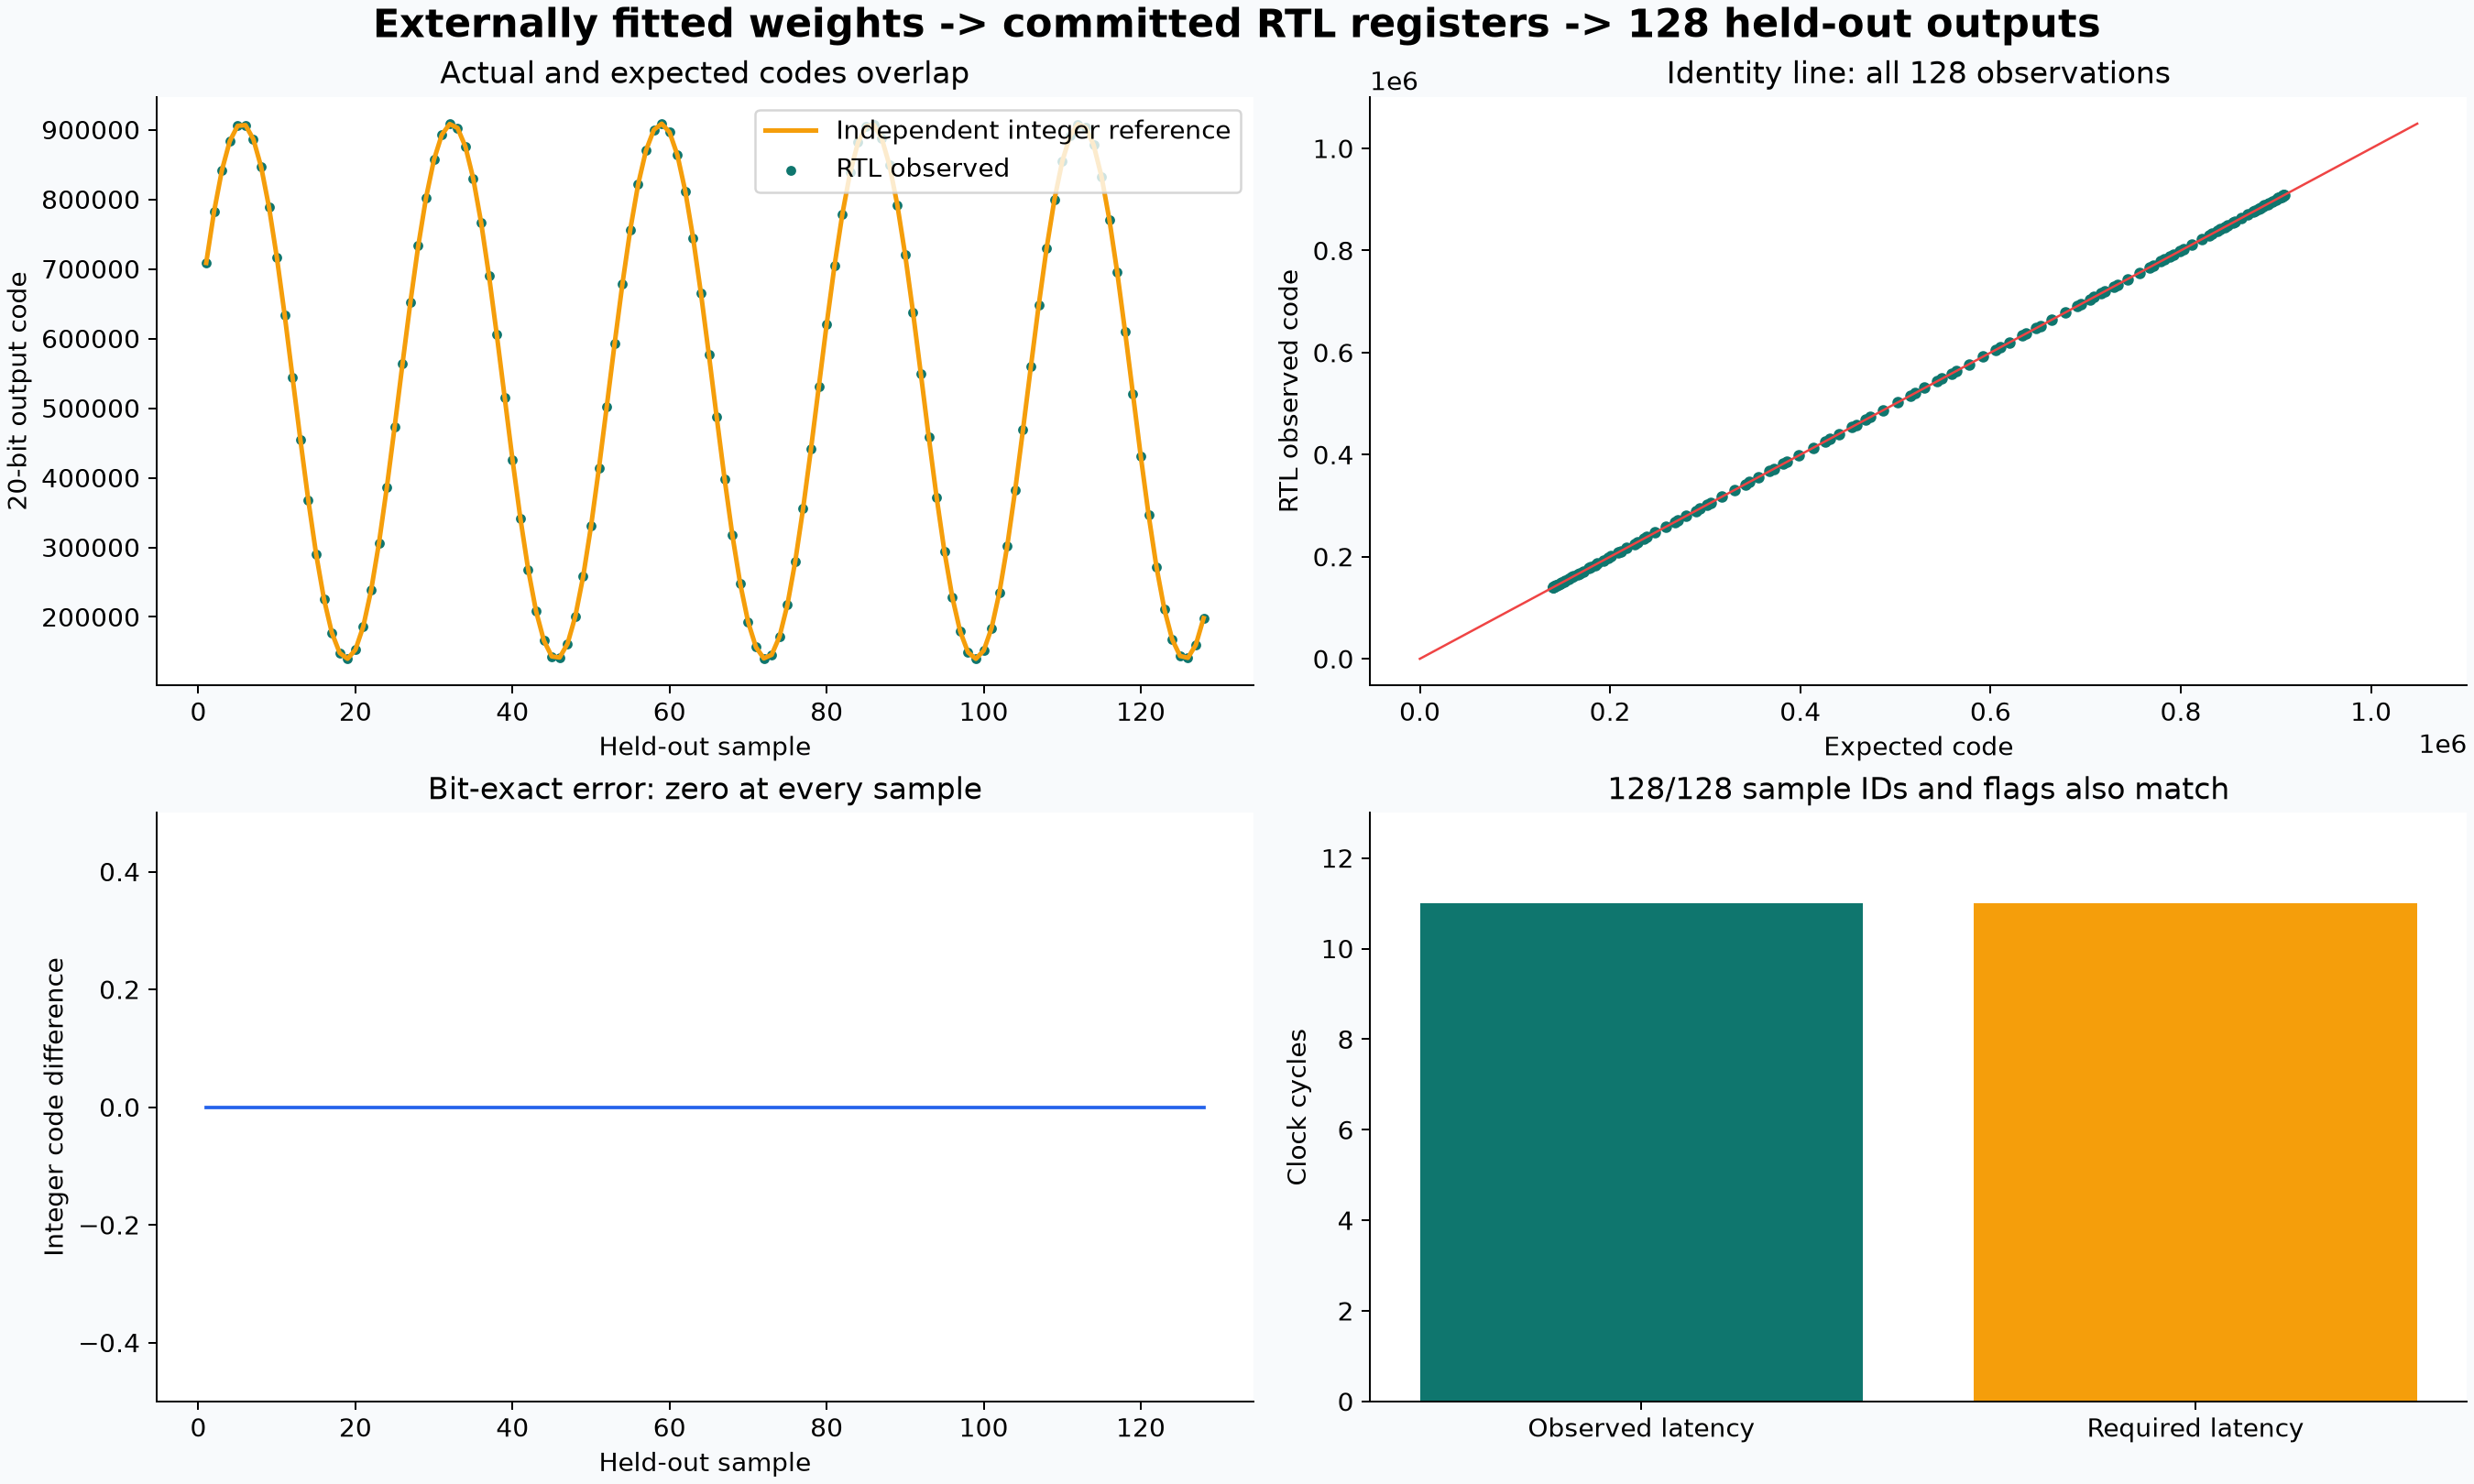
\includegraphics[width=.94\textwidth]{figures/17_fitted_holdout.png}\caption{外部拟合权重加载后 128 笔留出样本的实际 RTL/期望码、flags、ID、11 拍延迟；来自 CI 原始日志。}\end{figure}
\begin{figure}[H]\centering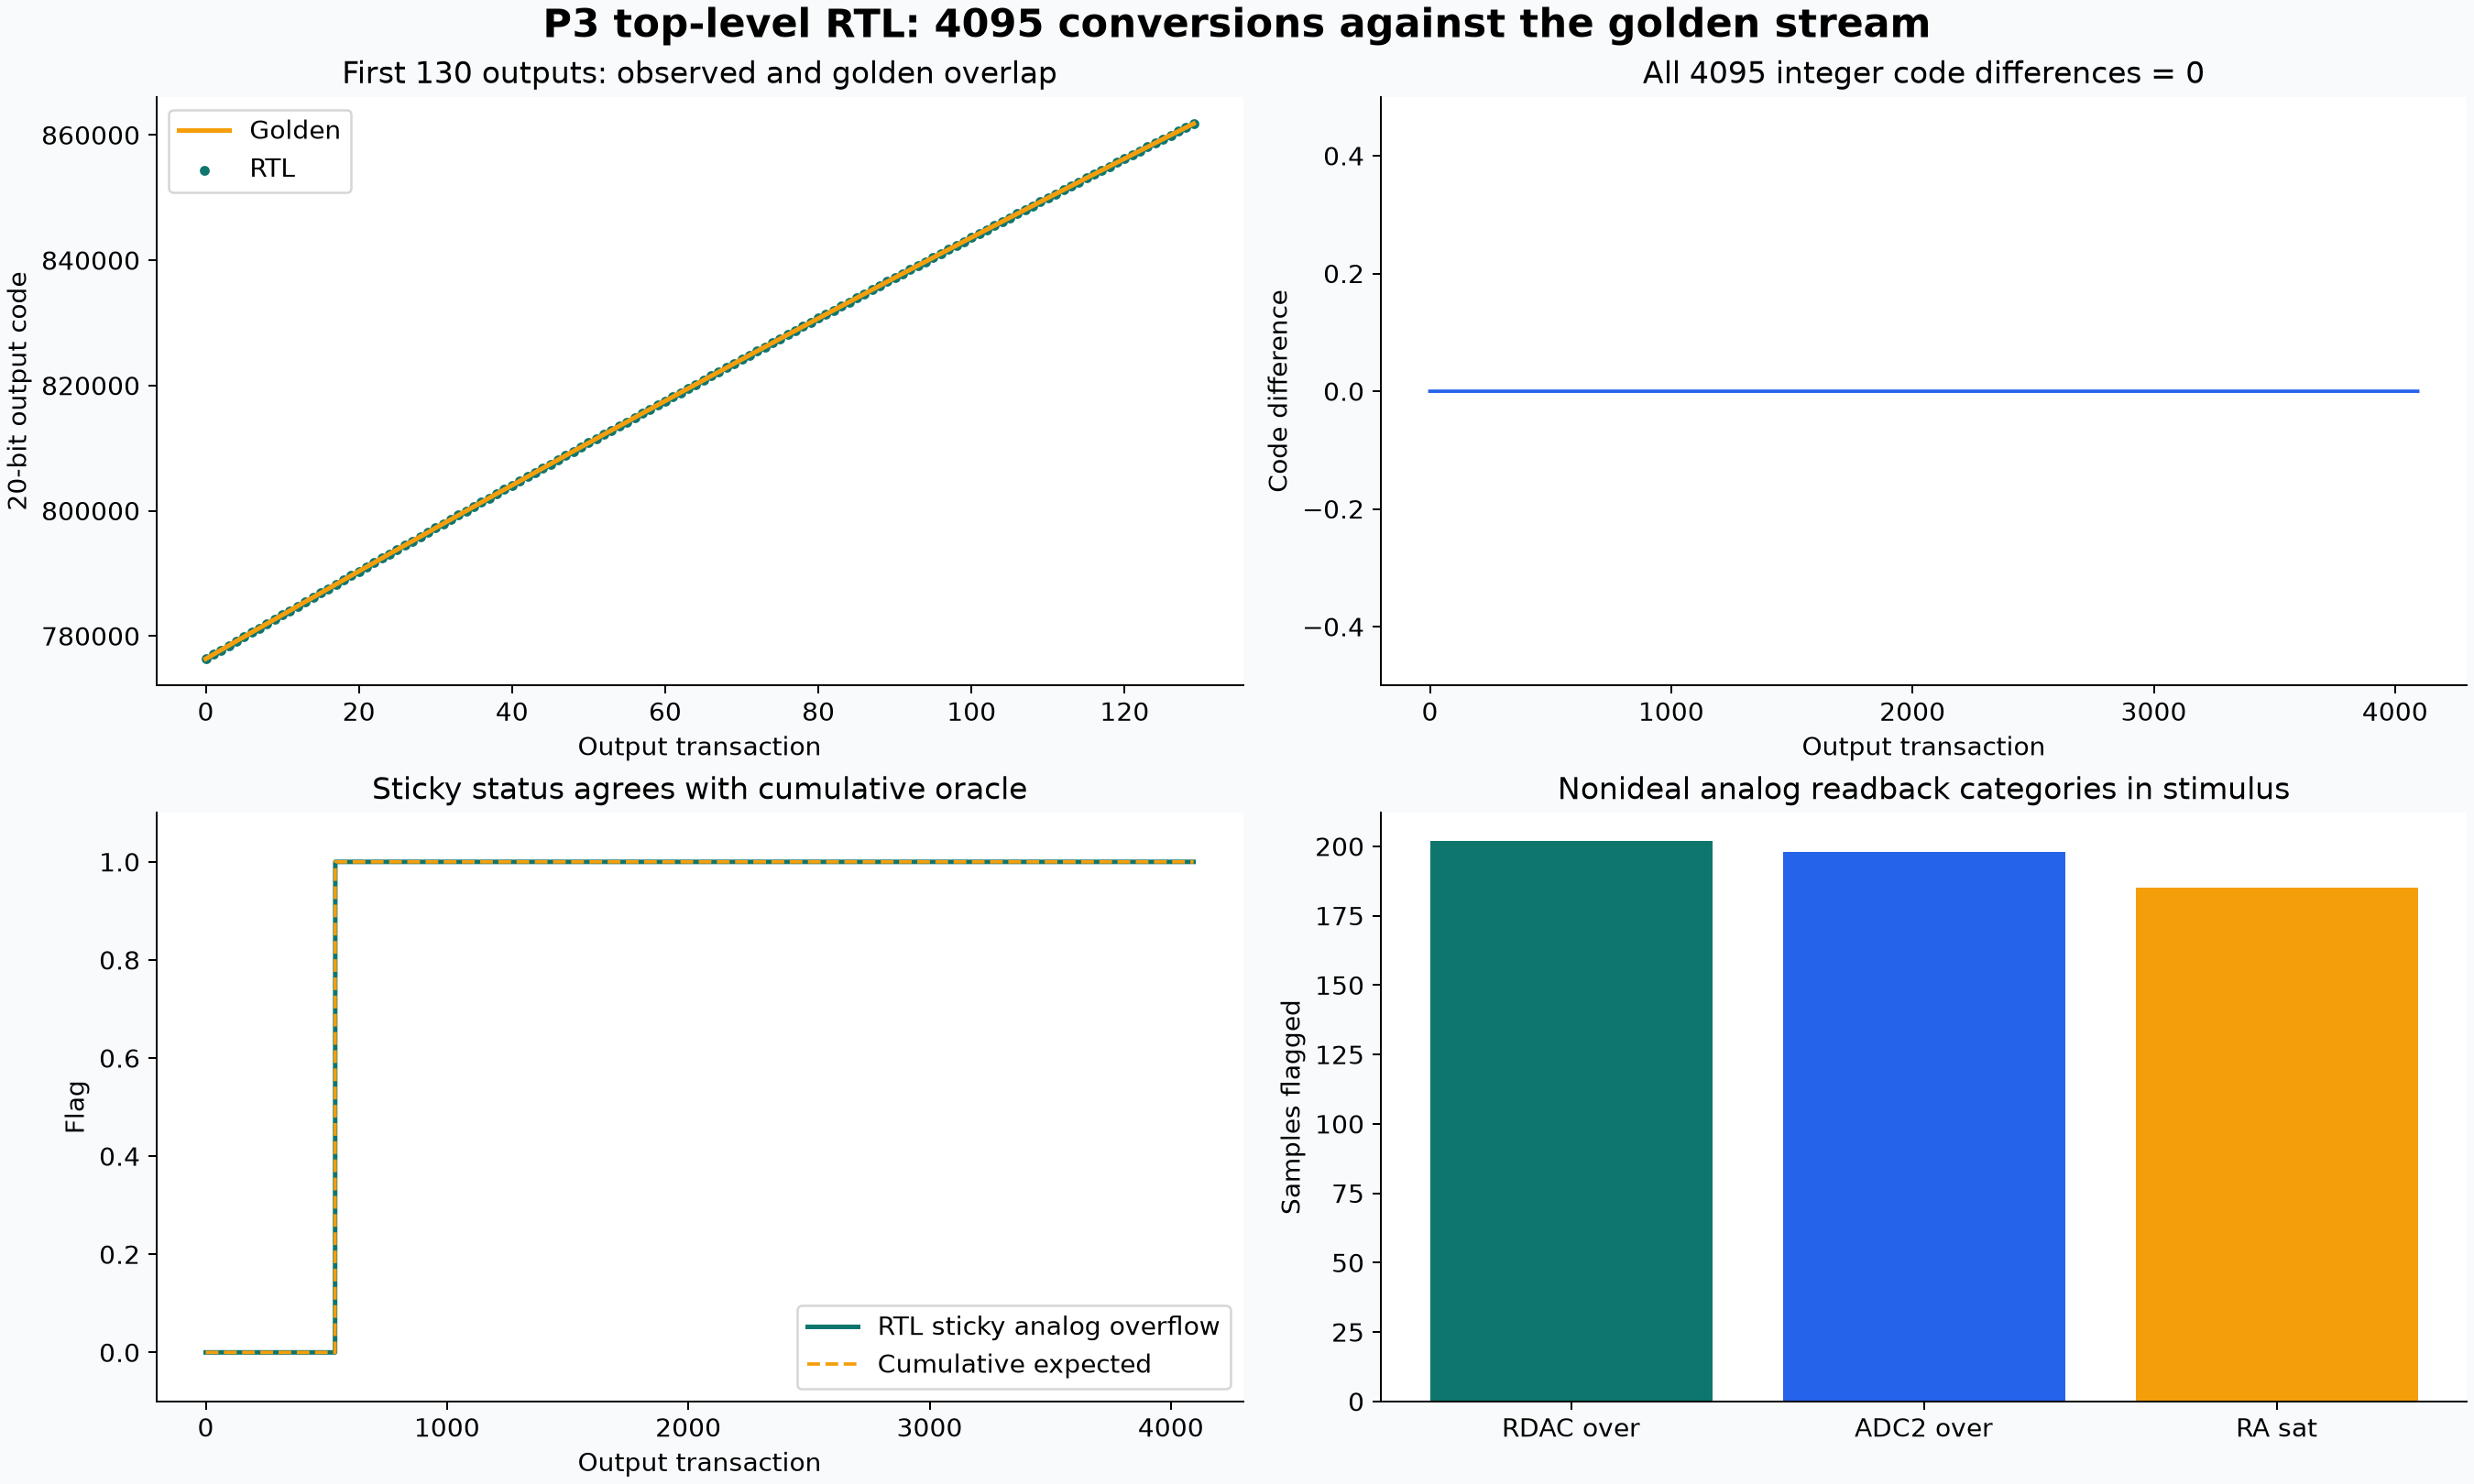
\includegraphics[width=.94\textwidth]{figures/18_p3_waveforms.png}\caption{兼容模式顶层 4095 笔实际码、期望码与标志。dither 源由 testbench force 替代；模拟回读是行为激励，ID 端口未连接。}\end{figure}
\begin{figure}[H]\centering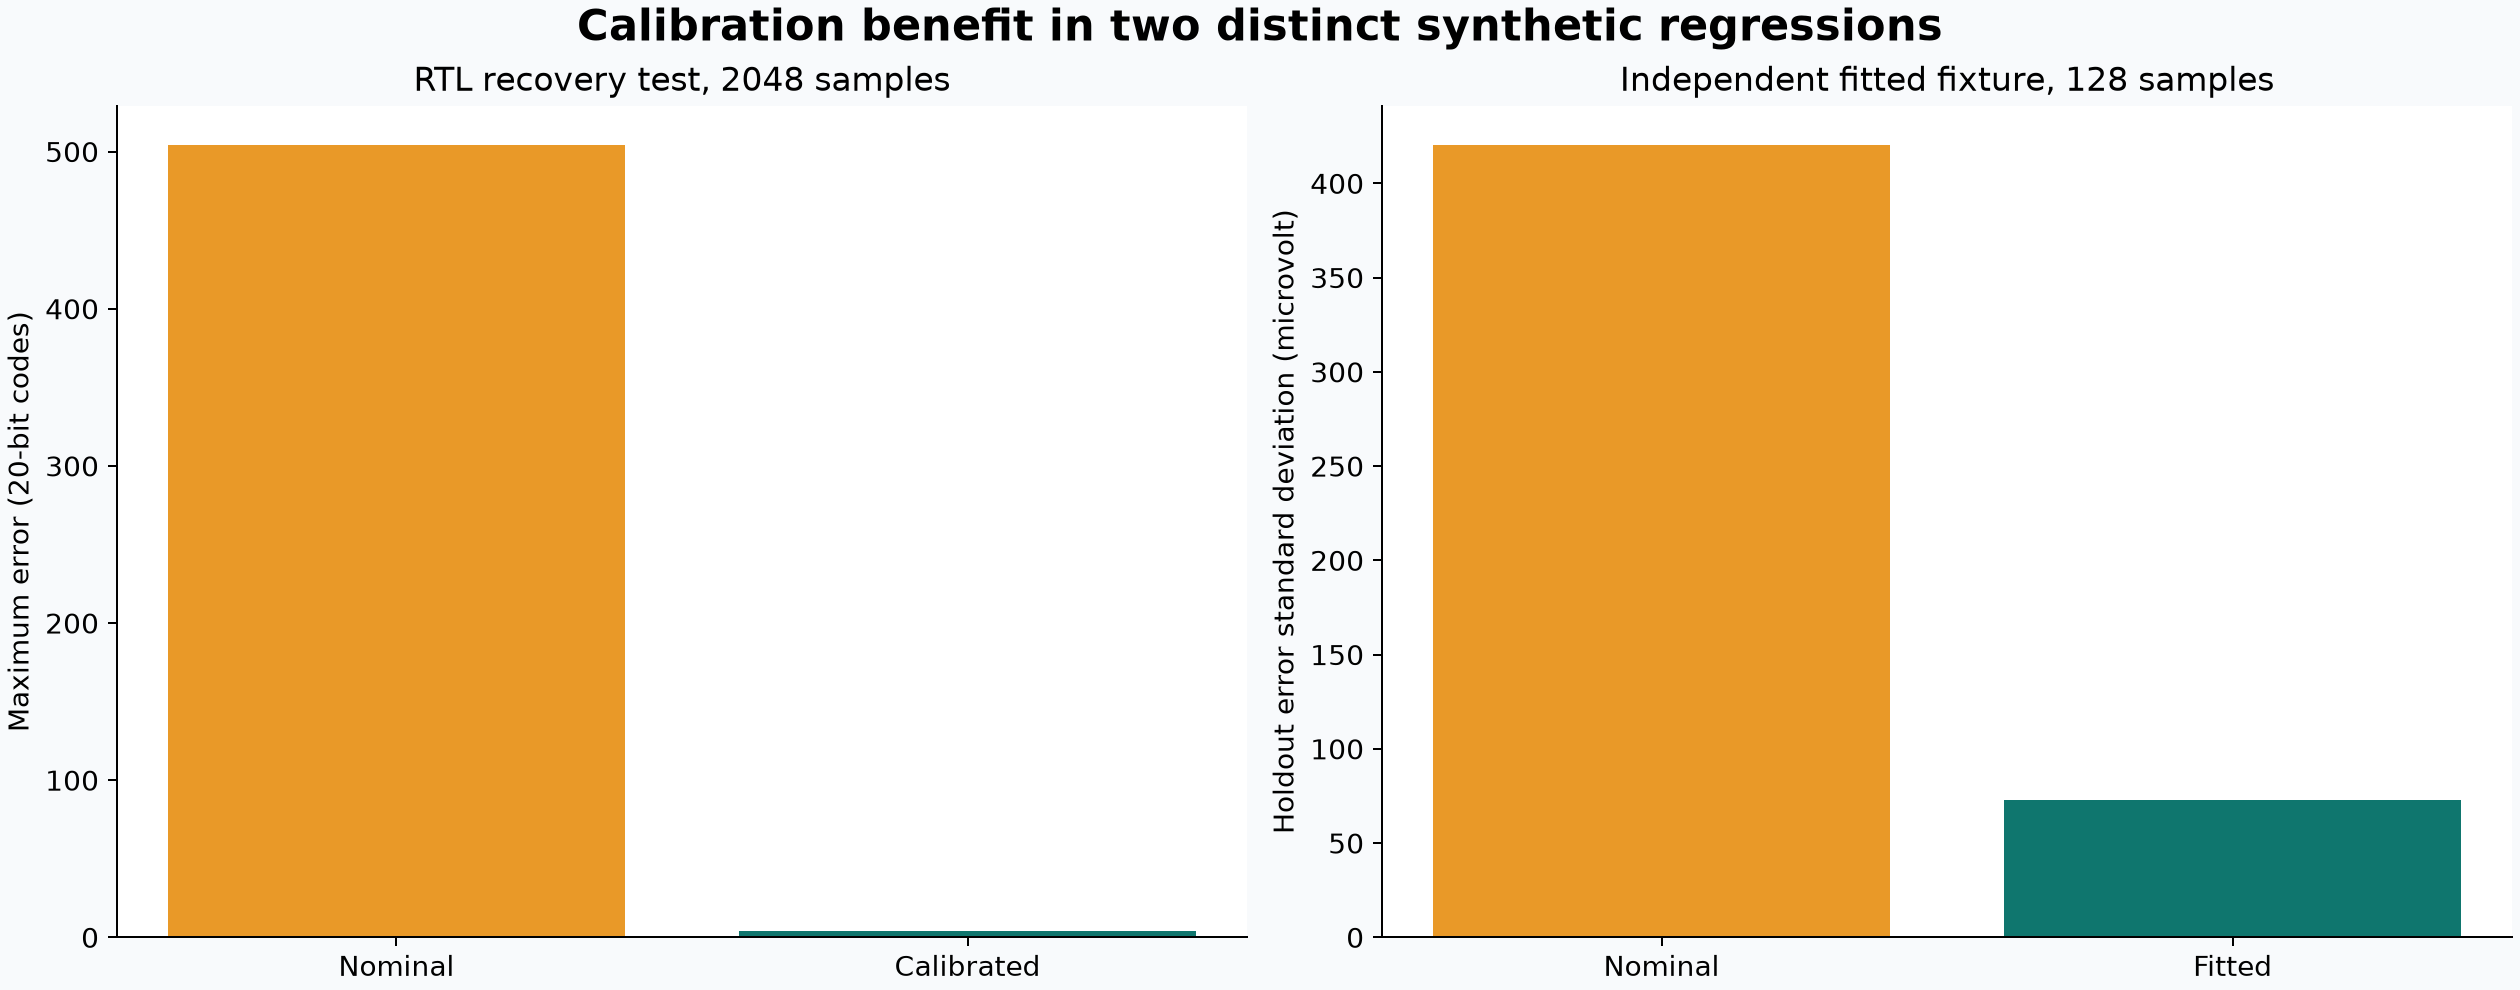
\includegraphics[width=.9\textwidth]{figures/21_calibration_benefit.png}\caption{合成失配的两种校正指标；数值口径不同，不可直接换算为芯片 ENOB。}\end{figure}
\begin{figure}[H]\centering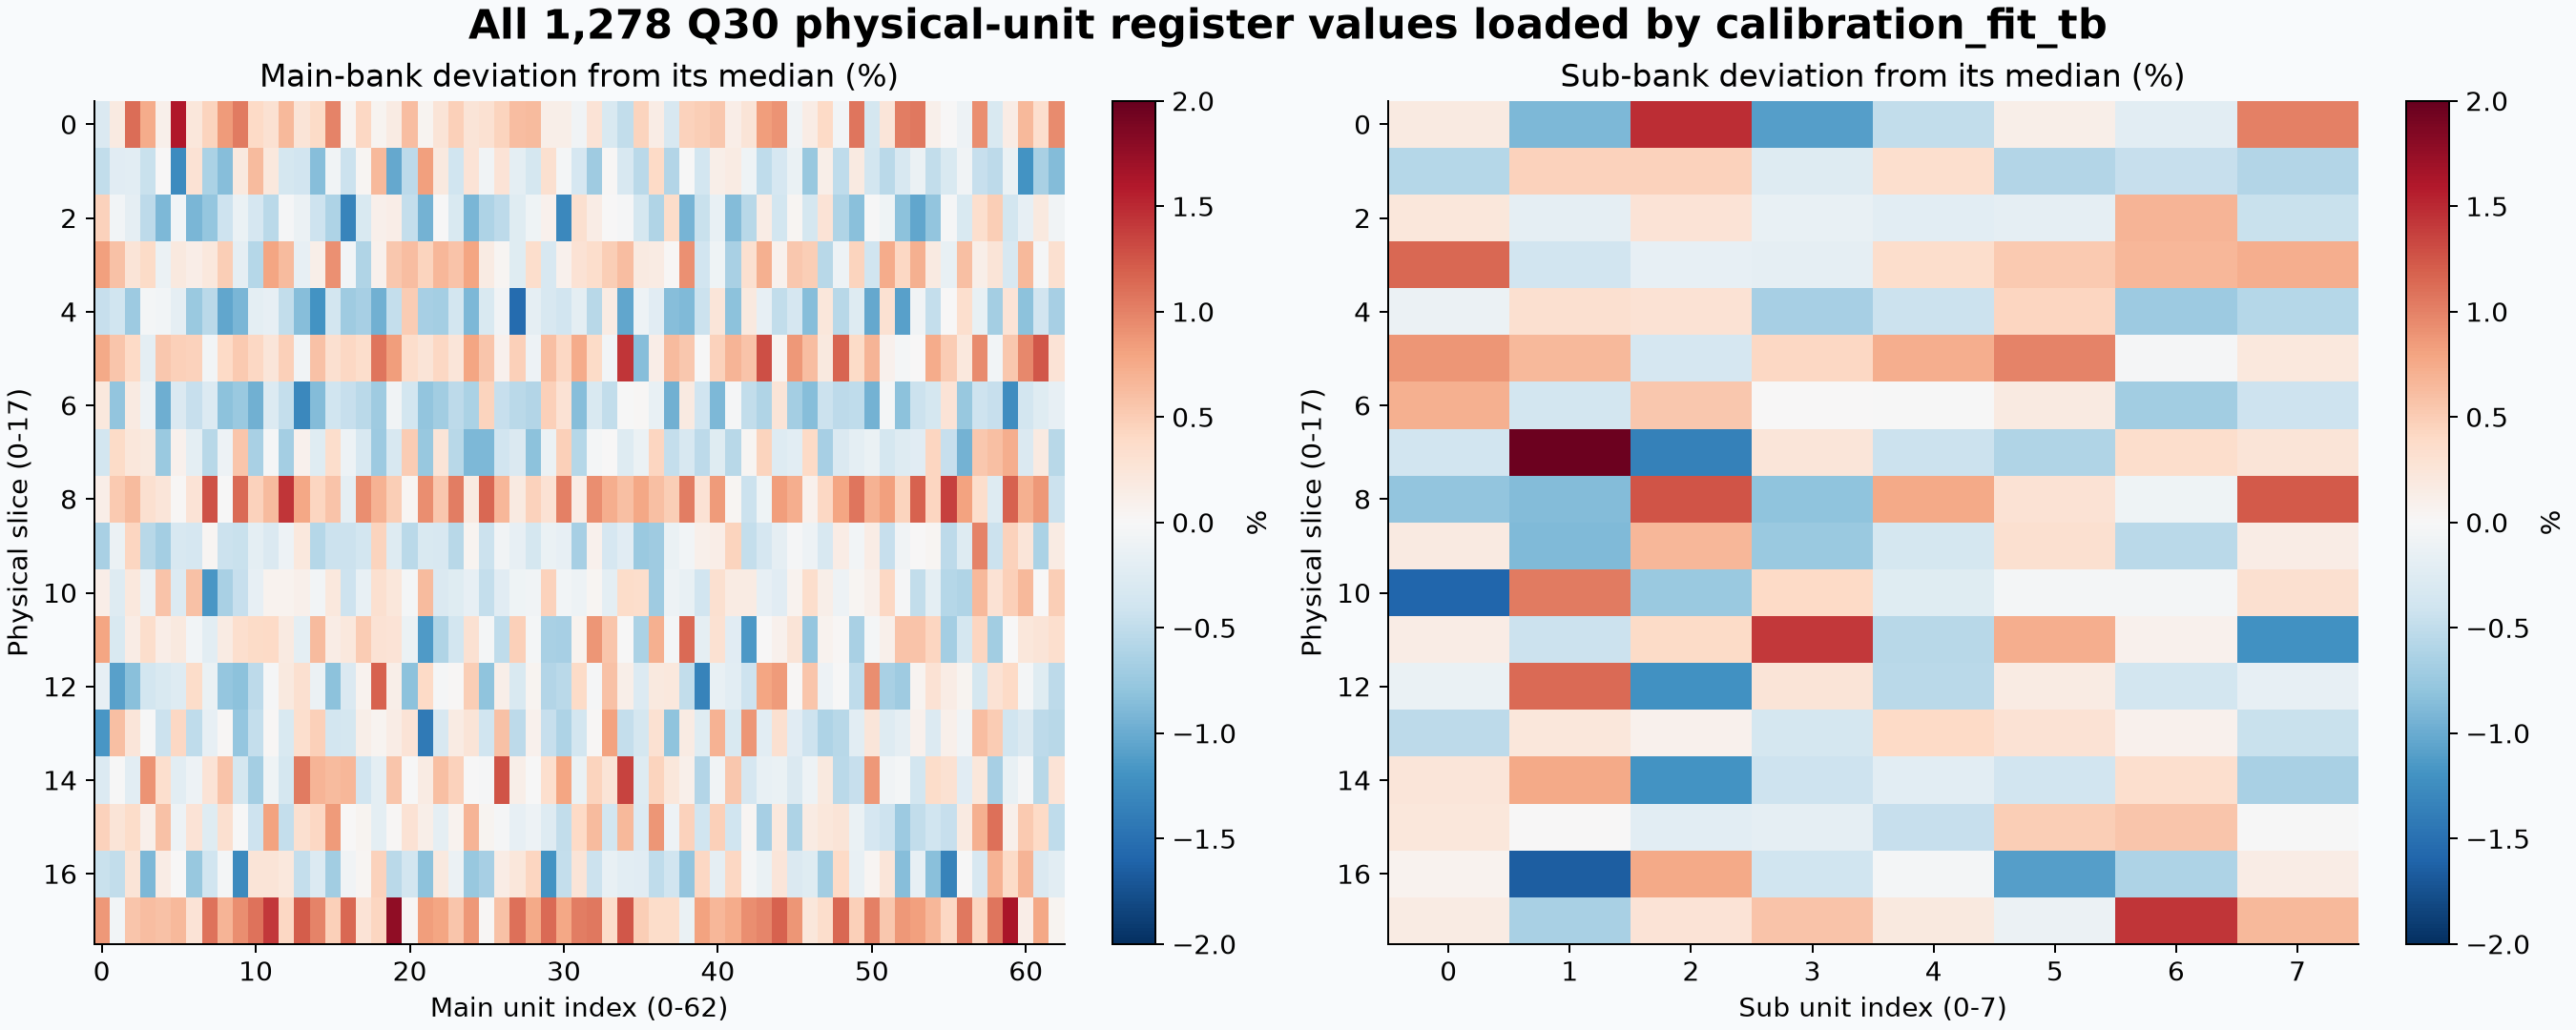
\includegraphics[width=.9\textwidth]{figures/22_fitted_weight_map.png}\caption{18$\times$71 物理权重装载镜像；证明地址内容，不证明电容真值。}\end{figure}

\section{每个“成功”的精确定义}
SAR bench 证明给定同步比较器答案和有效握手下码序列正确，未测量动态比较器在1.5625\,ns内的复位与判决。全码 oracle 在 1 slice、2 个主单元和 1 个子单元、20-bit ADC2 的固定构造参数下检查 dout 等于输入码及 11 拍延迟，未覆盖生产尺寸 18×71 的所有权重和开关状态，也未覆盖未知模拟误差。校准留出 128 笔证明拟合镜像确实送入 RTL 后与独立期望码一致；它不证明真实芯片的未知权重可由相同激励唯一辨识。P3 输出图证明 4095 笔兼容数字链路的 16 拍间隔与码匹配；其 DUT ID/flags 端口未连接，图中横轴是测试台计数，不能作为 ID 证据；它不能证明论文的 40\,MS/s 和噪声指标。DEM/dither 直方图证明伪随机序列统计及开关译码的模型属性；失配噪声整形和频谱 spur 必须在带版图相关失配的混合信号模型或硅片上测量。


\section{最新22个测试台的完整覆盖索引}
下表逐项核对前代缓存版本\code{ci_rtl_417f/}的原始日志及完成标记，每行均已通过。22项包含原16个测试台，以及结构协议、参数延迟、除法穷举、树映射RTL见证、扩展归约miter和新增行和缓存测试。归约miter另有独立逐单元算术参考，能检测多个实现共同错误。这里的\code{tree_mapping_tb}只表示RTL运行，真实XSim网表运行在第\ref{ch:synthesis-repair}章另列。每项通过均受其激励限制，测试次数不等于独立场景数；本次同job的独立算术审计已通过，旧轮入口失败按历史来源单列。
\small
\begin{longtable}{>{\raggedright\arraybackslash}p{46mm}>{\raggedright\arraybackslash}p{108mm}}
\toprule 测试台&成功判据与明确边界\\\midrule\endfirsthead
\toprule 测试台&成功判据与明确边界\\\midrule\endhead
\code{sar_trial_tb}&12-bit 4096 码与9-bit 512码；检查握手停顿、最终码和cancel；比较器是理想同步模型。\\
\code{calibration_recovery_tb}&2048 个缩小阵列合成失配样本，校准最大误差4码、名义权重504码；误差预算含ADC2量化，非INL硅测。\\
\code{calibration_fit_tb}&1278项真实寄存器加载/读核对；128条实际FIT\_ROW含码、flags、ID和11拍延迟，全部匹配。\\
\code{structural_adc_tb}&三种配置、438输出、7680次检查，覆盖18物理slice与缺失判决后的恢复；端口驱动理想比较器。\\
\code{structural_protocol_tb}&120帧、57笔提交、63笔预期丢弃、1920次检查、2次译码扰动；检查截止、恢复、ID和注入归属。\\
\code{recon_ppa_latency_tb}&P5/P6/P7各32笔连续事务；II=16，busy释放14/12/10拍，输出延迟15/13/11拍。\\
\code{divider_borrow_tb}&六种位宽/展开组合共67592个穷举输入；floor定义式、除零、固定延迟、busy拒绝、结果保持和done单拍。\\
\code{tree_mapping_tb}&12904次独立标量比较；Flash、物理权重、模式、全地址编码和随机系数；本行仅指RTL见证。\\
\code{cal_weight_reduce_ppa_tb}&七种几何共1430848次原实现/列归约/缓存实现及独立标量比较；生产尺寸枚举43758种8-of-18集合并交叉轨与采样模式。\\
\code{weight_row_cache_tb}&五种几何共16150步骤；逐写核对物理行和、合法/非法写、重复地址替换、clear保值及最大权重。32$\times$128完整表与18$\times$71生产几何均覆盖。\\
\code{calibration_physical_tb}&2048事务，18个slice、每个7+1单元的缩小夹具；256-bit整数oracle检查掩码、注入、取整、剪裁、ID与无效ID。\\
\code{review_top_protocol_tb}&1108次检查、38输出；兼容profile固定相位捕获、缺失ready、恢复与非强制dither路径。\\
\code{review_leaf_tb}&91142次检查，叶模块边界、参数守卫和组合译码；不等于门级毛刺或模拟建立验证。\\
\code{review_recon_protocol_tb}&未配置启动、配置撤销、完成/错误位与样本ID；观察有效结果和禁止泄漏的事务。\\
\code{review_dither_tb}&7组幅值/种子，每组200000次候选抽样；有效接受数、分布、均值、自相关和保持/复位检查。\\
\code{review_config_tb}&624个输出，完整性/运行锁定/写入冲突等配置回归；不表示外部总线CDC已验证。\\
\code{p2_tb}&23049次检查，除法、重构、剪裁、溢出、11拍延迟；百万码扫描由独立oracle承担。\\
\code{p2_oracle_tb}&1048576个码，固定小尺寸构造下dout等于输入及11拍延迟；非全部物理系数空间枚举。\\
\code{p2_periph_tb}&709次检查，配置外设与状态/存储不变量；0 error。\\
\code{p2_smoke_tb}&1154次检查，各分项零失配；链路冒烟而非全部结构覆盖。\\
\code{p1_tb}&464823次检查，DEM状态/地址、交换、温度计和链路；七个分项零错误。\\
\code{p3_top_tb}&4095笔兼容profile输出、16386检查、0 error；force替代dither源，DUT ID/flags未接，不构成其证据。\\
\bottomrule\end{longtable}
\normalsize
\section{本轮新增的独立算术与结构证据}
任意精度Python oracle独立生成90,058个向量：残差MAC 40,010个、ADC2解码40,000个、63/64-bit除法10,048个；另有8组输出标志序列。覆盖合法最小负值、96-bit边界、floor负商、半值向偶、非法范围与busy期间重复start。参考生成器没有导入被测RTL镜像；故意破坏最小负数判定与除法位组顺序，两项负控均被测试抓到。所有通过结论受其向量范围限制。

结构协议新增120帧：57笔应提交、63笔应丢弃；共1,920次检查，逐个粗/细SAR决策位置丢失valid，检查截止、迟到活动、恢复、ID与注入归属。在时钟沿之间施加两次相位总线扰动，旧版和取消信号变异版分别在234/242\,ns失败，修复版通过。该测试证明数字使能不再直接响应所施加的译码扰动；不是门级延迟模型或物理无毛刺保证。

\begin{figure}[H]\centering
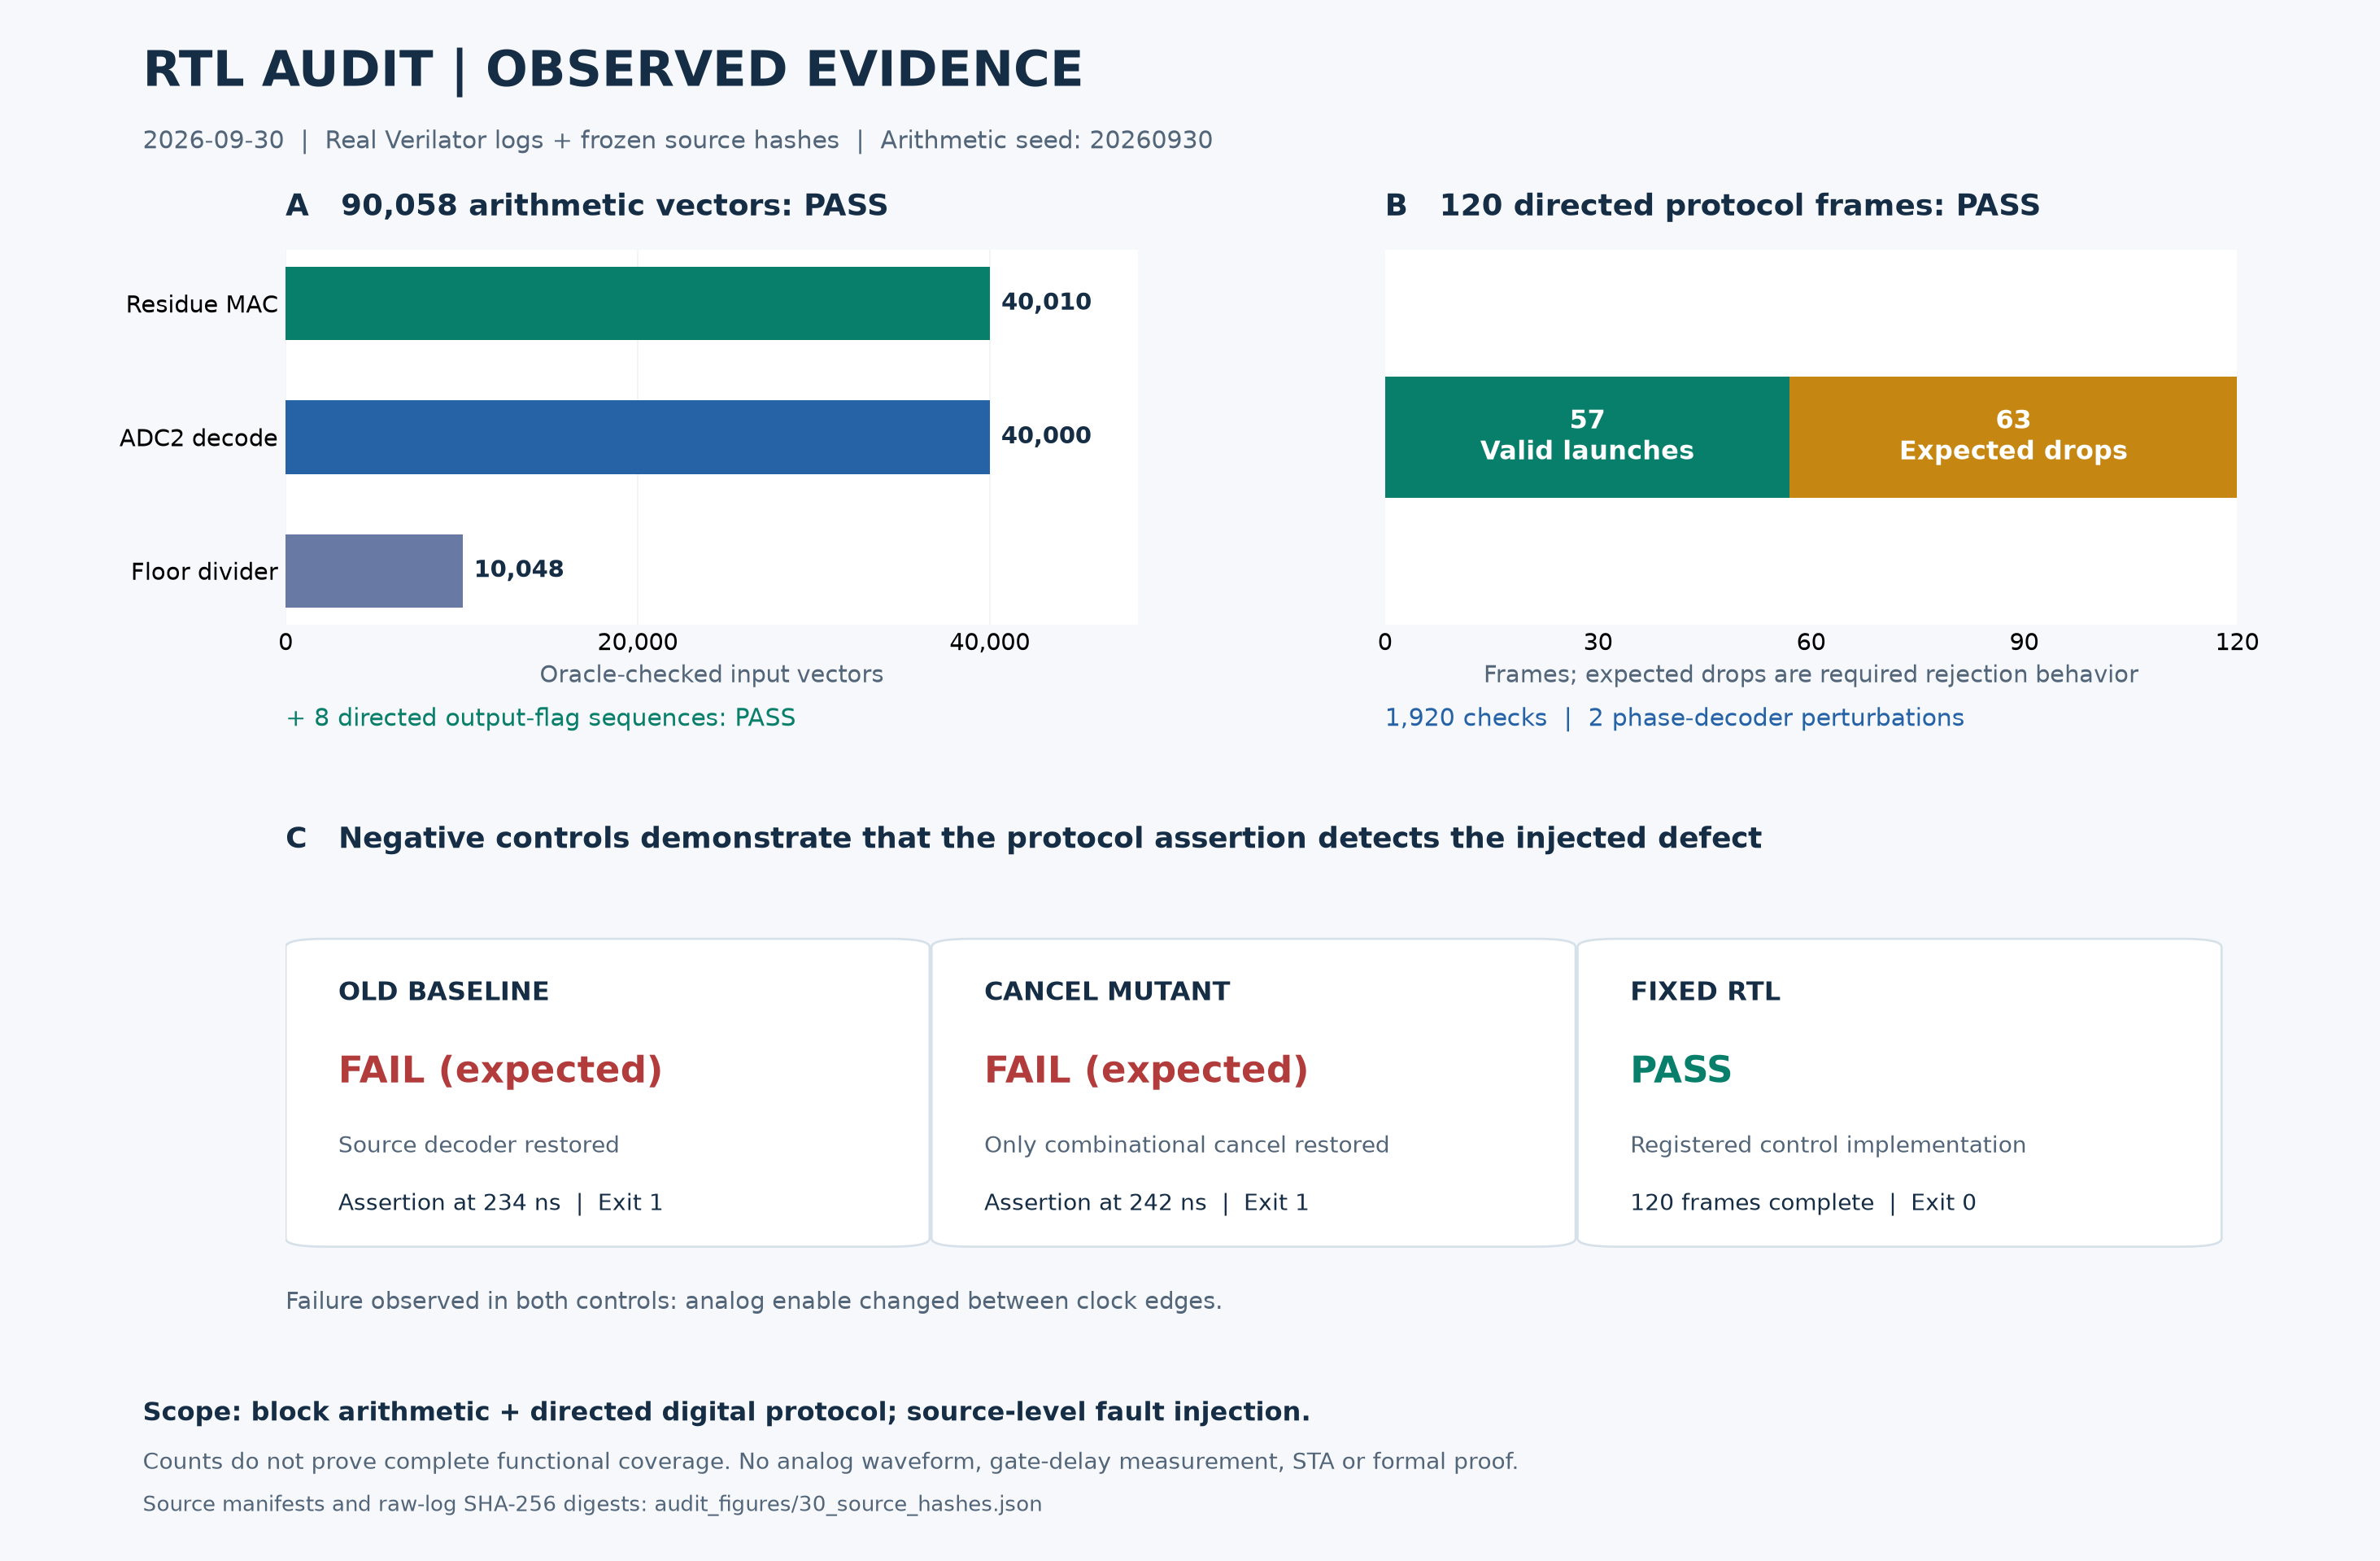
\includegraphics[width=\textwidth]{figures/30_arithmetic_protocol_audit.png}
\caption{首轮定向实跑日志与manifest的证据概览；后续跨版本审计另立来源。每个计数都有原始数据；图是覆盖样本和判据的展示，不是人为绘制的电路波形。}
\end{figure}

面积导向归约另有新旧模块并排miter：7种几何、1,430,848次逐位比较，全部通过。生产几何枚举所有43,758种8-of-18集合，交叉16种轨模式和2种采样模式；同时测试极值、重复/越界ID和合法随机重排。落地版本再通过物理校准2,048样本、恢复2,048样本、拟合权重128样本/1,278系数，以及1,048,576码小尺寸全码oracle。miter有配套整数代数与位宽论证，但仍不应称为全设计形式等价证明。

\chapter{仿真证据的可信度、对照实验与复现方法}
\label{ch:evidence-method}
本章把“仿真成功”拆解为可以独立检查的工程命题。前面的证据图展示现有结果；这里解释为什么选择这些测试、每张图能排除什么错误，以及哪些结论还不能从它推出。所有数字仿真图与模拟电路波形分开标注，生成图形本身不构成通过判定。

\section{从需求到判据的四层关系}
第一层是目标，例如支持一个配置 epoch 下的 16 拍采样间隔。第二层是实现契约，例如采样捕获在哪一个沿发生、转换截止时如何取消、后级结果使用哪个 ID。第三层是激励，例如在第 \(k\) 次 SAR 判决时撤销 valid。第四层是独立判据，例如本帧不提交、下一帧恢复、恢复结果的物理选择和 ID 均正确。省掉中间两层，很容易得到只会打印 PASS 的测试台。

一个完整记录至少包含：源文件 SHA、参数镜像、工具版本、命令行、随机种子或向量文件 SHA、编译退出状态、运行退出状态、完成标记和错误计数。若命令缺失、编译超时或日志来自旧文件，即使目录里还有上一轮 PASS，也必须失败。现有独立算术 runner 对缺工具和陈旧日志有负控；Vivado runner 则进一步要求工件完整、status 与报告条件一致，并拒绝已发现的无驱动综合告警。

\begin{table}[htbp]\centering\small
\begin{tabularx}{\textwidth}{p{25mm}X X}\toprule
层级&有用问题&不能替代的下一层\\\midrule
行为模型&架构关系、误差项与算法是否自洽？&不证明 RTL 的位宽、握手和综合语义。\\
RTL 仿真&整数码、异常与样本协议是否匹配？&不证明工具映射后逻辑仍完整。\\
综合网表功能&关键输入确实影响输出，映射函数正确？&不证明布局布线后达到时钟和功耗目标。\\
实现后 STA/仿真&指定 FPGA、约束和时序角是否收敛？&不证明目标 ASIC 工艺及模拟电路指标。\\
混合信号/PVT&模拟建立、比较器、参考与数字共同工作？&不等于制造后硅片测量。\\
\bottomrule\end{tabularx}
\caption{证据层级及不可越过的推论边界。}
\end{table}

\section{正确值测试与负控测试的区别}
正常值测试回答“已知场景下输出是否正确”。负控测试有意引入一个确定错误，回答“当前测试是否真的能区分这个错误”。如果把最小负值的合法下界写错后，原测试仍全部通过，就不能称它覆盖了有符号边界。

本轮算术负控改变合法最小负值判定和除法位组顺序；结构协议负控恢复旧的组合相位译码或单独恢复旧取消信号。故障均在独立变异副本中注入，生产 RTL 不被污染。应保存变异补丁、命令、预期失败位置和实际失败日志。只记录“负控失败”不足以说明它因目标故障失败，也可能是编译语法损坏；因此需要定位到可解释的断言或逐笔失配。

综合完整性需要类似的负控。基线实际暴露的 \code{Synth 8-3848} 不是人为选择的测试错误，而是真实工具风险；门禁测试应在模拟日志中插入同一告警格式，确认即使工具 raw return code 为 0、status 文件齐全，最终评审状态仍被拒绝。正常无关 warning 则不能被一概当成失败，以免用户学会忽略整套门禁。

\subsection{为什么使用两个独立参考层}
对完整系统，参考模型需要重用物理参数定义才能保持接口一致；但若 oracle 与被测实现复制了同一段位操作，错误也会一起复制。独立任意精度 oracle 从数学定义计算，不导入 RTL 镜像表达式，用来检验乘加、解码和 floor。系统测试再用真实地址/配置/时序驱动完整链路，用来检验集成。

两者互相补足：独立算术不能发现系数写错物理地址，系统斜坡也可能看不到最小负数边界。所谓独立并不是完全没有共享任何常量；正确做法是公开哪些输入定义共享、哪些运算实现独立，以及生成器是否调用了被测公式。

\section{各类图怎样读取才不误判}
\subsection{码值与差值}
上层图可画实际码和期望码，便于观察范围、单调性和样本缺失；下层必须画差值或逐笔错误标记，因为百万级码范围会把一个 LSB 的失配掩盖。通过判据来自全部原始样本的整数比较，图中抽样用于显示，不能反过来用稀疏像素证明全数据一致。

横轴应注明是 DUT sample ID、测试台序号还是时间。兼容顶层 P3 的图来自测试台计数，其 DUT ID/flags 端口未接，不能作为跨样本 ID 正确的证据。结构协议与拟合留出测试则显式检查 ID。即使两张图横轴都写“sample”，其证明能力也不同。

\subsection{误差改善图}
校准恢复夹具的最大误差从名义权重的 504 码降为 4 码，说明对所注入的固定合成失配，载入系数和整数校正有明显效果。这不是 SNDR、ENOB 或 INL 的等价表述。要计算 ENOB，需要明确频率、幅度、采样率、长度、窗函数和噪声/失真处理；要计算静态 INL/DNL，则需要转移特性或规定的码密度实验。把误差改善比直接取对数写成动态范围会混淆量纲和测量定义。

\subsection{延迟和协议波形}
延迟以接受 start 的有效沿为零点，而不是以驱动器试图发 start 的时刻为零点。busy 期间的 start 被拒绝时，不应计入成功事务。完成边沿和下一次启动边沿可能不同；因而同时记录结果延迟、busy 释放时刻和可接受下一样本的间隔。

P5/P6/P7 的 15/13/11 拍重构延迟由两个范围不同的夹具核对。最新精简权重 RTL 已在 \code{ci_rtl_0c4a/} 的连续启动夹具中对每档重跑32笔、间隔16拍的请求，检查无合法样本丢失及 busy 在14/12/10拍释放。该夹具使用缩小阵列。\code{compact_profiles/} 另运行生产18-slice结构顶层：每档检查438次输出、438次精确延迟和7,680个协议节拍，三档仍分别得到15/13/11拍。两项均有当前内容摘要对应的实际日志；旧 \code{final_profiles/} 仅作历史归档保留。

这些是 RTL 协议和功能仿真的拍数，不能证明实际 FPGA 的每一拍都能做到约 1.563 ns。仿真中的时钟周期是激励条件，只有加入正确的延迟模型并满足实现时序后，才能把它与物理频率联系起来。

\section{覆盖矩阵的实质内容}
覆盖矩阵应围绕故障机制组织，不能只按文件名列出“已测”。例如，采样注入符号、主子组权重排列和负数 floor 都会影响最终码，但需要不同激励才能区分。下面给出本工程已有测试与应继续补足的关系。

\small
\begin{longtable}{>{\raggedright\arraybackslash}p{29mm}>{\raggedright\arraybackslash}p{47mm}>{\raggedright\arraybackslash}p{70mm}}
\toprule 故障机制&已有区分证据&仍需保留的边界\\\midrule\endfirsthead
\toprule 故障机制&已有区分证据&仍需保留的边界\\\midrule\endhead
正负号/隐式宽度&90,058 向量的独立整数对照与边界负控&有限测试不是对全部 64-bit 输入的形式证明。\\
物理地址错配&1278 项镜像加载、留出事务与物理校准夹具&真实电容版图地址和软件排序还需系统集成核验。\\
错误位晚一笔&定向异常、保持行为和当前 ID 检查&ADC2 告警与硬错误的消费策略需软件遵守。\\
跨相位污染&120 帧丢失 valid/迟到活动/恢复测试&异步模拟比较器的 CDC 和亚稳态不在零延迟 TB 内。\\
归约代数改写&两个 Verilator 版本各 1,430,848 次检查、7 个几何；新旧实现均对照独立 scalar oracle&补强后的判据检出共同错误；RTL 结果仍不能发现特定综合器丢失树。\\
前向引用综合差异&旧网表 warning、常量化及无扇出；两种连接修复见证均通过12904次XSim比较&小单元的输入因果与功能检查不能代替完整顶层的约束和实现验收。\\
除法组合链过深&真实 timing path 的 carry 级与起止寄存器&单独优化除法后，最坏路径可能转移到归约或 MAC。\\
配置并发冲突&完整性 bitmap、clear/validate/写入冲突回归&外部总线跨域协议不是当前同步接口自动提供。\\
\bottomrule\end{longtable}
\normalsize

\section{从波形追查一次失败的标准流程}
出现某笔最终码失配时，先确认其 sample ID 与配置 epoch，再确认 \(F,O,I\) 和 \(T,G,R\) 是否属于同一份快照。如果在这一步就发现物理选择不同，应优先定位上下文捕获和前后级调度，而不是调校算术公式。若输入快照完全一致，再把每一级整数中间值导出给任意精度 oracle，查出第一个不一致的操作。

对边界失败，保留数值的十六进制位型和有符号十进制解释。只看十进制有时会忽略截断位宽，只看十六进制又不容易辨认负数。对时间失败，保留接受沿、deadline、cancel、valid、done 和输出沿；不要只截取最终报错时刻，因为根因可能发生在一个 frame 之前。

综合后失败还需多一层：检查优化日志和输入扇出，确认该输入仍参与目标函数。若某个功能块被综合成常量，先解决 elaboration 或约束问题，再看关键路径。对无驱动节点加 \code{keep} 不会创造本来缺失的驱动；增加 timing exception 更不能恢复逻辑。

\begin{figure}[htbp]\centering
\begin{tikzpicture}[>=Stealth,font=\small,node distance=7mm,b/.style={draw,rounded corners,align=center,text width=120mm,minimum height=10mm}]
\node[b] (i) {失配样本：固定源码 SHA、配置、向量与工具版本};
\node[b,below=of i] (c) {先检查 ID、epoch 和物理开关快照是否属于同一残差};
\node[b,below=of c] (a) {快照一致后，逐级核对 \(T,G,R,F,N,A,q\) 与独立整数 oracle};
\node[b,below=of a] (s) {只在综合网表失败时，检查 elaboration、驱动、扇出和常量传播};
\node[b,below=of s] (t) {功能成立后，再比较 setup/hold、关键路径、布局和功耗};
\draw[->](i)--(c);\draw[->](c)--(a);\draw[->](a)--(s);\draw[->](s)--(t);
\end{tikzpicture}
\caption{按因果顺序定位失配，避免把错误输出归因于尚未测量的模拟噪声。}
\end{figure}

\section{本轮 CI 编译超时与测试失败如何区分}
发布提交 \code{50b5733} 后，RTL CI 在七几何归约 miter 的 Verilator/C++ 编译阶段超过 300 s，尚未进入该 bench 的运行断言。该状态不是功能通过，也不是已经证实算术失败；正确记录是“此运行没有获得结果”。本轮将该大型 bench 的编译限时单独设为 900 s，并把 RTL job 总限时调整为 45 分钟，运行期仍使用单独的有限预算。

这项修复没有减少向量数、屏蔽断言或把超时改成成功。编译日志和运行日志分开保存，先删除旧的 run log，再创建新工件。对于其他普通 bench 仍保留原来的 300 s 编译限时，以便真实卡死及时暴露。旧版修复基线（RTL 内容摘要前缀 \code{169f957dc7fe}）曾在本地完整重跑 21 项 RTL 测试和 3 类 lint，\code{final_rtl/result.json} 记录该轮整体退出码 0 及 21 项完成标记；其中旧版归约 miter 记录全部 1,430,848 次比较。它使用当时的测试台和判据，不包含下节随后加入的独立 scalar 检查，也不能改标为精简权重存储版本的全量重跑。新提交的GitHub CI状态仍须独立确认，不能把本地通过或旧提交的绿色状态贴到新源文件上。

本轮本地全量回归还有一次构建环境失败：make调用的进程PATH里没有Python。该尝试没有有效仿真结果，原失败记录保留；补齐当次进程 PATH 后从旧版冻结源码完整重跑，才形成 \code{final_rtl/} 的历史成功证据。这个例子说明“环境修复”和“算法修复”应分别登记，避免把一次未运行的测试写成曾经算术失败。

\section{两份实现共同错误时，miter 为什么也会漏检}
提交 \code{39e9c27} 的后续 CI 在 Verilator 5.020 上进入实际运行后，
七几何归约 miter 于 \code{NS=32,NM=2,ND=1,DE=3} 的第 13 次检查失败。
这次不再是编译超时，不能沿用前一次故障解释。
用官方 5.020 源码构建的本机工具、原七实例 testbench、相同展开参数和优化级别，
再次观察到同一检查失败。

进一步保留原生成模型，只在相应 C++ 检查前增加诊断打印，发现更重要的现象：
前面的定向用例中，测试台权重已经为 1、8 个物理 slice 已选中，
但两份实现的 \(T\) 与 \(G\) 同时保持 0；独立数学值应为 24。
因此，miter 在首次报错之前已有双方共同偏离正确值的情况。
仅有 \(Y_{\rm new}=Y_{\rm old}\) 不能证明 \(Y_{\rm new}=Y_{\rm correct}\)。
当前工具生成代码把相关总和的赋值放在初始 settle 路径中，未随这类刺激按预期重算；
它是本次具体测试结构与工具组合的证据，不足以泛化为全部 packed-array 写入均有问题。

改进测试台时，保持生产 RTL、七种几何、随机种子、刺激顺序、43,758 种分配
以及全部原始比较不变，在明确的测试时钟沿捕获整包输入，
另一个沿以逐物理单元的 scalar oracle 同时检查新旧结果。
checker 与刺激生成分开，首个有效捕获沿安排在仿真启动之后；
每个几何还校验原有检查数量，避免忽略首样本或提前退出后仍打印完成。
这里只增加 testbench 的事务边界，没有给组合 DUT 增加生产流水级。
最终归档 \code{docs/evidence/20260930/reducer_scheduler/manifest.json} 记录：
修复后的同一测试台在 Verilator 5.020 与 5.49 下分别退出 0，
每次均出现七种几何的完成记录及总完成标记，检查总数各为 1,430,848。
生产尺寸的 43,758 个分配组合包含在上述计数中；两个工具运行同一激励集合，不能相加成更多覆盖。
对应 \code{after_5020.run.log} 与 \code{after_549.run.log} 保存原始结果，
被测归约器内容摘要前缀均为 \code{c5fc7f6ef58b}，也与 compact 版本一致。

共同错误负控只把两份实现共享的权重快照清零，保持原始刺激及 scalar oracle 不变。
5.020 运行在第 9 个检查点报参考值失配并以 134 退出：正确的 \(T,G,R\) 均为 24，
两份实现却均为 0。它说明新判据能识别原 miter 会接受的“双方同错”，
不把断言预期失败当作工具崩溃或成功仿真。
图\ref{fig:reducer-scheduler-evidence} 展示日志实际保留的前 16 个检查点及该负控，
原始失败日志与 printf-only 诊断副本一并保留，未覆盖历史运行。

\begin{figure}[htbp]
  \centering
  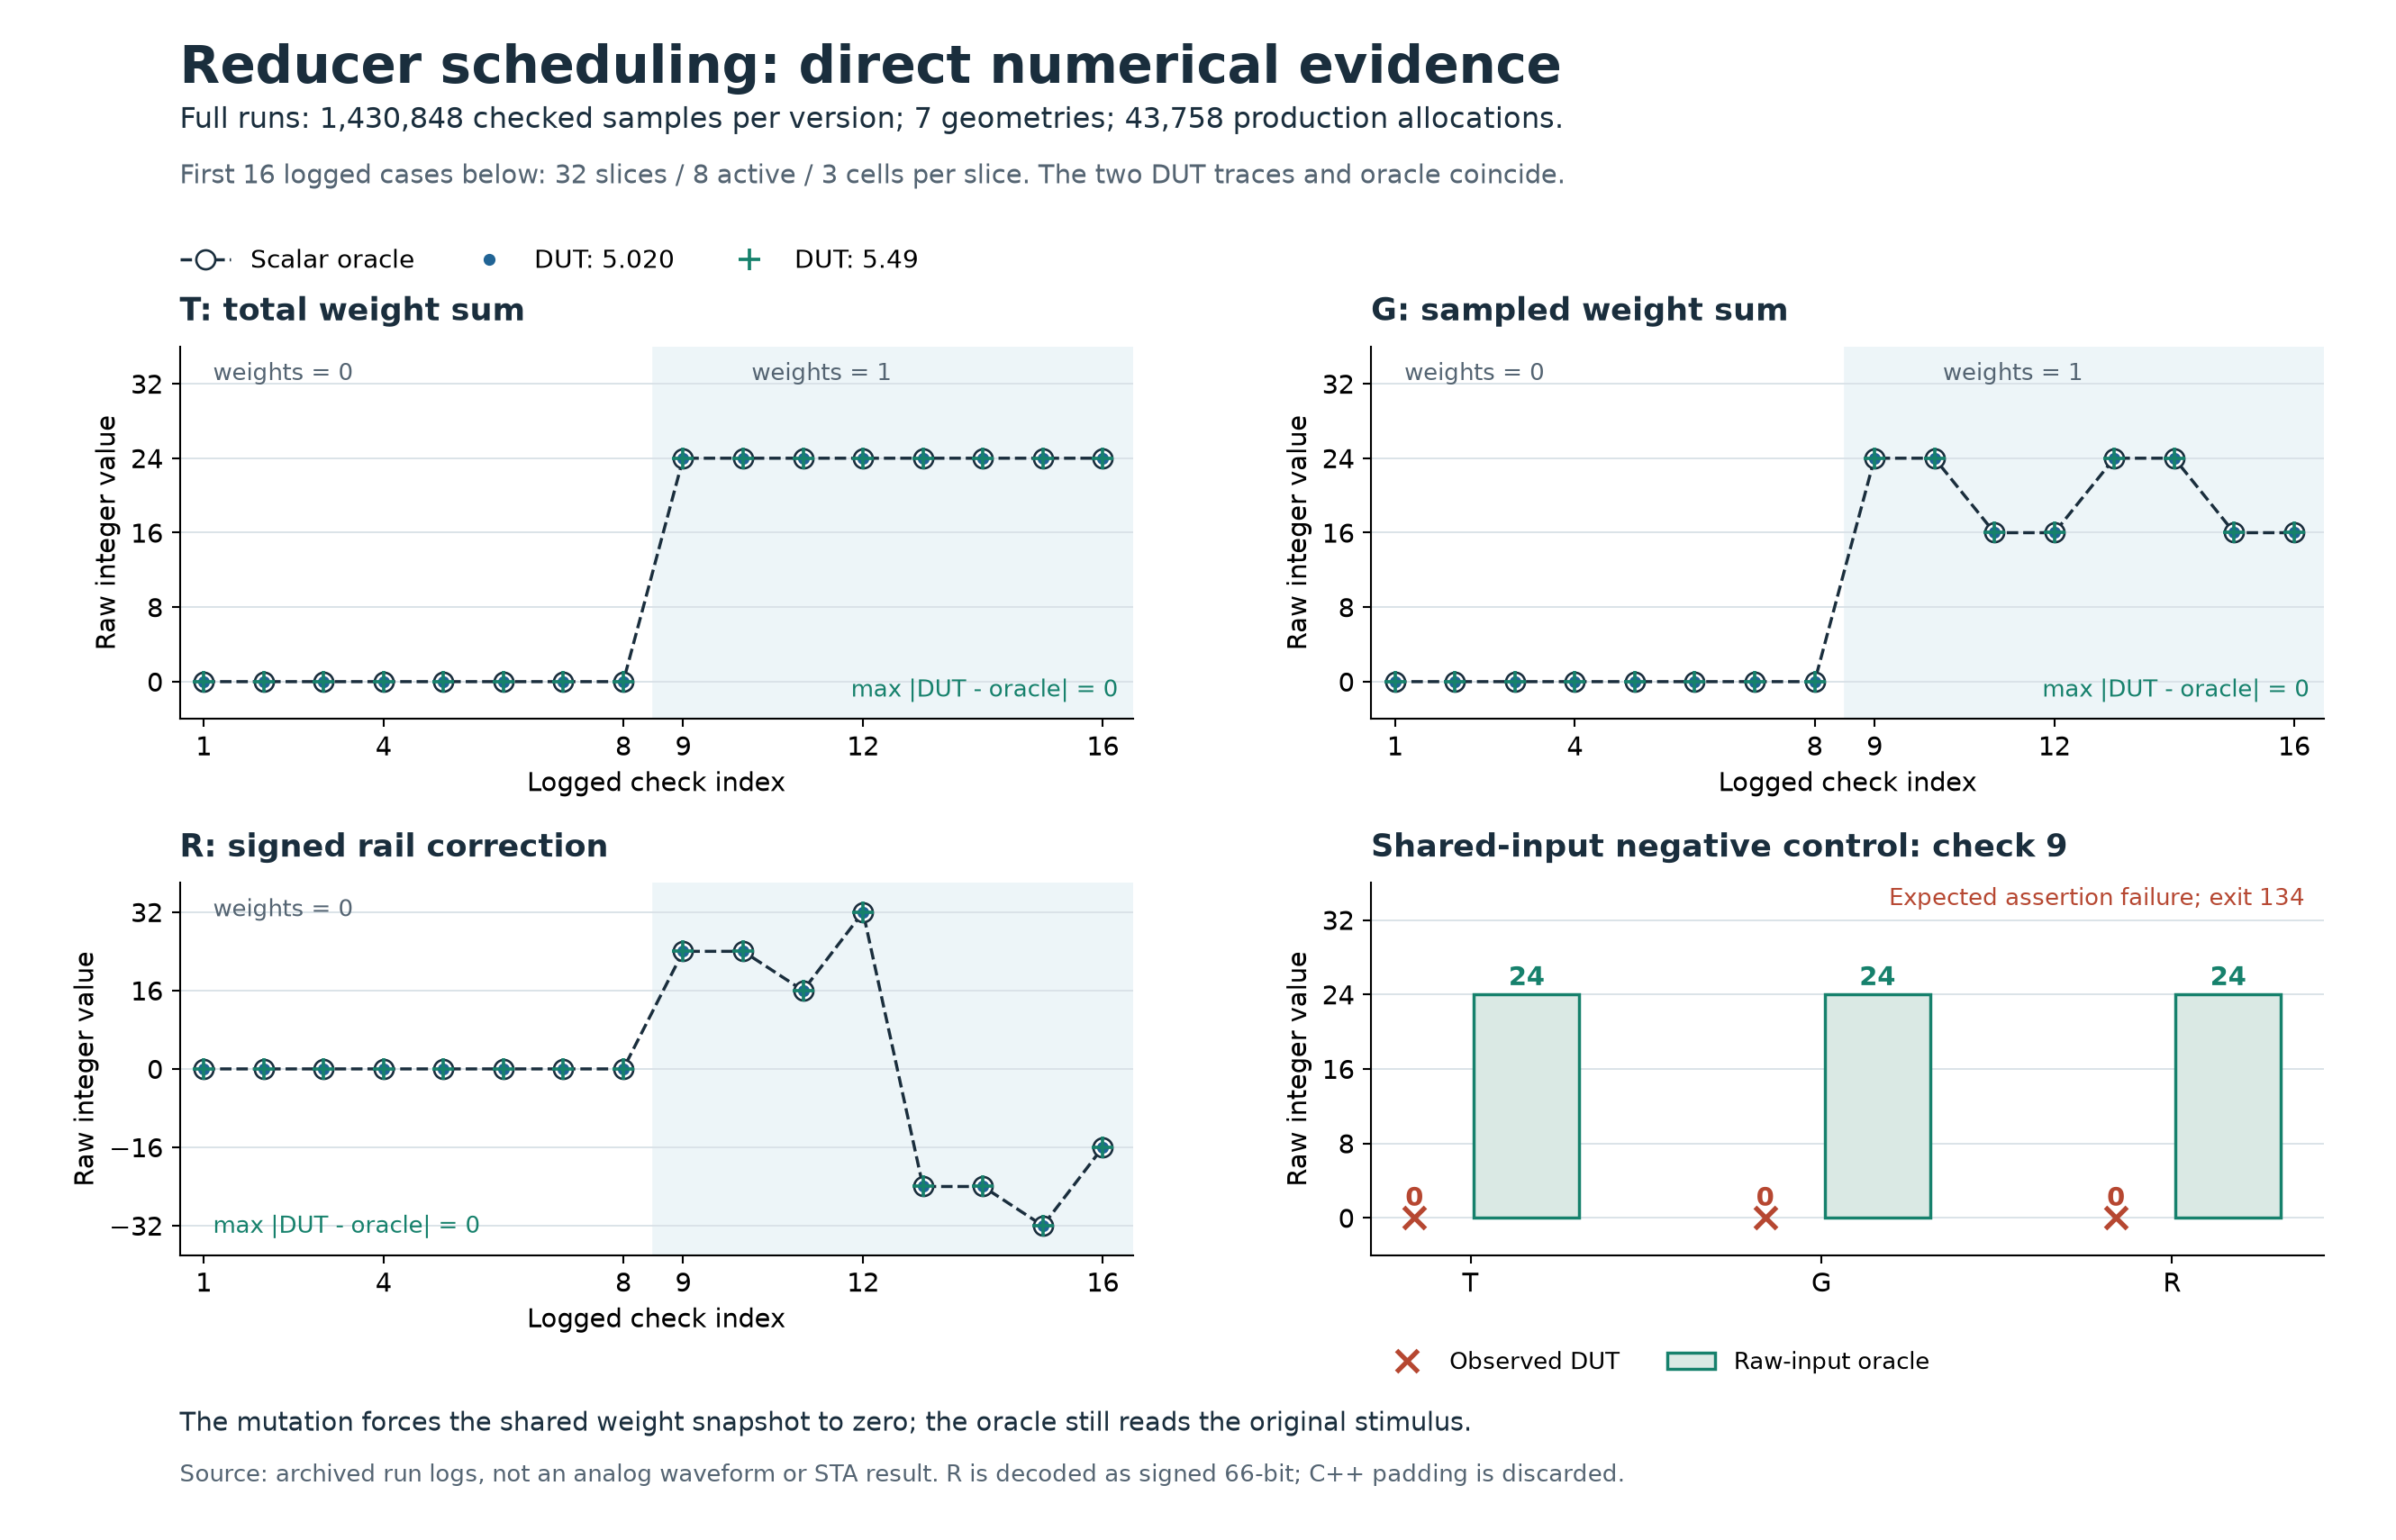
\includegraphics[width=\textwidth]{figures/39_reducer_scheduler.png}
  \caption{归约验证中的数值证据与共同错误负对照。前三个面板仅绘制32个物理slice、8个活动slice、每slice含3个单元这一配置的前16个日志检查点；两个工具版本的DUT结果与逐物理单元的独立参考在这些点重合。完整回归在每个工具版本下分别检查1,430,848个样本，覆盖7种几何配置及43,758个生产分配组合，不能把两次工具运行的数量相加当作额外覆盖。右下角将双方共用的权重快照故意清零，原始刺激参考仍为24，在第9个检查点被断言检出。横轴是检查序号，图中没有重建模拟波形，也没有给出静态时序结论。}
  \label{fig:reducer-scheduler-evidence}
\end{figure}


\subsection{Python 位级镜像的宽度同步}

同一提交的 Python CI 还正确发现另一类问题：生产除法器的余数宽度已改为
\(W_R=P_{W_A}\)，位级镜像却仍使用 \(\max(P_{W_A},P_{W_D})+1\)。
修复同步了宽度、高位分母分类和 \(W_R+1\) 位借位减法，保留原有反漂移门禁。
新增六种小几何共枚举 55,432 个输入对，包含 308 个零分母、31,744 个高位分母分类用例，
以及最负数、非整除的展开 padding；25 项镜像测试全部通过。
本地非 slow Python 回归执行 \code{PYTHONPATH=$PWD/src python -m pytest -m "not slow" -q}，
日志记录 918 项通过、3 项未被选入，用时 678.00 s。
该次收集之后新增的完整顶层映射流程测试另行验证，不能据此把 918 称为当前全部测试数。
证据位于本地实验目录 \code{sar_adc_vivado_20260930/python_regression/manifest.json}；
其原始日志摘要为 \code{82fad3175aa905eac17a80e78fe4a0f98b74f7fe779808225b75373e913bfc74}。
六个小几何的独立复核及 25 项镜像测试另见同一实验目录的
\code{full_mapped_flow_checks/mirror_independent_review.json}。
镜像用例、Python 测试与 RTL 向量有不同计数单位，也有重叠的回归范围，
不能将它们相加为覆盖率或替代最终 GitHub 提交的 CI 状态。

\section{未来动态性能验证应怎样接入}
数字重构修复完成后，可把真实行为模型或混合信号仿真的连续输出导入 ADC 指标工具。但输入必须含均匀采样时间或明确的缺样记录，且剔除启动阶段的方法事先规定。发生错误但保留旧码的事务不能悄悄当作正常样本送入 FFT；要报告错误率，并明确频谱是否来自仅成功的连续区间。

对每个动态场景，至少保留输入频率/幅度、采样率、样本数、窗函数或相干关系、去直流规则、谐波归类、噪声积分带宽与结果单位。对比校准开关时保持相同输入和模拟失配实现，避免把两次随机噪声差异误判为校准收益。时间交织和 DEM 的周期还会产生特定离散 spur，不能只观察最大谐波附近几个 bin。

静态验证应包括端点处理、单调性、漏码和最大局部步长。对 20-bit 全码域，扫过理想整数输入并得到相同数字输出是一个有用的映射测试，但不等同于用连续模拟输入测出所有真实转换阈值。实际模拟非线性、比较器噪声和建立误差必须出现在刺激到输出的路径中，才能被该实验观察。

\section{交付工件的最小集合}
最终工件按用途保存：源码与约束定义要执行的设计；原始日志与 status 文件记录工具实际行为；manifest 和 SHA 将两者绑定；图和报告解释结果。图的像素文件不应成为唯一证据，因为读者无法从图中复原全部码值和异常序列。对于体积较大的 DCP 或完整波形，可以保留在本地实验目录，并在公开仓库中放哈希、生成命令和精简文本报告。

原始失败工件应保留，后续更正通过独立 reviewed result 说明它为何失效。本轮 Windows Vivado 的外层批处理返回 0，而 Tcl status 明确指出负 WNS；这需要区分 raw return code 与归一后的时序结果。随后发现的无驱动又否定了该网表的功能完整性，因此最终状态必须进一步降级为无效综合诊断样本。按时间覆盖原 manifest 会抹去这条发现链，降低可追溯性。

这套组织方法的目的，是让另一位工程师从提交和命令重新得到相同的通过或失败结论，而不是只相信报告作者的描述。对当前工作，功能等价、综合完整性和时序闭合分别列为独立验收项；任何一项未完成，都不得用另外两项的成功替代。

% CI head 417f261 / tested merge 63e9887: RTL job succeeds; workflow conclusion remains separate.
% Preceding local 169f, failed-job 0c4a and successful-job f028 artifacts are retained under history/.
\section{成功 RTL job 的 22 项图证与独立算术验收}
\label{sec:historical-21-evidence}
\label{sec:ci-21-evidence}
\label{sec:ci-22-evidence}
本节四幅图改用 \code{docs/evidence/20260930/ci_rtl_417f/} 的真实 CI 日志。
\textbf{22 项 RTL bench、3 类严格 lint 和独立算术审计均通过，本次 RTL job 的结论为 success。}
归档抓取时 workflow 仍为 \code{in_progress}，不能由一个 job 成功推断整个 workflow 全绿。
归档 head 为 \code{417f261}，实际测试 merge 为 \code{63e9887}，两者完整 Git tree 均为 \code{f0be3b81}…；26 项生产 RTL 的内容摘要为 \code{1e3fab94b7b2}…。
本次是已发布行和缓存候选结构的 RTL 功能验收，包含新增缓存装载测试及缓存消费路径；实际综合、布局布线和门级结果仍按各自实验记录判定。
制图器核验归档清单、日志、步骤结论以及 head 中 88 项输入的实际字节，不用当前工作树替代历史输入。
样本、输入码、断言和检查节拍分别保留单位，不相加为覆盖率。

\begin{figure}[H]\centering
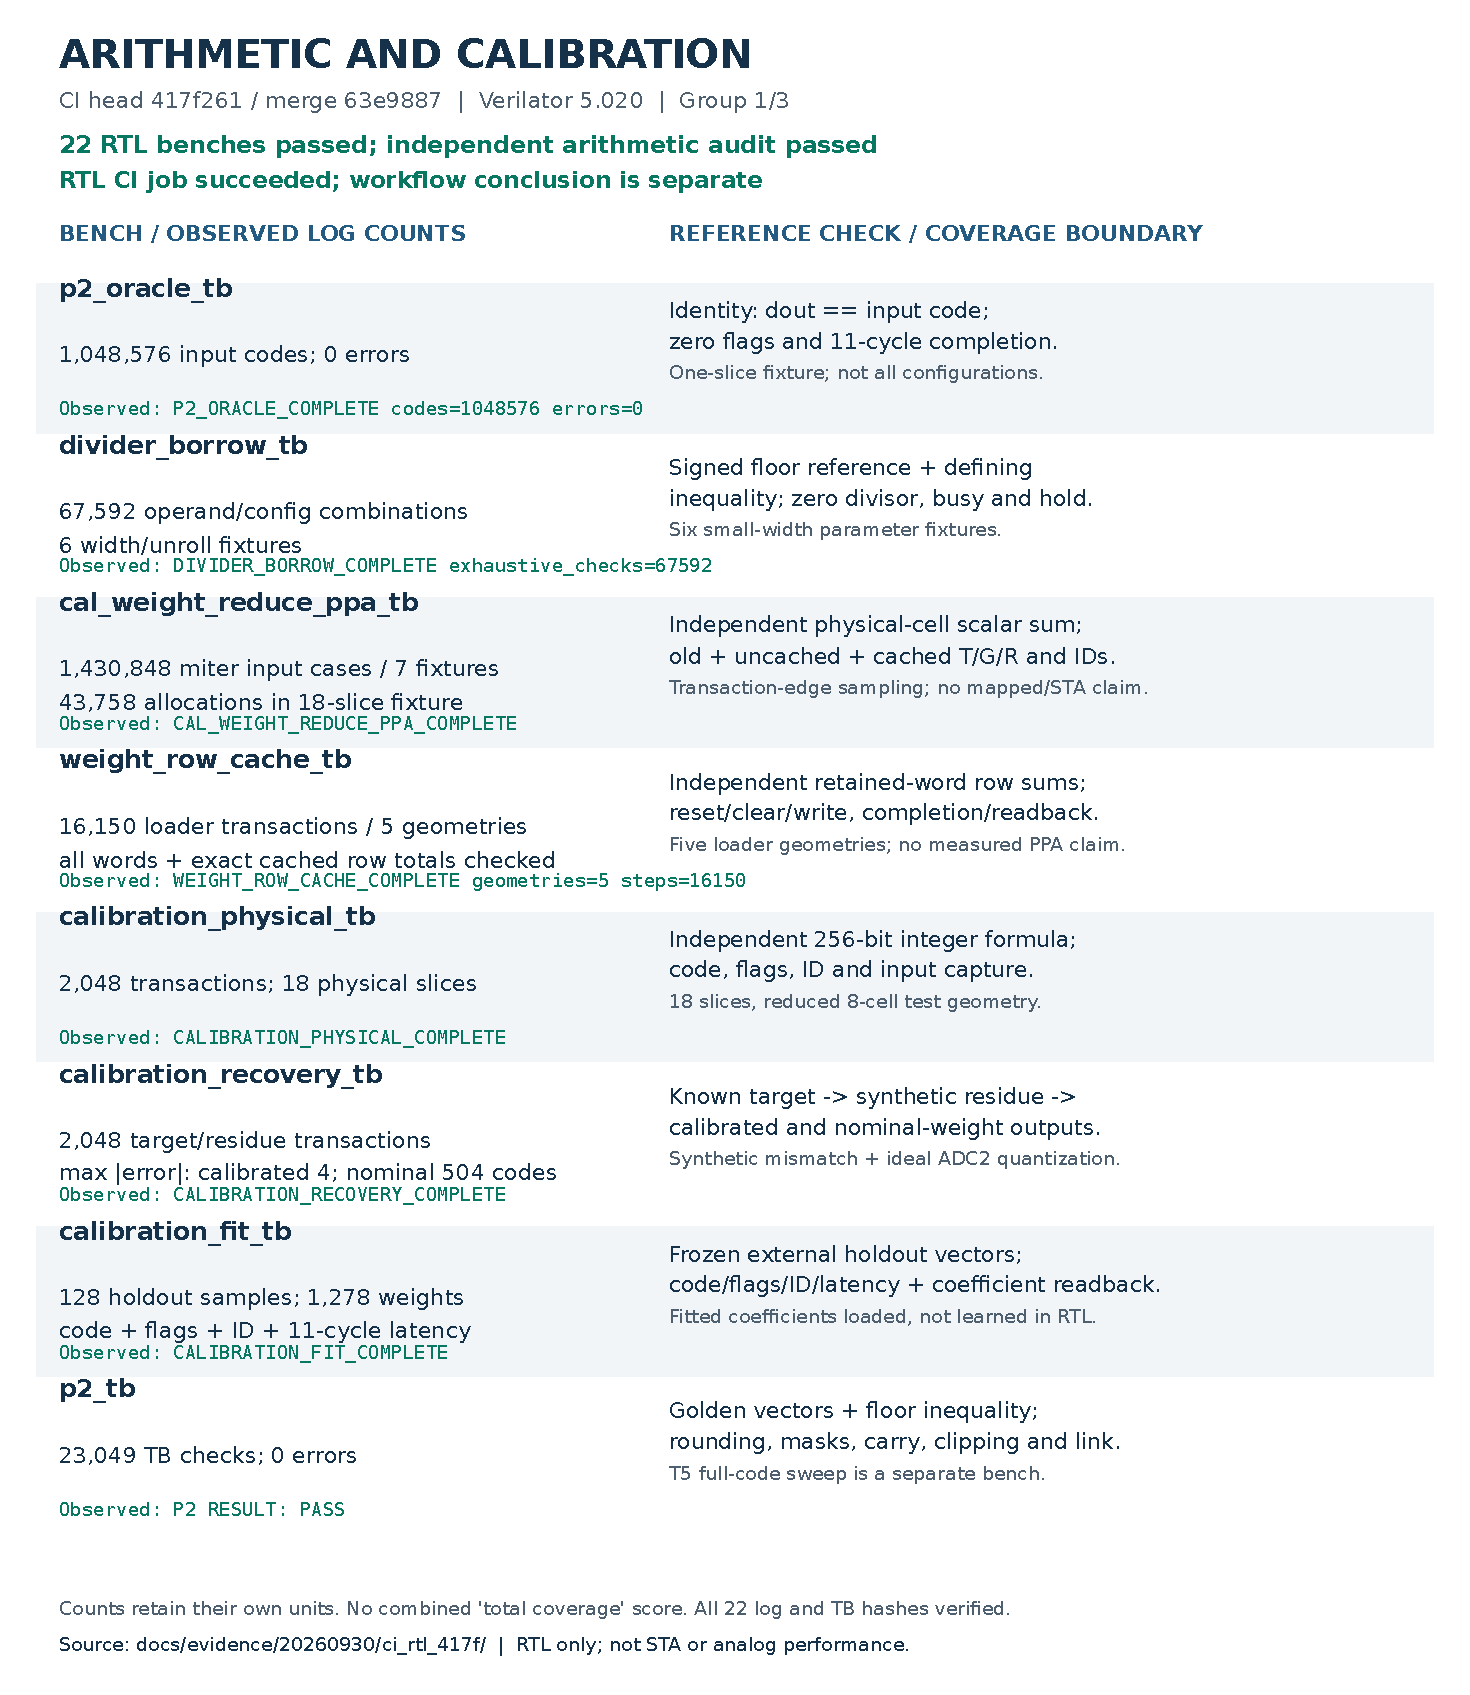
\includegraphics[width=.96\textwidth]{figures/final_regression_arithmetic.pdf}
\caption{本次 CI 中算术与校准的八项 RTL 回归。归约器将旧实现、未缓存实现和缓存实现逐笔对照独立物理单元 scalar 求和；新增装载器检查独立保留字、缓存行和与读回；另行执行并通过的独立算术审计在本节后部说明。全码恒等和除法穷举分别受简化配置及六组小位宽的范围限制。}
\label{fig:final-regression-arithmetic}
\end{figure}

\subsection{事务、取消与结构调度}
图\ref{fig:final-regression-protocol}中的结构顶层 P7 检查 438 笔输出及其延迟、7,680 个协议节拍。
本次 CI 另以 \code{recon_ppa_latency_tb} 在 P5/P6/P7 各连续启动 32 笔，间隔 16 拍，验证输出延迟 15/13/11 拍、busy 释放 14/12/10 拍；不是旧 \code{final_profiles/} 日志。
\code{review_recon_protocol_tb} 未打印总数；\code{review_top_protocol_tb} 打印 38。

\begin{figure}[H]\centering
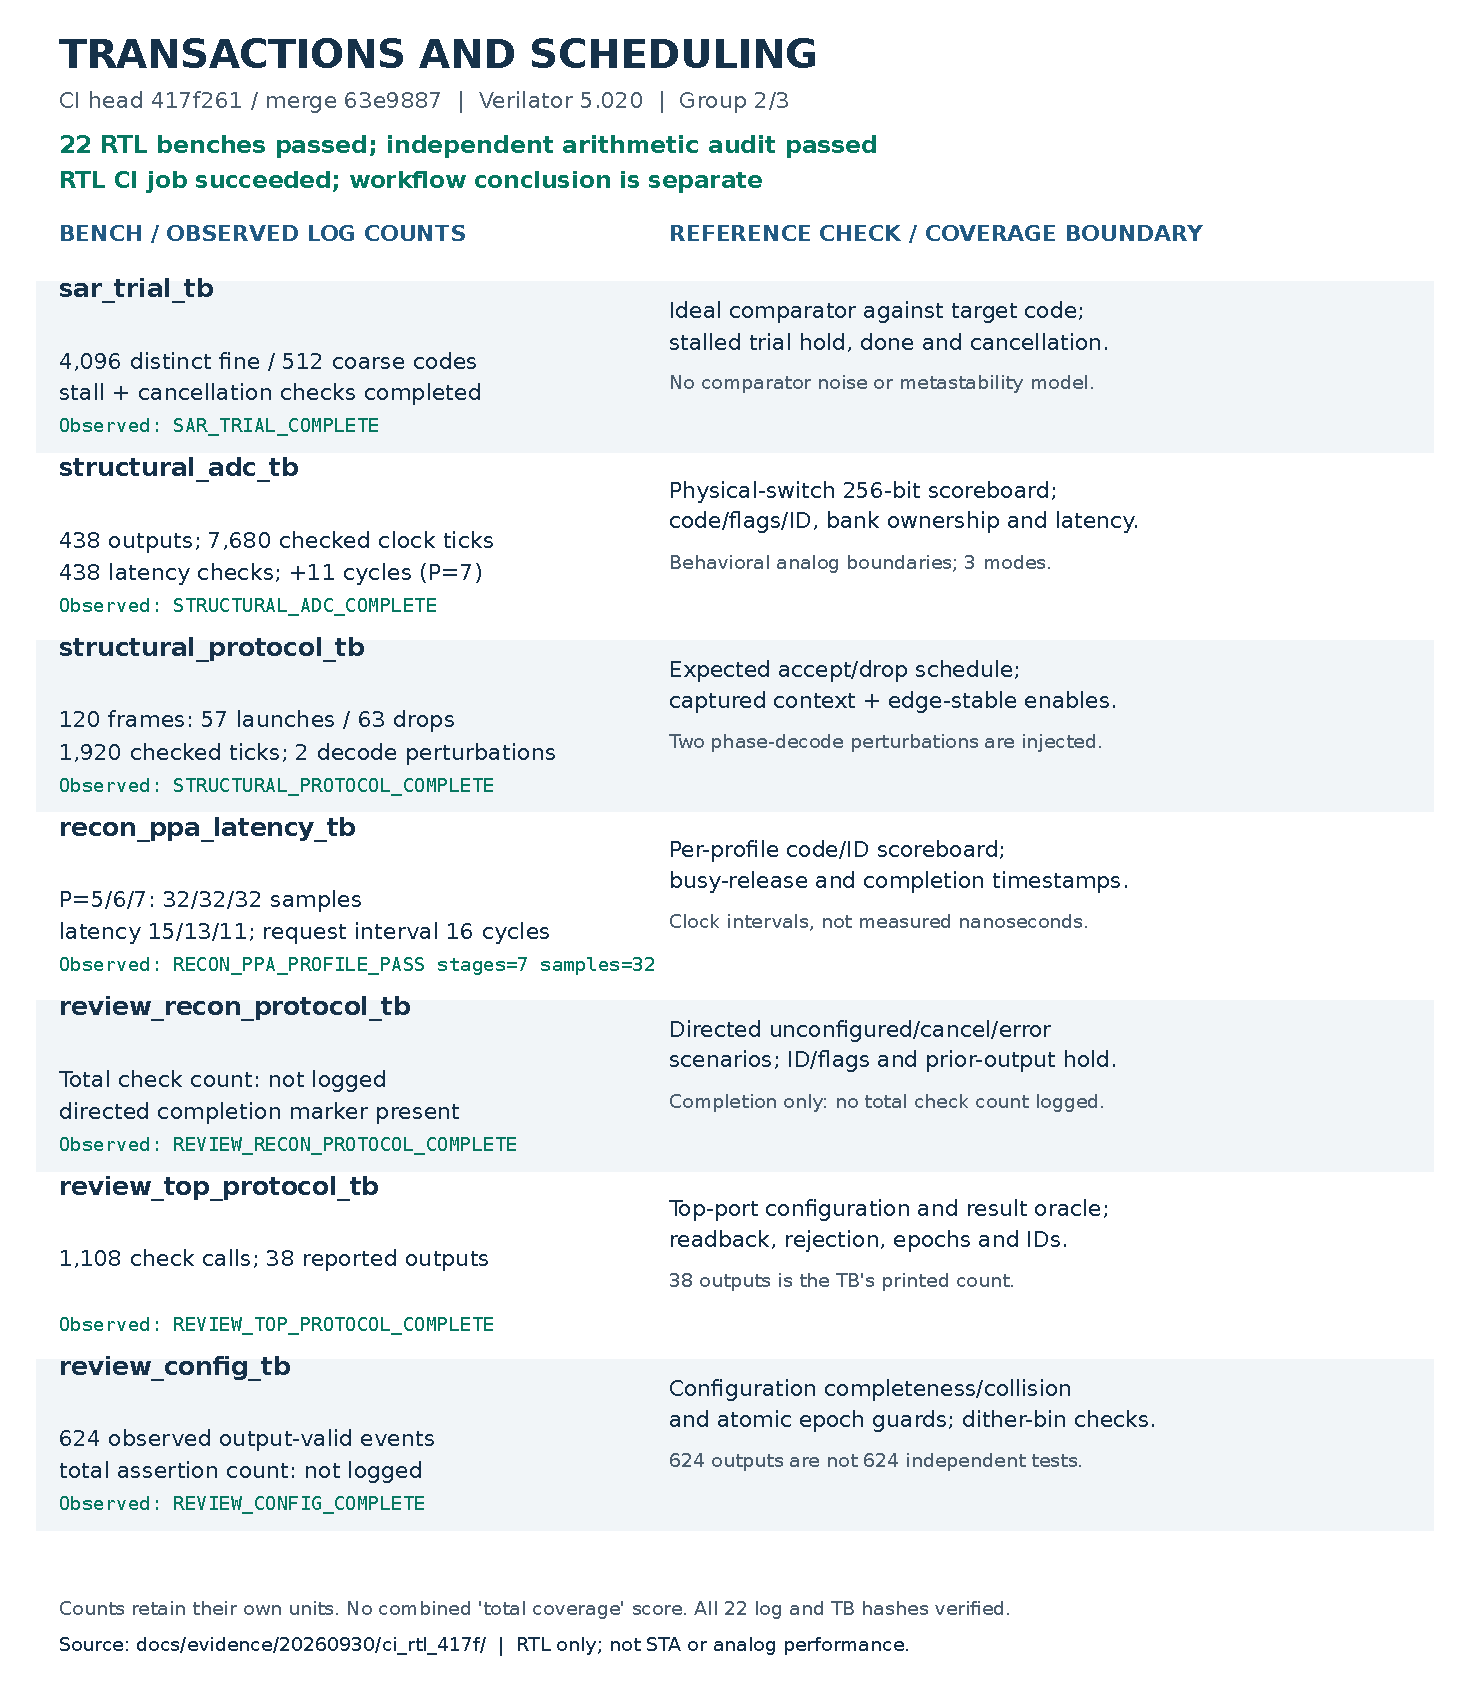
\includegraphics[width=\textwidth]{figures/final_regression_protocol.pdf}
\caption{本次 CI 的七项事务与调度证据，覆盖 SAR 停顿/取消、上下文隔离、ID/flags 对齐、配置屏蔽和 epoch 取消。图中为功能时钟间隔，不是门级纳秒延迟或 640\,MHz 时序签核。}
\label{fig:final-regression-protocol}
\end{figure}

\subsection{基础模块、配置和兼容顶层}
图\ref{fig:final-regression-system}保留每个测试原有计数器的含义。
外设各小计是累计值；dither 的七种条件分别在 200,000 个观测周期内接收 196,866 或 200,000 笔输出。
\code{tree_mapping_tb} 在此次 CI 中是 Verilator RTL 运行，不能改称真实网表仿真。

\begin{figure}[H]\centering
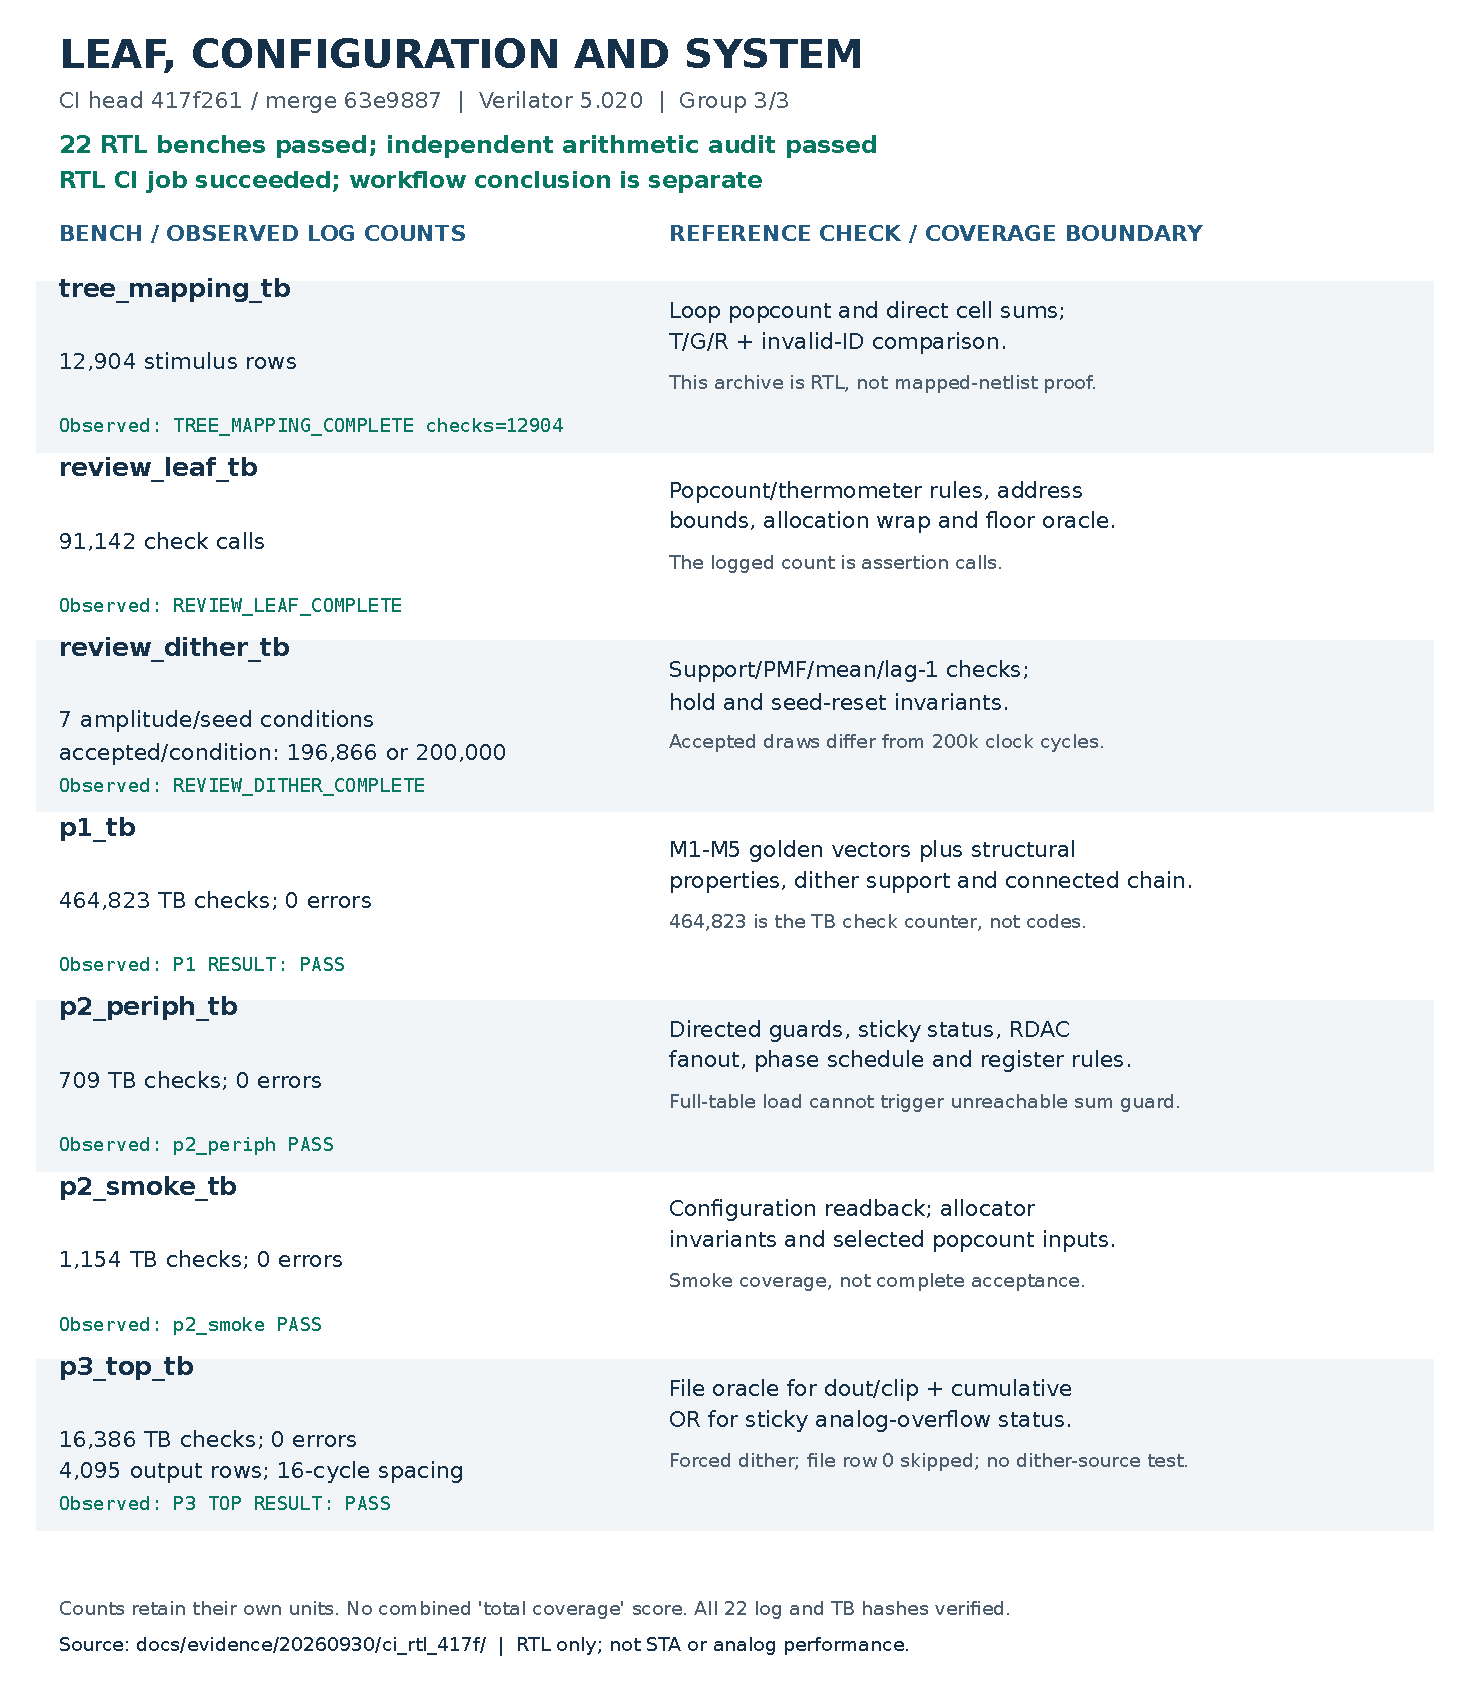
\includegraphics[width=\textwidth]{figures/final_regression_system.pdf}
\caption{本次 CI 中基础模块、配置与兼容顶层的七项证据。兼容顶层比较 4,095 行输出，跳过向量第 0 行，并 force 注入 dither；因此不覆盖该模式下片内 dither 源。analog-overflow 仍按累计 OR 的粘滞语义比较。}
\label{fig:final-regression-system}
\end{figure}

\subsection{新日志中的定量观测}
图\ref{fig:final-regression-quantitative}的 A、B 面板读取本次 CI 全部 128 条 \code{FIT_ROW}：码值、flags、ID 均相符，延迟均为 11 拍。
横轴是留出样本序号；这些数据来自外部拟合系数的加载和重构，并不是片上参数学习或模拟瞬态测量。
C 面板只有日志记录的两项最大绝对误差：标称权重 504 码、校正权重 4 码，不由两根柱子推导 RMS、SNDR 或 ENOB。

\begin{figure}[H]\centering
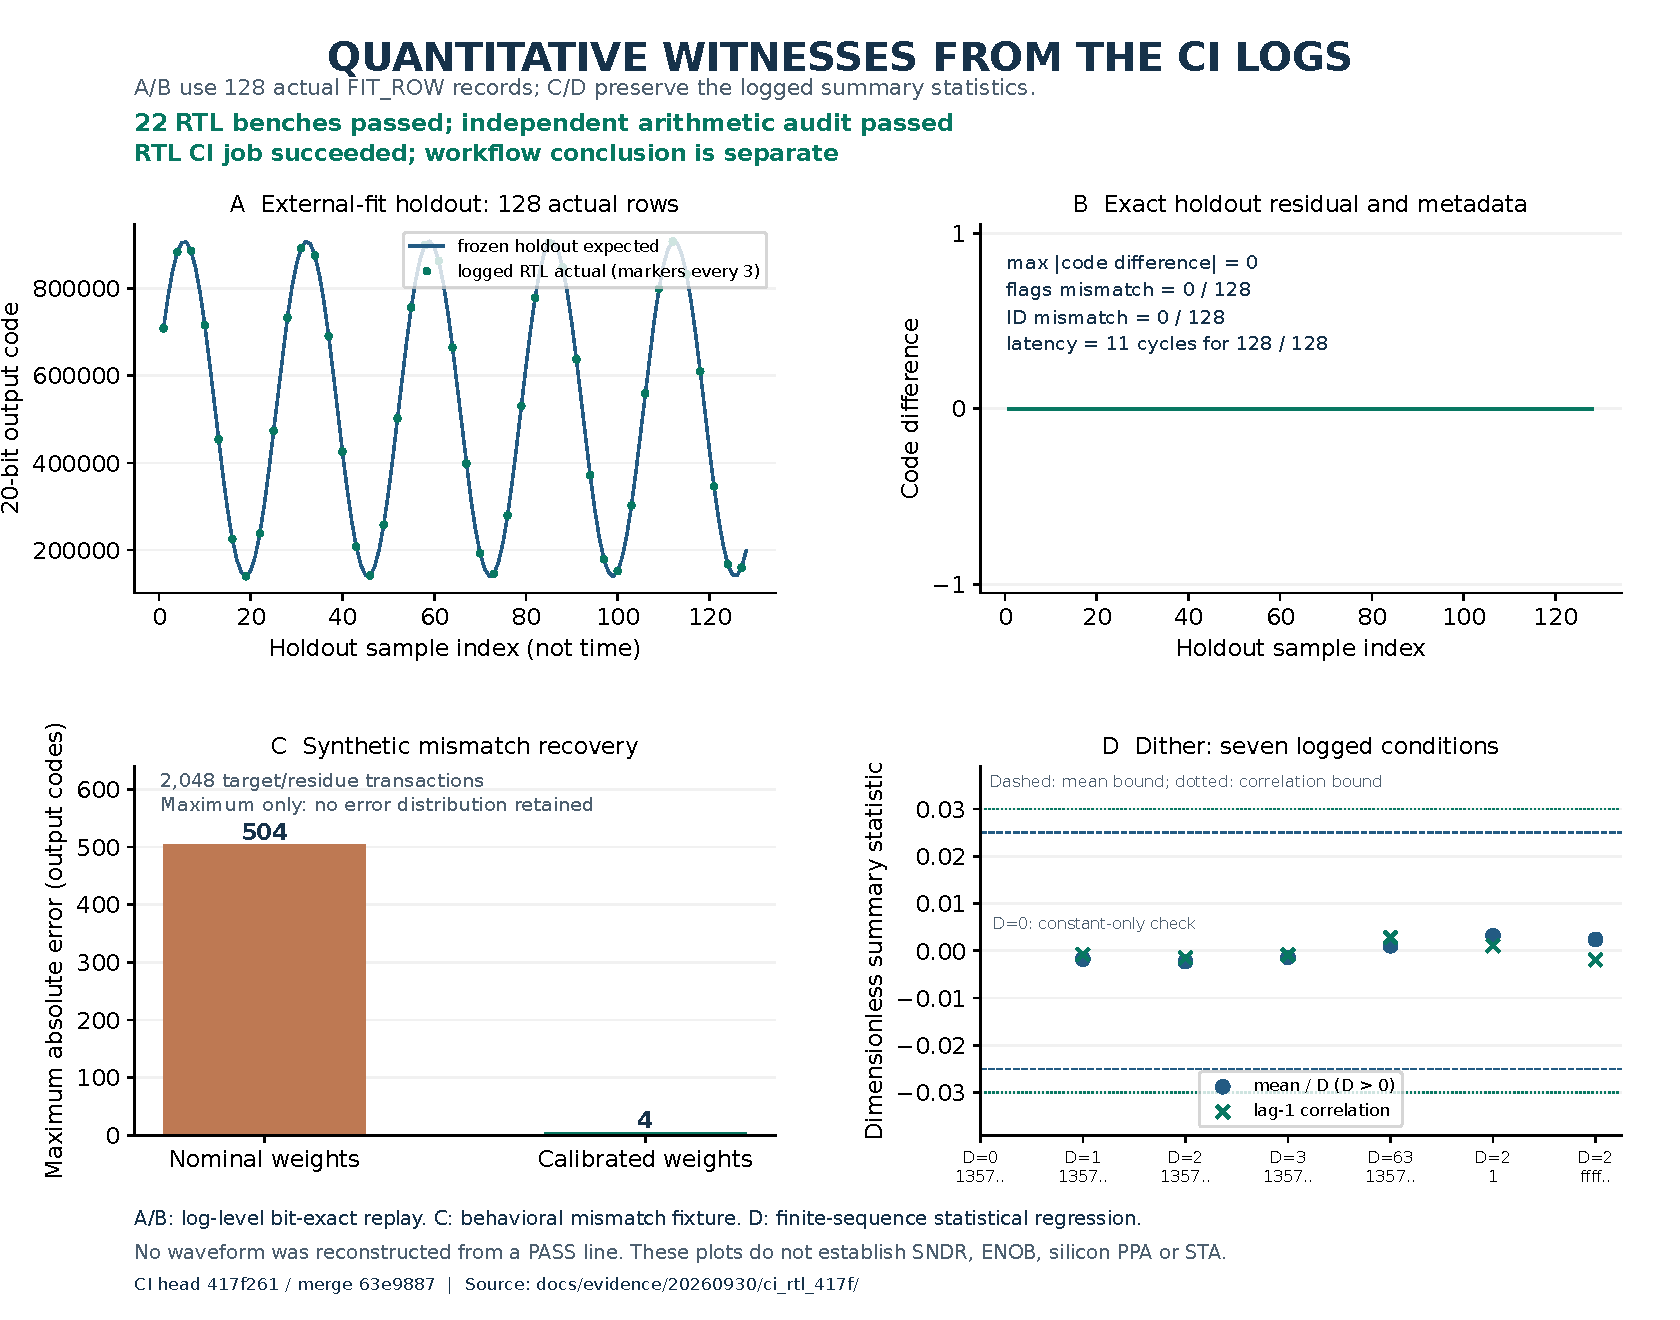
\includegraphics[width=\textwidth]{figures/final_regression_quantitative.pdf}
\caption{本次 CI 日志的实际数值。A/B 为 128 笔留出数据；C 为 2,048 笔合成失配的最大误差摘要；D 为七组 dither 的打印统计量，均值除以幅度 $D$，门限分别为 $\pm0.025$ 与 $\pm0.03$。$D=0$ 方差为零，相关性不计算，也不画成有效零值。}
\label{fig:final-regression-quantitative}
\end{figure}

D 面板均值/相关性只保留日志的六位小数。原日志没有各 PMF bin，因此不能补画分布；其余三图使用证据矩阵，不从完成标记伪造波形。
归约器参考计算和判据位于该 head 的 \code{sim/tb/cal_weight_reduce_ppa_tb.sv:63} 至 118 行：独立 scalar 函数读取原始刺激，同时验证旧实现、未缓存实现和缓存实现的 \(T,G,R\) 与非法地址标志。
本次 5.020 CI 完成七种几何、1,430,848 次检查；每种几何的日志均记录 \code{cache=1}，43,758 个生产分配组合包含在这些检查中。
新增 \code{weight_row_cache_tb} 对五种几何完成 16,150 个事务步，按独立保存的各权重字求和，逐步检查缓存行和、存储字、由独立装载位图计算的 complete 状态与地址读回，包含 reset、clear 和写入同沿的优先级场景。
该缓存测试不是将归约器 1,430,848 个组合重复计数；本地双工具的最大值、clear 后替换和负控仍保留图\ref{fig:row-cache-evidence}的独立来源。
另外的本地双版本复验与共同错误负控仍按图\ref{fig:reducer-scheduler-evidence}的原来源保留。

\subsection{独立算术审计：CI 成功与本地双版本负控}
历史 \code{0c4a772} CI 的独立审计未进入仿真：runner 将头文件安装目录设置为 \code{VERILATOR_ROOT}，使已安装启动器寻找不存在的 \code{verilator_bin}，以 127 返回。
该失败仍保留于旧 \code{ci_rtl_0c4a/arithmetic_entry_failure.log}；不得因后续修复而覆盖其失败状态。

\begingroup\raggedright
随后修复启动路径，并处理本机 5.020 暴露的文件刺激调度问题，形成独立归档 \code{docs/evidence/20260930/arithmetic_runner_ci/}。
两种记录的工具版本分别完整通过 40,010 项 MAC（其中 20,859 项不溢出）、40,000 项 ADC2、10,048 笔除法和 8 组 flags 序列。
保持陈旧 MAC 输入和固定 ADC 输入的两个负控分别在 MAC 第 3 行、ADC 第 2 行失败；另有 8 项路径/环境单测通过。
这些本地结果保持生产 RTL 和期望向量不变，但修复了审计 runner 和 TB，不能倒写为 \code{0c4a772} 的独立审计通过。
本次 \code{417f261} 在 Ubuntu/Verilator 5.020 上也完成同样的独立审计，
真实日志与 manifest 位于 \code{ci_rtl_417f/arithmetic-audit/}，七项受检源文件与被测 Git tree 一致。
本次 RTL job \code{109627112125} 完整成功；该归档时 workflow \code{36633152469} 尚在运行，原记录保持不变。随后单独取得的 \code{ci_workflow_417f/} 确认本次同一head的9个job全部成功；其Python、完整验收和确定性结论分别按该新归档判断，不能从旧 \code{ci_workflow_f028/} 移用。\par\endgroup

\begin{figure}[htbp]\centering
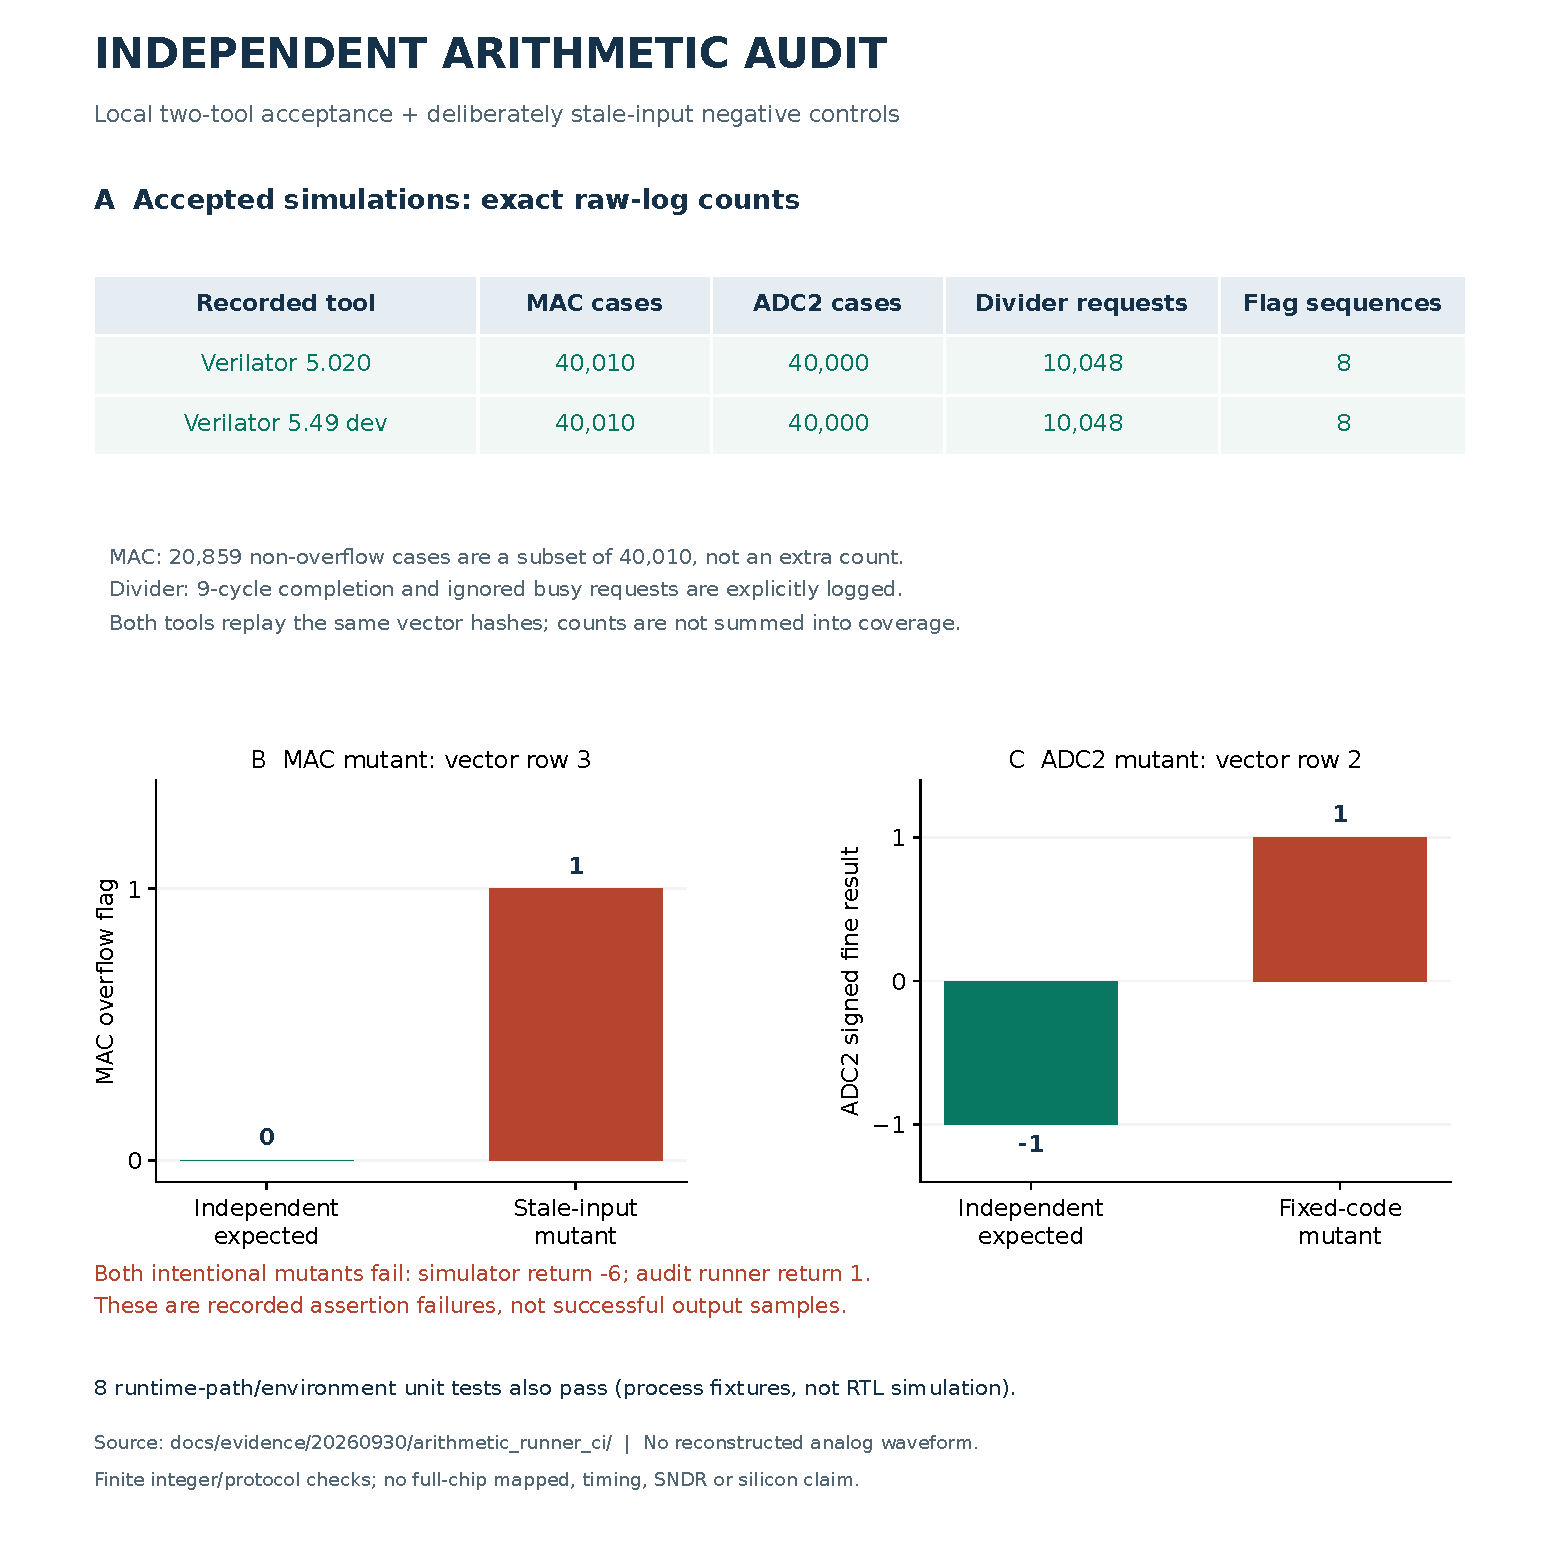
\includegraphics[width=.97\textwidth]{figures/arithmetic_runner_dual_tool.pdf}
\caption{独立算术审计的本地双版本正、负控。上表为各版本原日志的精确计数，20,859 项不溢出 MAC 是 40,010 项的子集。下图只绘制真实失败行：陈旧 MAC 输入使第 3 行溢出标志由期望 0 变为 1；固定 ADC 输入使第 2 行有符号细码由期望 $-1$ 变为 $+1$。两个变异均被独立期望值检出；图不重建波形，也不把负控失败计为正常样本。}
\label{fig:arithmetic-runner-dual-tool}
\end{figure}

\begingroup\raggedright
图\ref{fig:arithmetic-runner-dual-tool} 的脚本为 \code{audit_figures/make_arithmetic_runner_evidence.py}，
来源及数值见 \code{audit_figures/arithmetic_runner_dual_tool.sha256.json}。
两种本地工具重播同一组向量；本次 CI 是另一环境复验，各次计数不相加为更大的输入覆盖集合。\par\endgroup

\subsection{重建入口与历史保留}
在报告目录执行 \code{python audit_figures/make_final_regression_evidence.py --schema ci} 可重建四张 PNG/PDF。
脚本校验 CI archive 的 \code{sha256.json}，核对步骤而非仅看 job 总状态，逐字节读取 Git head 中的输入，核对 26 项生产 RTL 集合与 22 份日志，再解析数值和唯一完成标记。
每张同名 \code{audit_figures/final_regression_*.sha256.json} 保存上述来源、测试台行号、图件和脚本摘要；本次 \code{tested_inputs_sha256.json} 摘要为
\par\noindent\code{a265a71f9981d137d2cd763e7341e2c7992c2280bf61ab0111a1a85a2726be33}。

旧 169f 图、PDF、脚本、分节和哈希记录逐字节保留在
\code{history/final_regression_169f_before_ci_0c4a/}，由该目录 \code{archive_manifest.json} 校验。旧 \code{0c4a} CI 的四图、脚本、分节、检查与摘要另存于 \code{history/final_regression_ci_0c4a_before_f028/}；f028 成功 RTL job 的四图、脚本、分节和摘要保存在 \code{history/final_regression_ci_f028_before_417f/}。原仓库旧证据没有被覆盖。
图件 \code{31_divider_profiles.png} 仍是旧 \code{fd885e882ad5}… 快照的 compact 三档生产顶层实跑，每档 438 次输出与延迟检查，不能与本次各 32 笔的连续启动夹具混成一次实验。
本节没有启动新仿真或 EDA，全部图只重建已归档的日志；不提供模拟电路、STA 或硅片性能签核。


\chapter{综合、时序与下一阶段实施}
\section{平台验收口径}
用户已明确确认：640\,MHz 保留为 ASIC 目标；Virtex-7 FPGA 按实测可实现频率验证，并独立报告与目标的差距。FPGA 每 16 拍接收一笔样本的名义速率为 \(f_{\rm clk}/16\)，不能在较低 FPGA 时钟下仍沿用 40\,MS/s 标签。OOC 实现的外部时钟和 IO 为指定上下文假设，尚不能替代整板 IO、模拟宏和目标 ASIC 工艺签核。

\section{当前主要硬件风险}
\begin{enumerate}
\item \textbf{权重存储和宽并行读：}接口容量为18$\times$71$\times$48=61,344 bit，全表并行可见。合法权重的最高位恒零，显式掩码后只有60,066个系数数据位可能变化；行和缓存另增加18$\times$54=972个状态位，装载完整性位和其他控制状态另计。以上是源码位数，实际FF数以综合为准。窄掩码到物理行的改写减少了宽18:1选择的源码路径，但带来了更多零门控叶子。普通SRAM很难直接提供同拍568项读取，不能仅凭RTL数组语法判定存储映射与面积。
\item \textbf{组合关键路径：}同拍物理权重归约、带符号 64-bit 乘法、132-bit 容器中的加减与边界比较，随后迭代除法每拍串接 7 级试减与余数选择。修复版默认采用63-bit余数和64-bit借位差，复用一次减法的借位；原实现的比较加减法不能继续当作当前结构。\code{P_STAGES=7} 是每拍展开数，不是 7 级流水。令每拍展开数为 \(p\)，当 \(p=7,6,5\) 时，\(\lceil63/p\rceil+2\) 分别为 11、13、15 拍；三种配置的 \code{busy} 释放及下一笔启动已由历史参数回归验证。小于 5 的配置已被顶层参数守卫拒绝。
\item \textbf{频率：}16 相位$\times$40\,MS/s 要求 640\,MHz，即 1.5625\,ns 周期；代码能仿真并不说明在 40\,nm、指定 PVT 和真实布线后能满足。10\,ns 约束对应仅 6.25\,MS/s 的数字节拍。
\item \textbf{模拟边界：}Flash、两路粗比较器、后级比较器、RDAC、RA、参考、AUX、TP 同步都缺真实时序/幅值约束；比较器数据未经异步握手 CDC 证明。现有相位规划若无法在模拟建立预算内闭合，须改时序或并行化，不应通过放宽约束仍保留 40\,MS/s 标签。
\end{enumerate}

\section{可执行的工程化里程碑}
\begin{longtable}{>{\raggedright\arraybackslash}p{12mm}>{\raggedright\arraybackslash}p{54mm}>{\raggedright\arraybackslash}p{86mm}}\toprule 优先级&实施项&客观验收准则\\\midrule\endfirsthead\toprule 优先级&实施项&客观验收准则\\\midrule\endhead
P0&冻结当前 RTL/参数/向量/测试工具哈希，配置导入增加 epoch 与排列校验；补专利 [12] 差距 issue。&权重读回与加载镜像逐项一致；跨样本 ID/epoch 不错配；issue 含 claim 1 每一限定与接口设计。\\
P0&校准算术形式化/约束随机：极端合法权重、\(G=0\)、重复 ID、负商、半值向偶、溢出上下边界。&独立任意精度 oracle 位精确；输出码、flags、hold、valid、ID 全部逐笔一致。\\
P1&规划权重 bank、配置期聚合及归约流水；对当前结构与候选结构分别综合。&相同库、角、约束下四个单元及顶层的面积、关键路径、存储映射、功耗活动假设、网表可复现；功能逐位等价。\\
P1&模拟宏接口契约：TP/AZ/参考/AUX/比较器 valid 的 setup/hold、非重叠、最大建立误差与电压域。&Spectre/AMS 瞬态及 PVT 含最坏码跳变；每个接口量有预算与测量波形。\\
P1&明确 [12] tracking 属于专利覆盖差距，并确认目标架构是否采用；若采用再增加最新码寄存、来源 ID 和有效性。&双通道交叉激励证明因果更新；迟到码、丢码、复位/clear 不污染下一样本。\\
P2&数字顶层 DC/等价/STA 与混合信号协同闭环。&1.5625\,ns 目标下 setup/hold、未约束端点、组合环、锁存器、DRC、PVT 和功耗报告齐全；否则正式降级吞吐规格。\\
P2&最终系统级 SNR/DR、SNDR、SFDR、INL/DNL、温漂及输入带宽。&从连续时间或晶体管/硅片数据提取，报告采样数、窗函数、频率、置信界和原始数据；不能复用数字 testbench 指标。\\
\bottomrule\end{longtable}

\section{面向综合的保守优化顺序}
先用当前 RTL 在同一目标工艺和真实 SDC 建立基线，分别报告 权重存储、权重归约、残差乘加、除法器和集成顶层，确认最差路径究竟在权重选择、归约、乘法还是除法。随后只改一个瓶颈：若前端归约为主，优先配置期预聚合、物理行局部和、有限级流水；若宽乘法为主，先形式证明合法输入的紧位宽，再缩小乘数；若除法为主，比较分块流水、并行除法器或“倒数近似 + 逐位精确修正”。每次优化都必须保留 \(\lfloor\cdot\rfloor\)、溢出边界和逐样本标记，验证 initiation interval 与 latency 同时满足固定 16 相位。面向高频的最终结果必须在布线后 STA 而非 RTL 逻辑深度推测下确认。

Vivado 综合只能提供 FPGA 结构筛选和对应器件下的资源/时序结果。ASIC 的面积、功耗与时序比较必须使用相同标准单元库、PVT 角和约束；FPGA 的 LUT、DSP、BRAM 与时序结果不能替代 40\,nm ASIC 的 PPA 签核。


\section{已实施的面积导向归约改写}
采样dither的第 \(j\) 个轨在所有活跃slice中相同。原先逐单元取正负、再求和，可以在整数精确域内交换顺序：
\begin{align}
C_j &= \sum_{s\in\mathcal A}W_{s,u_j}, & M &= \sum_j C_j,\\
G &= \begin{cases}T-M,&\text{sampling dither开启}\\T,&\text{关闭}\end{cases}, &
R_d &= \begin{cases}\sum_j r_j C_j,&\text{开启}\\0,&\text{关闭}\end{cases}.
\end{align}
\code{cal_weight_reduce.sv} 保留原有 \(T\) 和 \(W_{on}\) 树，并共用物理叶子。新列树先得到4个 \(C_j\)，再做4次条件取负，取代原来的 \(18\times4=72\) 次。没有增加寄存器、额外宽观测口、系数状态或流水拍；没有改变取整、饱和和标志。\(M\) 是 \(T\) 的子集，且原有位宽守卫覆盖全部系数和，因此 \(T-M\) 不发生无符号借位回绕。无效/重复ID仍按原协议报警，而求和位图语义也保持一致。

消除补零节点并共享原设计相同子树后，原先受dither影响的独立gain加法为178个、dither加法为71个；候选为列加法68个、mask汇总3个、轨汇总3个、gain减法1个。该部分加减表达式由249减为75，减少174个；条件取负由72减为4。\textbf{这是源码结构计数，不是LUT、标准单元面积、功耗或频率实测。}新gain多一个末端减法，可能改变关键路径；只有相同库或器件、相同约束的综合对照才能判断实际收益。不能把“表达式少70\%”写成“芯片面积少70\%”。

此处列归约改写本身没有改变61,344 bit的权重接口容量；后续最高位掩码与行和缓存的状态变化在第\ref{ch:synthesis-repair}章单列。当前全表并行读语义不会自动成为单块SRAM。可编程系数、异常范围和16拍启动间隔均保留。除法默认7保持不变，5与6作为可复现候选；不在缺少映射数据时盲目更改默认值。

\section{保持16拍吞吐的三参数实际比较}
前代精简权重版本（内容摘要 \code{fd885e882ad5}）分别以5、6、7展开数运行完整18-slice结构顶层。每种配置均有438笔正确输出、7,680次逐拍检查、438笔真实接受沿到提交沿的延迟检查；三种模式、18个slice均覆盖。证据为 \code{docs/evidence/20260930/compact_profiles/} 下的原始运行日志、manifest和源码摘要，编译与运行退出码均为0。实测输出延迟仍为15、13、11拍。
这一前代 RTL 内容摘要也已在 \code{ci_rtl_0c4a/} 的 \code{recon_ppa_latency_tb} 中重新通过各32笔连续16拍启动检查，busy释放仍为14/12/10拍。该项是缩小阵列的重构夹具；\code{compact_profiles/} 则是18-slice结构顶层的438笔检查。下表的busy与输出拍数由这两种不同范围的实际回归相互核对，不把缩小夹具扩称为完整模拟系统吞吐证明。
\begin{center}\begin{tabular}{rrrrr}\toprule
展开数&除法迭代拍数&busy释放拍&输出提交拍&距下一次请求\\\midrule
5&13&14&15&1拍\\
6&11&12&13&3拍\\
7&9&10&11&5拍\\\bottomrule
\end{tabular}\end{center}
\begin{figure}[H]\centering
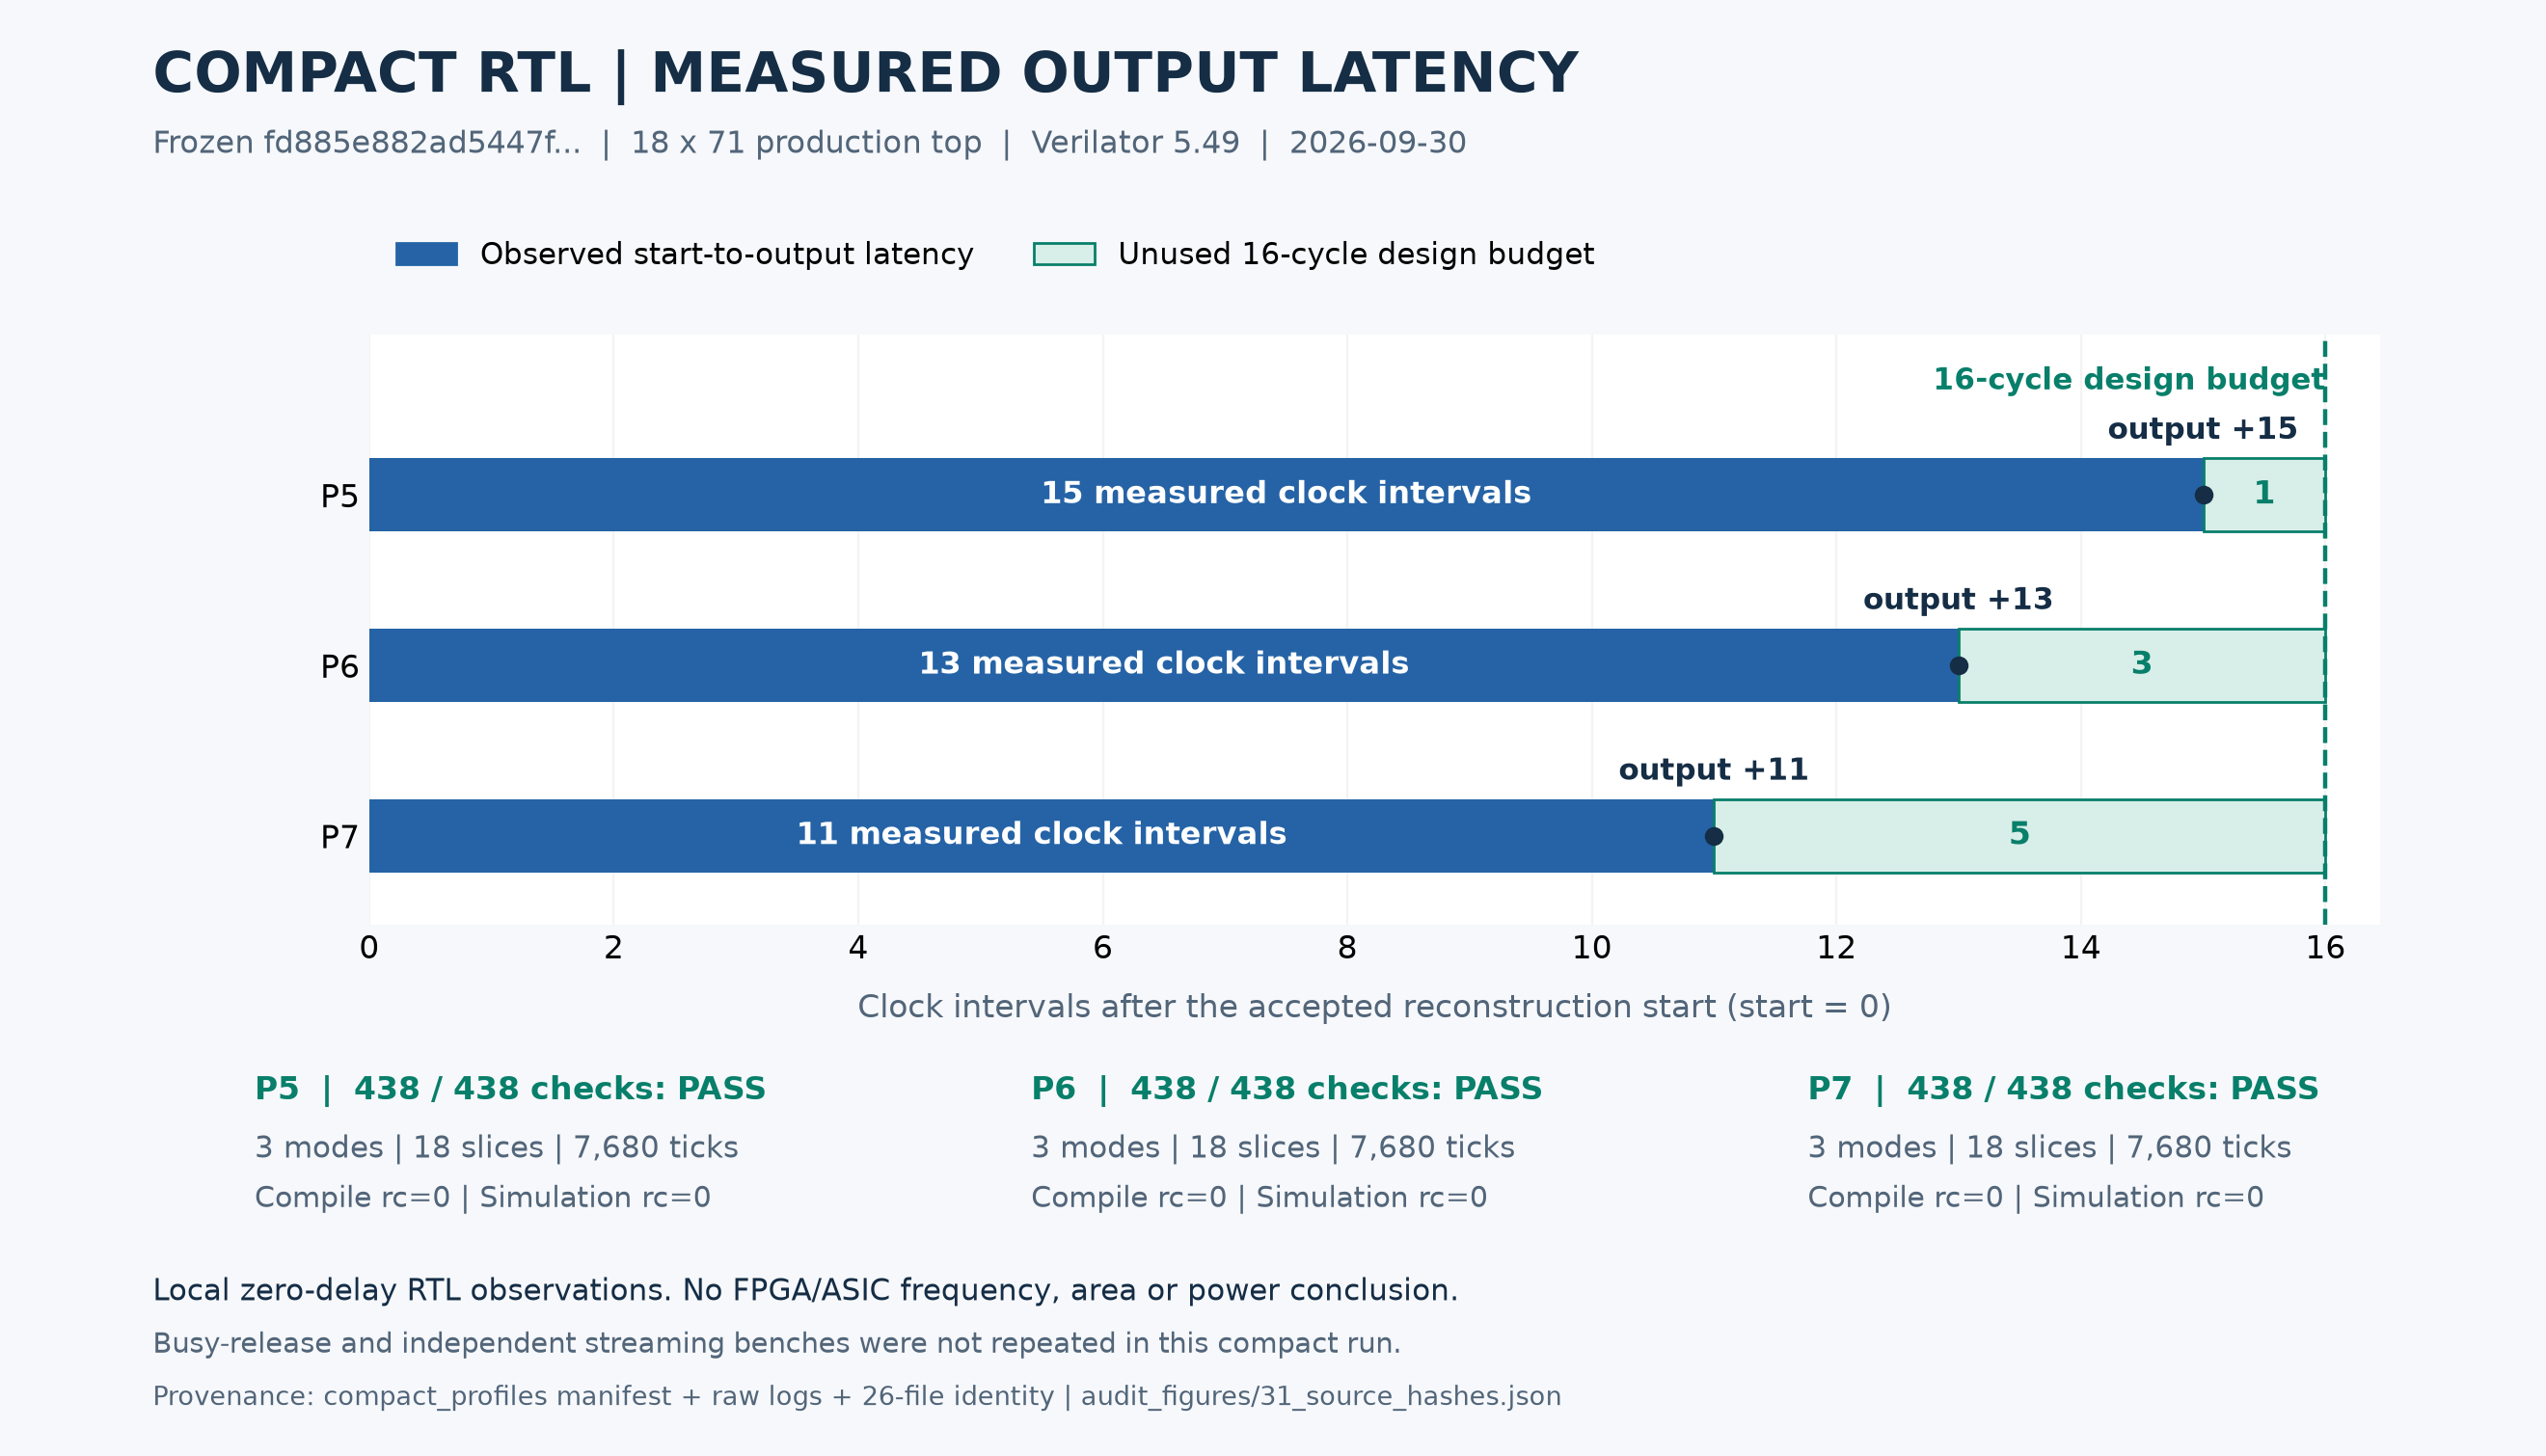
\includegraphics[width=\textwidth]{figures/31_divider_profiles.png}
\caption{P5/P6/P7 的数字周期预算与前代 \code{compact_profiles/} 实测输出延迟；源码内容摘要为 \code{fd885e882ad5}。横轴是数字时钟拍数，没有门级时延，不能据此推导640\,MHz达标。}
\end{figure}

\section{Vivado 可执行筛选与实跑条件}
新增 \code{synth/run_vivado_ssh.py} 和 \code{run_vivado_ooc.tcl}，显式指定已安装FPGA器件，统一顶层、OOC模式、1.5625\,ns周期、0.05\,ns不确定度、零I/O延迟；比较5/6/7展开配置，保留源文件与全部头文件SHA、工具版本、参数、分层资源、关键路径、DRC及vectorless功耗报告。零I/O延迟仅是筛选假设，真实宏接口预算须后续补齐。完成工件、参数及无驱动门禁检查后，runner归一化结果码0才表示受约束setup WNS非负；Windows外层raw 0本身不能作为这一判据。该状态也不表示hold、未约束端点、DRC或布线签核通过。

旧默认地址直连失败后，按用户给出的参考会话核对SSH配置，已通过 \code{windows-codex} 登录Windows主机，实测启动Vivado 2018.3，并确认 \code{xc7vx690tffg1761-2} 已安装。本轮请求1.5625\,ns，工具实际舍入为1.563\,ns；两线程、顺序运行以限制资源占用。最初两份仅替换reducer的快照均因无驱动缺陷被否定；新的完整对照共同修复树连接，再比较归约与除法组合优化。51项mock/Tcl流程测试验证打包、参数、状态校验、Windows编码与失败传播，不能替代实跑结果。实际综合、映射功能与实现结果的口径见第\ref{ch:synthesis-repair}章；ASIC PPA仍需标准单元库与物理实现结果。

\section{2026-09-30 复核修订与解释边界}
本次独立复核重算原证据清单的63项SHA-256，全部一致；同时核实基线PR的9项CI已全部成功。哈希核对确认交付文件与清单一致，不单独证明每项科学结论。复核发现报告中证据归属和文献映射的错误，已纠正如下：P3测试台计数不再被当成DUT ID；具体学习算法不再被归为论文已披露；百万码oracle写明小尺寸恒等构造；63+8分段注明工程选择；[10]补上基于dither修改粗码的必要路径，[14]将claim 1与claim 12分开；[12] tracking区分专利覆盖差距和论文强制结构；补列论文两端口dither范围扩展尚未闭合。

算术说明也需与实现一致：\(r=x-2^k\lfloor x/2^k\rfloor\) 是非负余数；96-bit合法区间包含 \(-2^{95}\)，只在小于该下界时溢出。采样dither后的\emph{合成}轨系数 \(s=1-2on+r\) 可以为 \(-2,0,2\)，有别于单独轨 \(r=\pm1\)；有符号表示至少需3bit。单笔 \code{result_flags} 与历史粘滞输出必须分列，历史异常不会因后一正常结果自动消失。

本次新增定向验证及 RTL 变更的状态、命令、源文件摘要与结果见仓库审查记录：\par\noindent\code{docs/rtl/FULL_AUDIT_20260930.md}。\par{}原始16项CI仅对其基线成立；旧版修复基线的21项本地全量回归与三参数结构回归分别登记于 \code{final_rtl/}、\code{final_profiles/}；前代定向复验与compact三参数另立清单。当前缓存提交的22项RTL CI和9项workflow结论各有独立归档，不能追溯伪装成旧CI结果。模拟宏与目标ASIC库映射、PVT及布线后签核是独立验收项；本轮FPGA实验按第\ref{ch:synthesis-repair}章的限定口径解释。
\chapter{精确除法器：位宽证明、结构改进与时序边界}
\label{chap:divider-timing}

\section{问题为何集中在除法器}
数字重构需要的是精确整数码，不能容忍依据信号正负或除法余数偶发相差一个码。
\code{recon_core} 送入除法器的分子是经 96-bit 溢出检查后右移 33 位的有符号 63-bit 数，
分母是完整的无符号 64-bit 权重和。保留该分母的高位具有明确的异常与边界语义，
不能因为正常配置的权重较小就直接截断。下述修改只涉及恢复余数法的实现，
不改变输入快照、配置 epoch、结果 ID、异常保持策略、默认 7 级展开或 16 相位入口。

2026 年 9 月 30 日的初次 Vivado 2018.3 诊断在 Virtex-7
\code{7vx690t-ffg1761-2} 上报告：\code{u_recon/u_div/mag_reg[62]}
到 \code{u_recon/u_div/q_reg[60]} 的 setup 路径延迟为
17.389\,ns，含 135 级逻辑及 119 个 CARRY4；1.563\,ns 周期下 slack 为
$-15.874$\,ns。其中逻辑延迟 12.810\,ns，估算布线延迟 4.579\,ns。
\textbf{同批完整顶层网表另有归约树被常量化问题，因此这些数字只用于定位真实存在的除法链，
不能作为有效的全设计 PPA 对照基线。}路径中标明 \code{unplaced}，也不能称为布线后 STA。
有效网表的重新综合与实现结果须独立引用对应源码冻结清单。

原实现每拍连续消耗 7 个分子位；一位的余数决定下一位是否减去分母。
因此 7 级在数据依赖上串行，\(\lceil63/7\rceil=9\) 拍的运算次数
不意味着每一级拥有 9 个时钟周期。给这条逐拍更新的路径加 multicycle 或 false-path
会改变约束含义，不能解决电路问题。本轮没有增加这类例外约束。

\begin{figure}[H]\centering
\begin{tikzpicture}[box/.style={draw,rounded corners,minimum height=9mm,align=center,fill=blue!5},arr/.style={-{Latex[length=1.8mm]}}]
\node[box,minimum width=19mm] (r) at (0,0) {余数寄存器\\$R_0$};
\node[box,minimum width=21mm] (s1) at (2.6,0) {移入一位\\试减、选余数};
\node[box,minimum width=21mm] (s2) at (5.4,0) {移入一位\\试减、选余数};
\node (dots) at (7.5,0) {$\cdots$};
\node[box,minimum width=21mm] (s7) at (9.6,0) {第 7 级\\试减、选余数};
\node[box,minimum width=19mm] (rn) at (12.3,0) {余数寄存器\\$R_7$};
\draw[arr](r)--(s1);\draw[arr](s1)--(s2);\draw[arr](s2)--(dots);\draw[arr](dots)--(s7);\draw[arr](s7)--(rn);
\node[align=center] at (6.1,-1.15) {同一时钟间隔中的 7 级真实依赖；修改后仍保留这一迭代结构};
\end{tikzpicture}
\caption{恢复余数法的一拍展开。图示解释源码数据依赖，不是仿真波形或综合测量。}
\end{figure}

\section{把比较与减法合为一次借位运算}
设当前试探余数为 $X$，寄存分母为 $D$，两者均为 $W$ 位无符号数。
原代码分别描述 \code{X >= D} 和 \code{X - D}，由综合器决定是否共享逻辑。
新代码显式用一个 $W+1$ 位结果：
\begin{align}
\Delta&=\{0,X\}-\{0,D\}\pmod{2^{W+1}},\\
q_i&=\neg \Delta_W,\qquad
R_{i+1}=q_i\,\Delta_{W-1:0}+(1-q_i)X.
\end{align}
因为 $-(2^W-1)\le X-D\le2^W-1$，最高位为 1 当且仅当发生借位，
故它同时给出比较结果；低 $W$ 位直接作为成功试减后的余数。
对于高位分母旁路，下述 \code{dv_large} 还会强制 $q_i=0$。

\begin{table}[H]\centering\small
\begin{tabularx}{\textwidth}{p{36mm}XX}\toprule
生产配置中的对象&修改前&修改后\\\midrule
分子／分母接口&63-bit 有符号／64-bit 无符号&保持全部输入位的数值语义\\
余数寄存器&65 bit&63 bit\\
分母寄存状态&64 bit&63-bit 低位与 1-bit 高位分类\\
每一级源码运算&65-bit 比较、条件减法&64-bit 扩展试减，借位作选择\\
每拍展开／迭代拍数&7 级／9 拍&7 级／9 拍\\
重构输出延迟&11 个完整时钟间隔&11 个完整时钟间隔\\
\bottomrule\end{tabularx}
\caption{可由源码确认的变化。寄存位数与运算表达式不是映射面积、功耗或频率测量。}
\end{table}

这一改写确保比较与差值来自相同的试减运算，但不能按“少写一个比较”估计 LUT 数减少一半。
旧综合器可能已经部分共享两条表达式，末级符号恢复、余数选择器和布线也会影响关键路径。
119 个 CARRY4 的诊断结果说明宽进位链串行是实质问题；本次收窄和表达式合并是低风险改进，
并不足以在未经新综合的情况下推断 640\,MHz 已达到。

\section{为何 63-bit 余数足够，64-bit 分母仍然精确}
令 $A=|a|$，$P_k$ 为按从高位到低位次序已经消耗的分子前缀。
对于 $d>0$，恢复余数法保持
\begin{equation}
P_k=Q_kd+R_k,\qquad 0\le R_k<d,\qquad R_k\le P_k\le A.
\end{equation}
下一步移入 $b\in\{0,1\}$ 时，试探余数
\(X=2R_k+b\le2P_k+b=P_{k+1}\le A\)。
有符号 $W_A$ 位输入满足 $A\le2^{W_A-1}$，包括最小负数，
所以 \textbf{余数与移位后的试探值都可用无符号 $W_A$ 位表示}。
展开需要的高位补零只增加前导零前缀，不改变该不变量。
因此生产配置取 $W=63$ 足够，无需沿用 $\max(W_A,W_D)+1=65$。

当 $W_D>W_A$ 时，对完整分母计算
\begin{equation}
L=\bigvee d[W_D-1:W_A].
\end{equation}
$L=1$ 意味着 $d\ge2^{W_A}>A$，因此幅度商必为零，内部幅度余数为 $A$。
新电路把该分类结果与分母低位同拍保存为 \code{dv_large} 和 \code{dv}；
所有试减商位强制为零，最后仍对负数执行精确 floor 修正。
这里省掉的是已能由不等式判定的宽比较，\textbf{没有丢弃分母高位的信息}。
$L=0$ 时分母低 $W_A$ 位就是完整分母，借位运算直接适用。
$W_D\le W_A$ 的参数实例将 $L$ 固定为零，窄分母作无符号扩展。

设恢复除法输出幅度商 $Q$ 和幅度余数 $R$，则
\begin{equation}
\operatorname{floor}(a/d)=
\begin{cases}
 Q,&a\ge0,\\
 -(Q+\mathbf{1}_{R\ne0}),&a<0.
\end{cases}
\end{equation}
内部 $R=|a|\bmod d$ 与负数 floor 定义中的 $a-qd$ 并不是同一个余数；
前者仅用于判定是否整除。例如 $a=-8,d=3$ 时内部 $Q=2,R=2$，
最终商为 $-3$，而 $a-qd=1$。
对最小负数 $a=-2^{62},d=1$，幅度 $2^{62}$ 能用 63 位无符号数保存，
最终负商恰好仍在 63 位有符号域中；不能先在同位宽有符号域求一个正的绝对值。

\section{固定延迟、异常与独立验证}
除法器空闲接受 \code{start} 的沿记为 $t$。接受沿只保存输入并置 \code{busy}；
随后 9 个迭代沿消费全部 63 位，在 $t+9$ 输出商、\code{err} 与单拍 \code{done}。
忙期间的 \code{start} 被忽略，输入变化不替换已保存分母的高位分类；
\code{q/err} 在下一次完成以前保持。
重构在其接受沿先保存输入，下一沿启动除法，除法完成后的下一沿提交码与元数据，
因而总延迟仍为 11 拍，能保留每 16 拍一次的输入节拍。
\code{cfg_ready} 撤销导致重构取消并复位除法器，此协议由集成控制负责。

$d=0$ 仍按固定延迟完成并返回 $q=0,err=1$；零分母判定直接检查完整输入，
并不把截断后的低分母为零误认作除零。
\code{recon_core} 将除零与本样本增益错误合并，输出阶段发出有效事件、保留前一次合法码，
并随本样本 ID 提交结果标志。粘滞错误位与 \code{result_flags} 是两个不同对象：
前者保留历史异常，后者说明当前样本。除法器的结构改写没有改变这些接口。

\begin{table}[H]\centering\small
\begin{tabularx}{\textwidth}{p{43mm}Xr}\toprule
独立检查&覆盖和完成门禁&通过数\\\midrule
Python 任意精度 oracle&有符号 63-bit 分子、完整 64-bit 分母；最值、$2^k\pm1$、多种分母位长；9 拍延迟&10,048\\
约简位宽全穷举&$W_A=6,W_D=8$；展开级数 1、2、3、7，各穷举全部输入&65,536\\
窄分母／最小位宽&$6/5$ 位、展开 5；$2/1$ 位、展开 1&2,056\\
相邻算术模块回归&MAC 任意精度比较；ADC2 舍入与完整输入域随机；输出 flags 时序&40,010／40,000／8 组\\
\bottomrule\end{tabularx}
\caption{本次修改后的独立检查。小位宽合计 67,592 组，每例同时验证定义不等式、除零、延迟、busy 和结果保持。}
\end{table}

约简位宽测试直接核对 $qd\le a<(q+1)d$（$d>0$），并检查接受后的忙状态、
未完成时旧结果保持、忙期间拒绝新请求、完成沿忙状态清除以及 \code{done} 单拍脉冲。
生产位宽 oracle 由固定种子 20260930 生成，使用 Python 整数 \code{//}，
不导入项目原有浮点模型。长商输入与超大分母分别覆盖，避免全 64 位均匀随机分母
导致绝大部分答案仅为 0 或 $-1$ 的盲区。进程正常退出、唯一完成标记和精确计数共同构成通过条件。

\begin{table}[H]\centering\small
\begin{tabularx}{\textwidth}{>{\raggedright\arraybackslash}p{40mm}>{\raggedright\arraybackslash}X}\toprule
仅在临时副本注入的错误&实际 oracle 检出结果\\\midrule
移除高分母保护&第 7 例：$a=-2^{62},d=2^{63}$，错误商 0，正确商 $-1$；进程失败。\\
移除负数余数补偿&第 4 例：$a=-2^{62},d=3$，错误商 $-1537228672809129301$，正确商 $-1537228672809129302$；进程失败。\\
\bottomrule\end{tabularx}
\caption{负对照证明 oracle 能识别本次改写最关键的两类错误。生产 RTL 未注入缺陷。}
\end{table}

\begingroup\raggedright
紧凑原始证据位于仓库 \code{docs/evidence/20260930/divider/}：
\code{arithmetic.manifest.json} 记录完整位宽检查及源码 SHA；
\code{exhaustive.manifest.json} 与 \code{exhaustive.run.log} 记录六组参数穷举；
\code{mutations.json} 及对应失败日志记录负对照。
本轮 \code{div_floor.sv} 的 SHA-256 为
\code{cc3b0bd9c5e6c8491af10d0696f82e59373426c538c3212c210093dbc84c515c}。
这些结果证明所列输入集和协议判据成立；完整生产位宽并未穷举，也不是形式化等价证明。\par\endgroup

\section{ASIC 640 MHz 的后续可实施路径}
验收边界是 ASIC 640\,MHz 目标与 FPGA 可实现频率验证。FPGA 的 LUT、CARRY4 和布线结构
不能直接换算成目标 ASIC 单元库的面积或时序；同样，FPGA 可工作并不代表 ASIC 已完成 STA。
本轮先保留已验证、修改集中的借位优化，由有效全顶层网表识别新关键路径。
如果除法仍主导，存在严格保持最终输出语义的缩域方法：
\begin{equation}
\begin{split}
a<0&\Rightarrow C=0,\quad clip_{low}=1;\\
a\ge0,\ (a\gg20)\ge d&\Rightarrow C=2^{20}-1,\quad clip_{high}=1;\\
\text{其余}&\Rightarrow 0\le q<2^{20},\quad R_0=a\gg20.
\end{split}
\end{equation}
上述分类以 $d>0$ 为前提；除零与 MAC 异常仍保留原样本错误协议。
在第三类只须从 $R_0$ 开始处理 $a[19:0]$ 的 20 个商位，所有分子位和余数仍被精确保留。
这是针对最终饱和输出的等价变换，不能直接替换一个对外承诺完整 63-bit 商的通用除法接口。

若目标库仍要求切断 64-bit 进位传播，可把借位链切成四段，每段约 16 bit，并交织样本上下文。
一条每拍接收一次试减的 radix-2 流水，每样本需要 20 次试减，平均需求为
$20/16>1$，所以单条资源不可能维持 II=16；两条共享流水各接收每隔 32 拍的样本才有足够服务能力。
另一个候选是每轮产生两位的 radix-4：并行试减 $d,2d,3d$，每样本 10 轮，
但需额外处理 $3d$ 生成、余数选择、流水上下文及元数据延迟。
这两条方案均会增加寄存状态和控制成本，应比较映射后的面积、最长路径和翻转活动，
不能仅按减法器个数宣布 PPA 优势。
若实施更深流水，必须同时变更结果 ID/flags 的上下文队列、清配置取消行为、固定输出延迟和拥塞证明，
并重新运行独立 oracle、集成吞吐与取消回归。本轮未用这种复杂架构替换已验证的默认实现。


\chapter{综合语义修复与实际 FPGA 实验}
\label{ch:synthesis-repair}
本章区分三类实验：用于定位错误的失效网表、通过独立功能见证的小单元网表，以及完整顶层的综合和实现。它们采用的 DUT 尺寸、通过判据和可推论范围不同，不能合并成一个笼统的“Vivado PASS”。所有原始失败工件保留；最终评审状态通过额外记录说明，不覆盖历史 manifest。

\section{为什么原先的综合数字必须作废}
第一次完整顶层综合虽然生成了利用率和时序报告，日志却出现五条无驱动诊断，
编号均为\code{Synth 8-3848}。
其中包括 \code{sadc_enc} 的树根计数，以及 \code{cal_weight_reduce} 的根归约量。
旧写法把节点信号定义在每个 generate 作用域中，再以
\code{g_node[2*t].total} 等前向层级名称连接子节点。
在本次 Vivado 2018.3 实跑中，这些根节点的驱动关系未被正确保留。
同一源码在 Verilator 中能正确求值，说明只用一个 RTL 仿真器不足以发现该类映射差异。

随后读取 DCP 内的网表，发现基线的 Flash 输入仅保留端口声明，没有通向逻辑的实际扇出；
归约模块则丢失了正常输入和加权树。进一步的小单元网表仿真在第一个 Flash 检查就观察到高阻态 Z，
而独立参考值为零。这是功能不一致的直接证据。
因此，原来的 35,902 LUT、65,454 FF 与 $-15.874$\,ns WNS 只保留为故障诊断数据；
同类旧列共享快照的 35,806 LUT、65,370 FF 与 $-16.228$\,ns WNS 也不属于有效 PPA 比较。
资源数很小有时意味着逻辑被错误删除，不能先把它解释为优化收益。

\section{修复的结构原则}
修复后，树边信号在模块作用域显式声明，generate 只负责给确定索引的节点赋值。
每个有效节点仍满足
\begin{equation}
Y_t=Y_{2t}+Y_{2t+1},\qquad 1\le t<L,
\end{equation}
叶子与补零规则不变，根输出仍为 \(Y_1\)。
这里 \(L\) 为覆盖有效叶子数的二次幂。
改写没有把平衡树变成一个顺序累加环，也没有增加寄存器或改变结果延迟。
所有节点有唯一驱动；padding、单叶几何和最大支持几何都必须能展开。

旧版之所以选择命名节点，是为了避免某些 lint 工具把聚合数组误判为循环。
新实现对 Verilator 使用 \code{split_var} 注释，指明常量索引元素可以分开分析；
该注释不是屏蔽 \code{UNOPTFLAT} 之类的诊断，也不会改变 Vivado 的逻辑方程。
严格 lint 继续作为失败门禁。两种工具对写法的可接受性都纳入验证后，才算解决了工程兼容性问题。

\section{同一刺激下的 RTL 与网表对照}
独立见证模块同时包含 3-bit 和 9-bit Flash 编码器，以及 3 个物理 slice、每个 2 主加 1 子单元的归约器。
它有 969 个输入位，使用 48-bit 系数、64-bit 总和和 66-bit 带符号轨和。
这是一种为快速映射检查选定的小尺寸，不是 18\(\times\)71 生产几何的替代。

参考算法逐个物理单元累加，既不遍历 DUT 的树，也不调用 DUT 的借位或归约辅助函数。
12,904 个默认检查由五组构成：128 个 3-bit 编码器输入位型、512 个 9-bit 温度计状态、
3072 个合法两-slice 选择与开关/模式组合、8192 个全部地址编码与轨模式组合，
以及 1000 个全 48-bit 系数和非温度计 Flash 位型的伪随机组合。
相同 testbench 分别驱动原始 RTL 和 Vivado 导出的功能网表。

\begin{table}[H]\centering\small
\begin{tabularx}{\textwidth}{p{36mm}X X X}\toprule
版本&RTL 语义检查&网表输入因果&XSim 功能检查\\\midrule
旧前向引用写法&12,904 次通过&959/969 个输入无端点扇出&首个 Flash 检查失败，得到 Z\\
旧公式，仅修树连线&12,904 次通过&969/969 个输入有端点扇出&12,904 次通过\\
列共享公式，修树连线&12,904 次通过&969/969 个输入有端点扇出&12,904 次通过\\
\bottomrule\end{tabularx}
\caption{相同独立见证下的真实对照。扇出恢复是必要条件；逐值检查进一步检验函数，二者不能互相替代。}
\end{table}

小单元映射的旧公式连接修复版为 2834 LUT，列共享修复版为 1837 LUT，两者均为纯组合见证，
FF 和 DSP 为零。该实验说明列共享在这个具体尺寸和工具设置中有资源收益，
但不能把减少的 997 LUT 或局部比例外推到包含系数存储、MAC、调度和除法器的完整 ADC 数字顶层。
错误旧版只剩 2 LUT，明确排除在收益计算之外。

\IfFileExists{figures/38_tree_mapping_trace.png}{
\begin{figure}[H]\centering
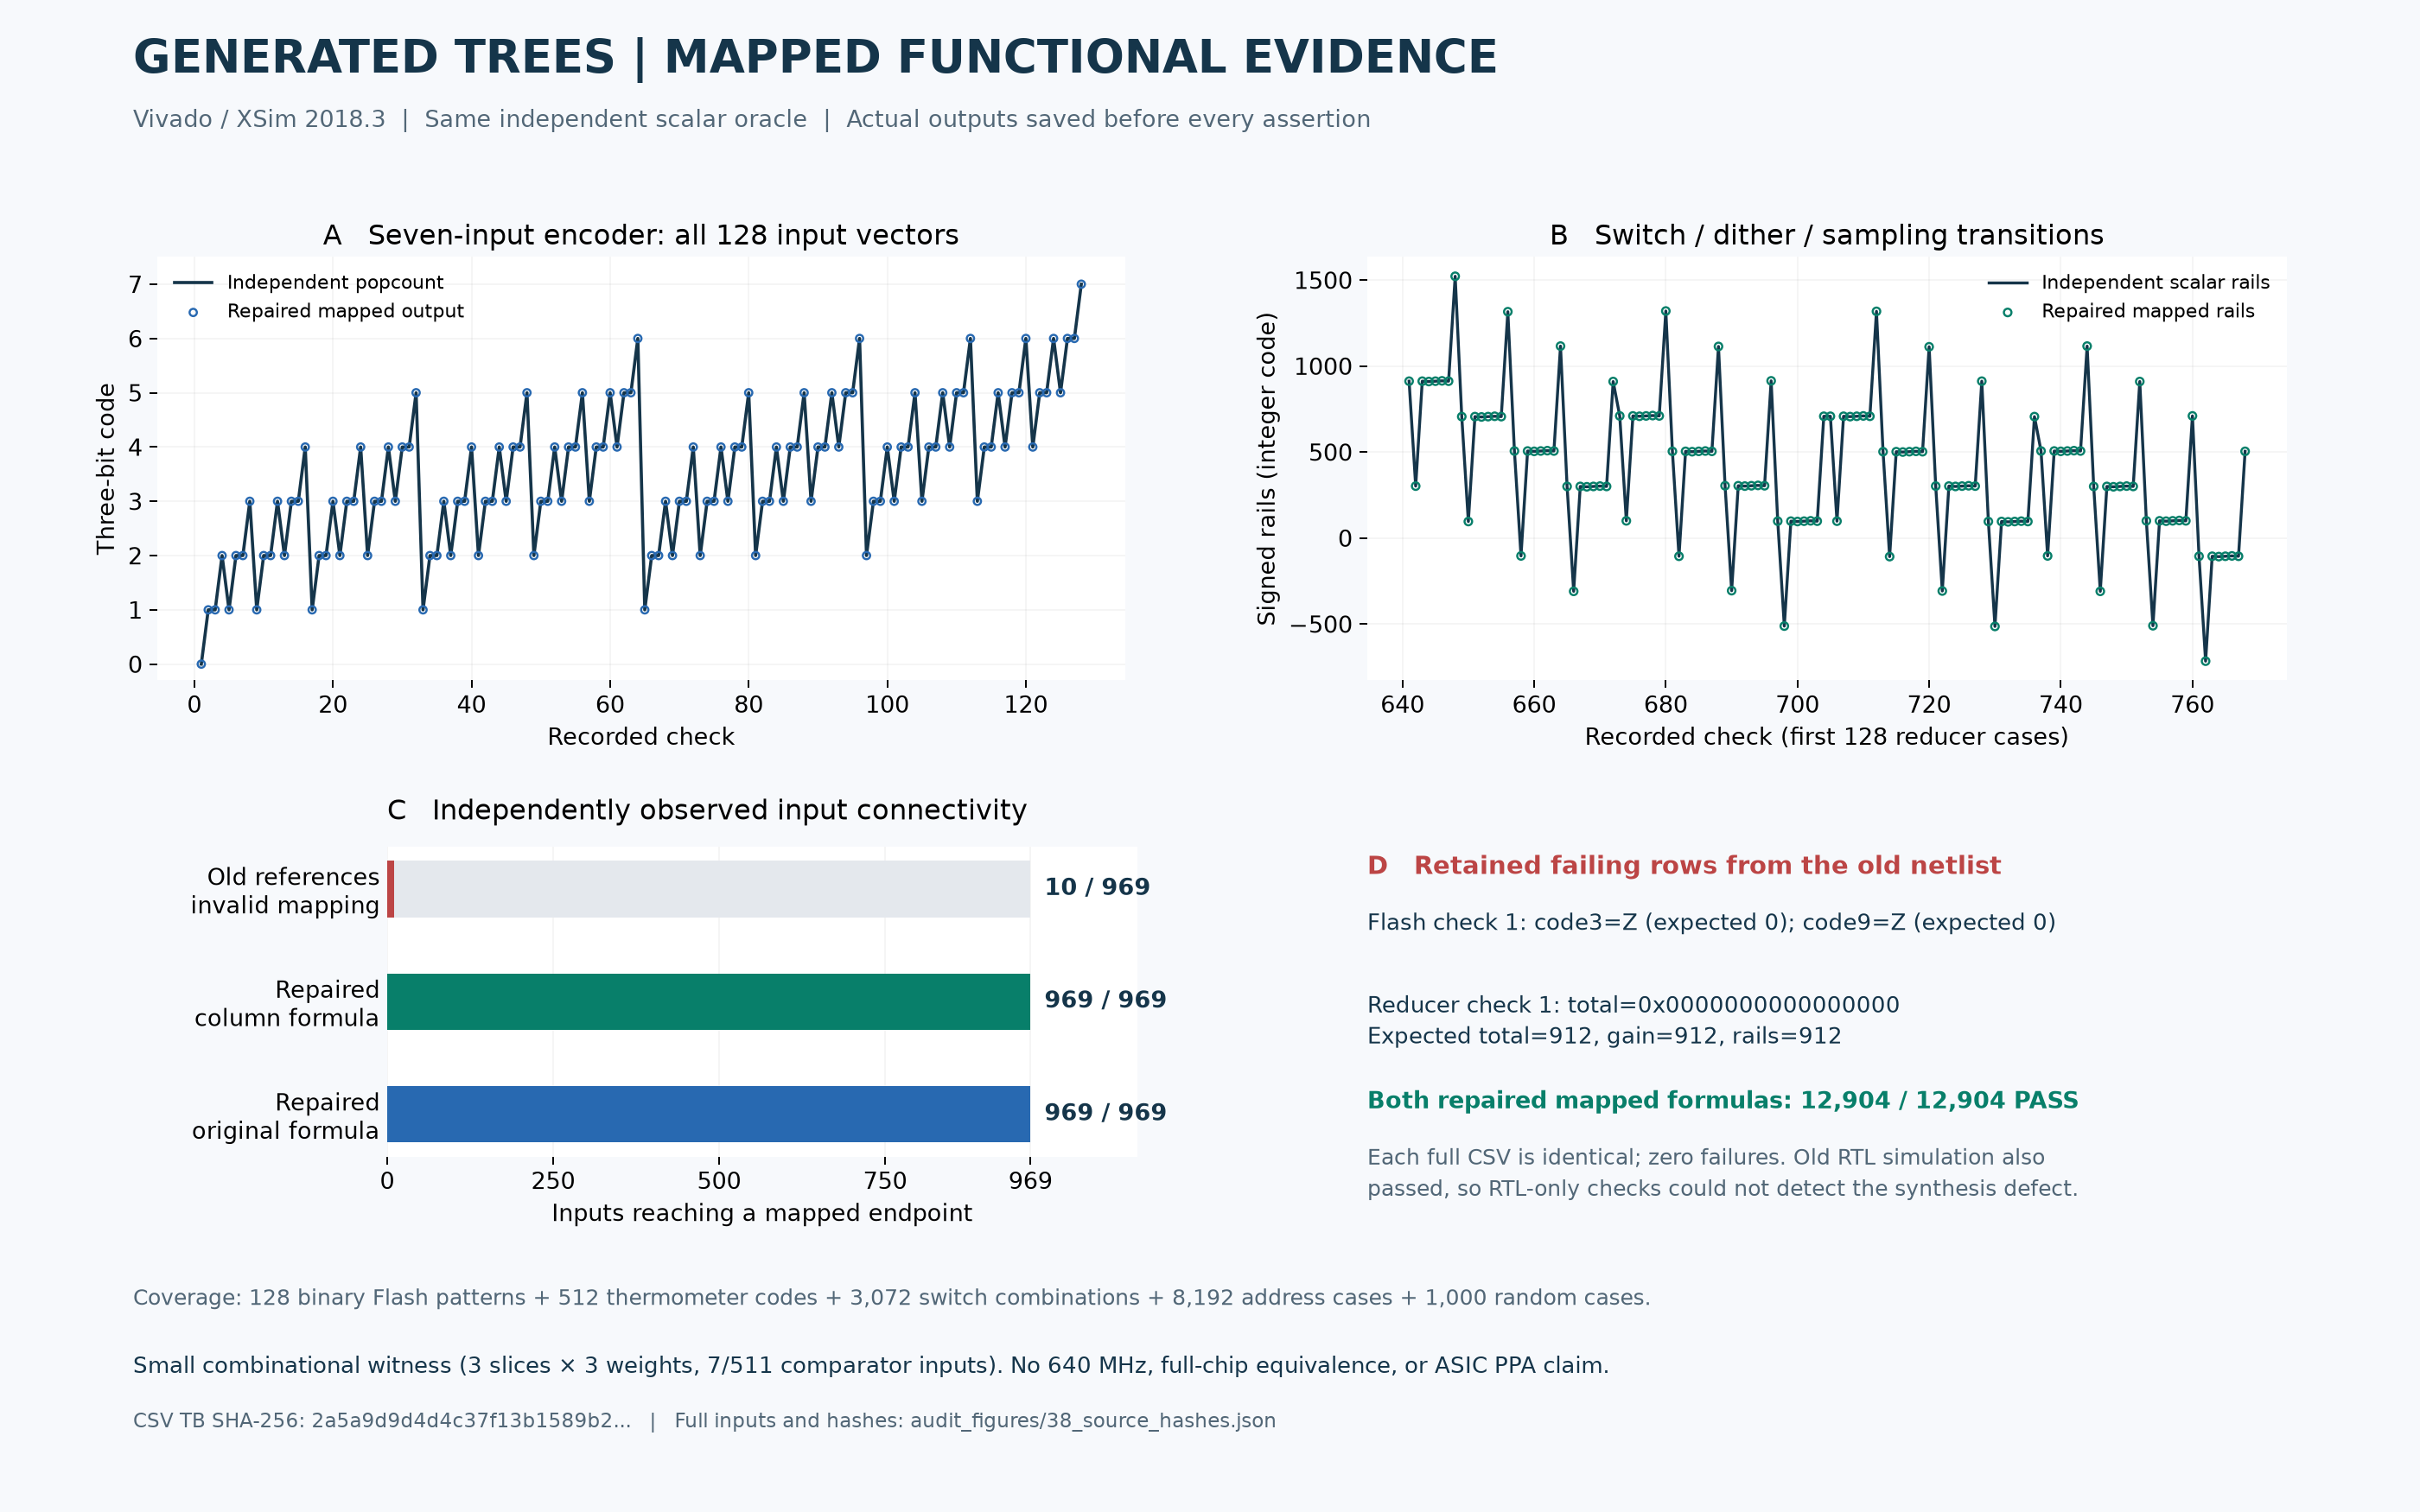
\includegraphics[width=\textwidth]{figures/38_tree_mapping_trace.png}
\caption{映射见证的实际输出、期望值和故障行。图由原始 XSim CSV 及输入扇出记录生成；高阻/未知值作为错误保留，不转换为数值零。}
\end{figure}
}{}

\section{完整顶层的公平对比条件}
新完整基线和优化版均先修复树连线与 Flash 编码器的映射问题。
基线保留列共享之前的归约公式和原除法实现；优化版包含列共享与借位复用两项算术优化。
因此，完整顶层前后差异属于这两项优化的组合效果；若要分别归因，还需要增加仅改变其中一项的实验。
两份隔离快照保留所有文件 SHA，其他生产 RTL、器件、工具和脚本保持一致。
后续精简 P5 配置还包含权重恒零最高位的显式掩蔽。
因此，P7 基线对 P7 列共享/借位版是第一组公平 A/B；
该 P7 版对精简 P5 版则同时改变除法展开参数、权重存储表达式和周期约束（P5为25\,ns），
属于整体配置比较，不能把全部差值单独归因于 P5 参数，也不能称为同约束面积对照。

器件为 \code{xc7vx690tffg1761-2}，Vivado 版本为 2018.3，综合顶层为
\code{sar20_digital_core}，结构模式开启，保留全部可写物理权重。
采用 \code{out_of_context} 与 \code{flatten_hierarchy=rebuilt}，线程数为 2。
申请周期 1.5625\,ns 在该版本的时间网格上成为 1.563\,ns；报告同时保留申请值与实际值。
0.05\,ns 用户时钟不确定性和零 I/O delay 是结构筛选条件，不能据此假定真实比较器或板级接口无需建立时间。

P5/P6/P7 的 RTL 协议回归都保持 16 拍输入间隔，输出延迟分别为 15/13/11 拍。
综合配置的比较还需考虑关键路径是否从除法转移到权重归约或 MAC。
将一条路径缩短后，新的最坏路径可能来自另一模块；这是优先级转移，而不是测量矛盾。
不应只摘取 \code{u_div} 的改善值来宣称顶层频率提高。

\IfFileExists{sections/vivado_measured_table.tex}{\subsection{P7 公平 A/B 的实际结果：面积退化而非收益}
\begin{table}[H]\centering\small
\begin{tabular}{lrrr}\toprule
指标&修复后基线 P7&列共享/借位 P7&变化\\\midrule
Slice LUT&171,246&199,039&+27,793（+16.23\%）\\
FF&66,817&66,778&$-39$\\
DSP48&20&20&0\\
BRAM / latch&0 / 0&0 / 0&0\\
Setup WNS（ns）&$-17.426$&$-17.112$&+0.314\\
Hold WHS（ns）&$-0.264$&$-0.264$&0\\
Pulse width slack（ns）&+0.025&+0.025&0\\
最坏数据路径（ns）&18.941&18.627&$-0.314$\\
最坏路径逻辑级数&135&148&+13\\
该路径 CARRY4 数&117&125&+8\\
Vectorless 估计（W）&1.58&1.58&报告精度内相同\\\bottomrule
\end{tabular}
\caption{相同器件、Vivado 2018.3、P7 与申请周期1.5625\,ns的完整综合结果。均为综合后估计，尚未布局布线；功耗未使用实测开关活动。}
\end{table}

这组结果否定了“源码加法表达式变少就必然节省 FPGA 面积”的假设。
列共享与借位改写的组合使 LUT 增加16.23\%，setup只改善0.314\,ns，仍大幅违反目标。
最坏路径仍位于除法器：基线从\code{dv_reg[0]}到\code{q_reg[60]}，
改写版从\code{rem_reg[0]}到同一目标寄存器。
改写后125个CARRY4串联，说明每拍展开7步的串行借位依赖仍是主要频率障碍；
FF仅减少39个，不足以抵消组合资源增长。
因此，这一版本只能称为功能等价的算术结构候选，不能宣传已经获得低面积PPA优势。

两份\code{check_timing}的16类问题计数均为0，未约束路径表为空；
这说明记录约束下的检查覆盖，并不消除实际负setup/hold裕量。
OOC时钟尚未通过真实内部BUFG布线，且I/O延迟为零，
所以不能从18.627\,ns的综合估计直接宣布53.7\,MHz为可用频率。
后续P5以25\,ns进行FPGA筛选，另外改变了展开数、权重最高位表达式和时钟约束；
必须单列其结果。行和缓存若进入候选，也须与该P5在相同25\,ns条件下比较。

基线DCP为69,108,593字节，摘要\code{9c3bc09dd193d0bf}\ldots；
列共享/借位DCP为71,421,073字节，摘要\code{4712577f4291fed3}\ldots。
两份均已逐字节核对远端与本地SHA-256；原始报告、源归档和完整摘要见
\code{docs/evidence/20260930/vivado_complete_p7/}。
第一份运行曾在报告下载阶段超时，原失败manifest保留，随后从同一次已完成运行恢复并验证；
不能把文件传输故障混写为综合失败，也不能只凭恢复状态略去原始过程。
}{}
\IfFileExists{figures/32_vivado_comparison.png}{
\begin{figure}[H]\centering
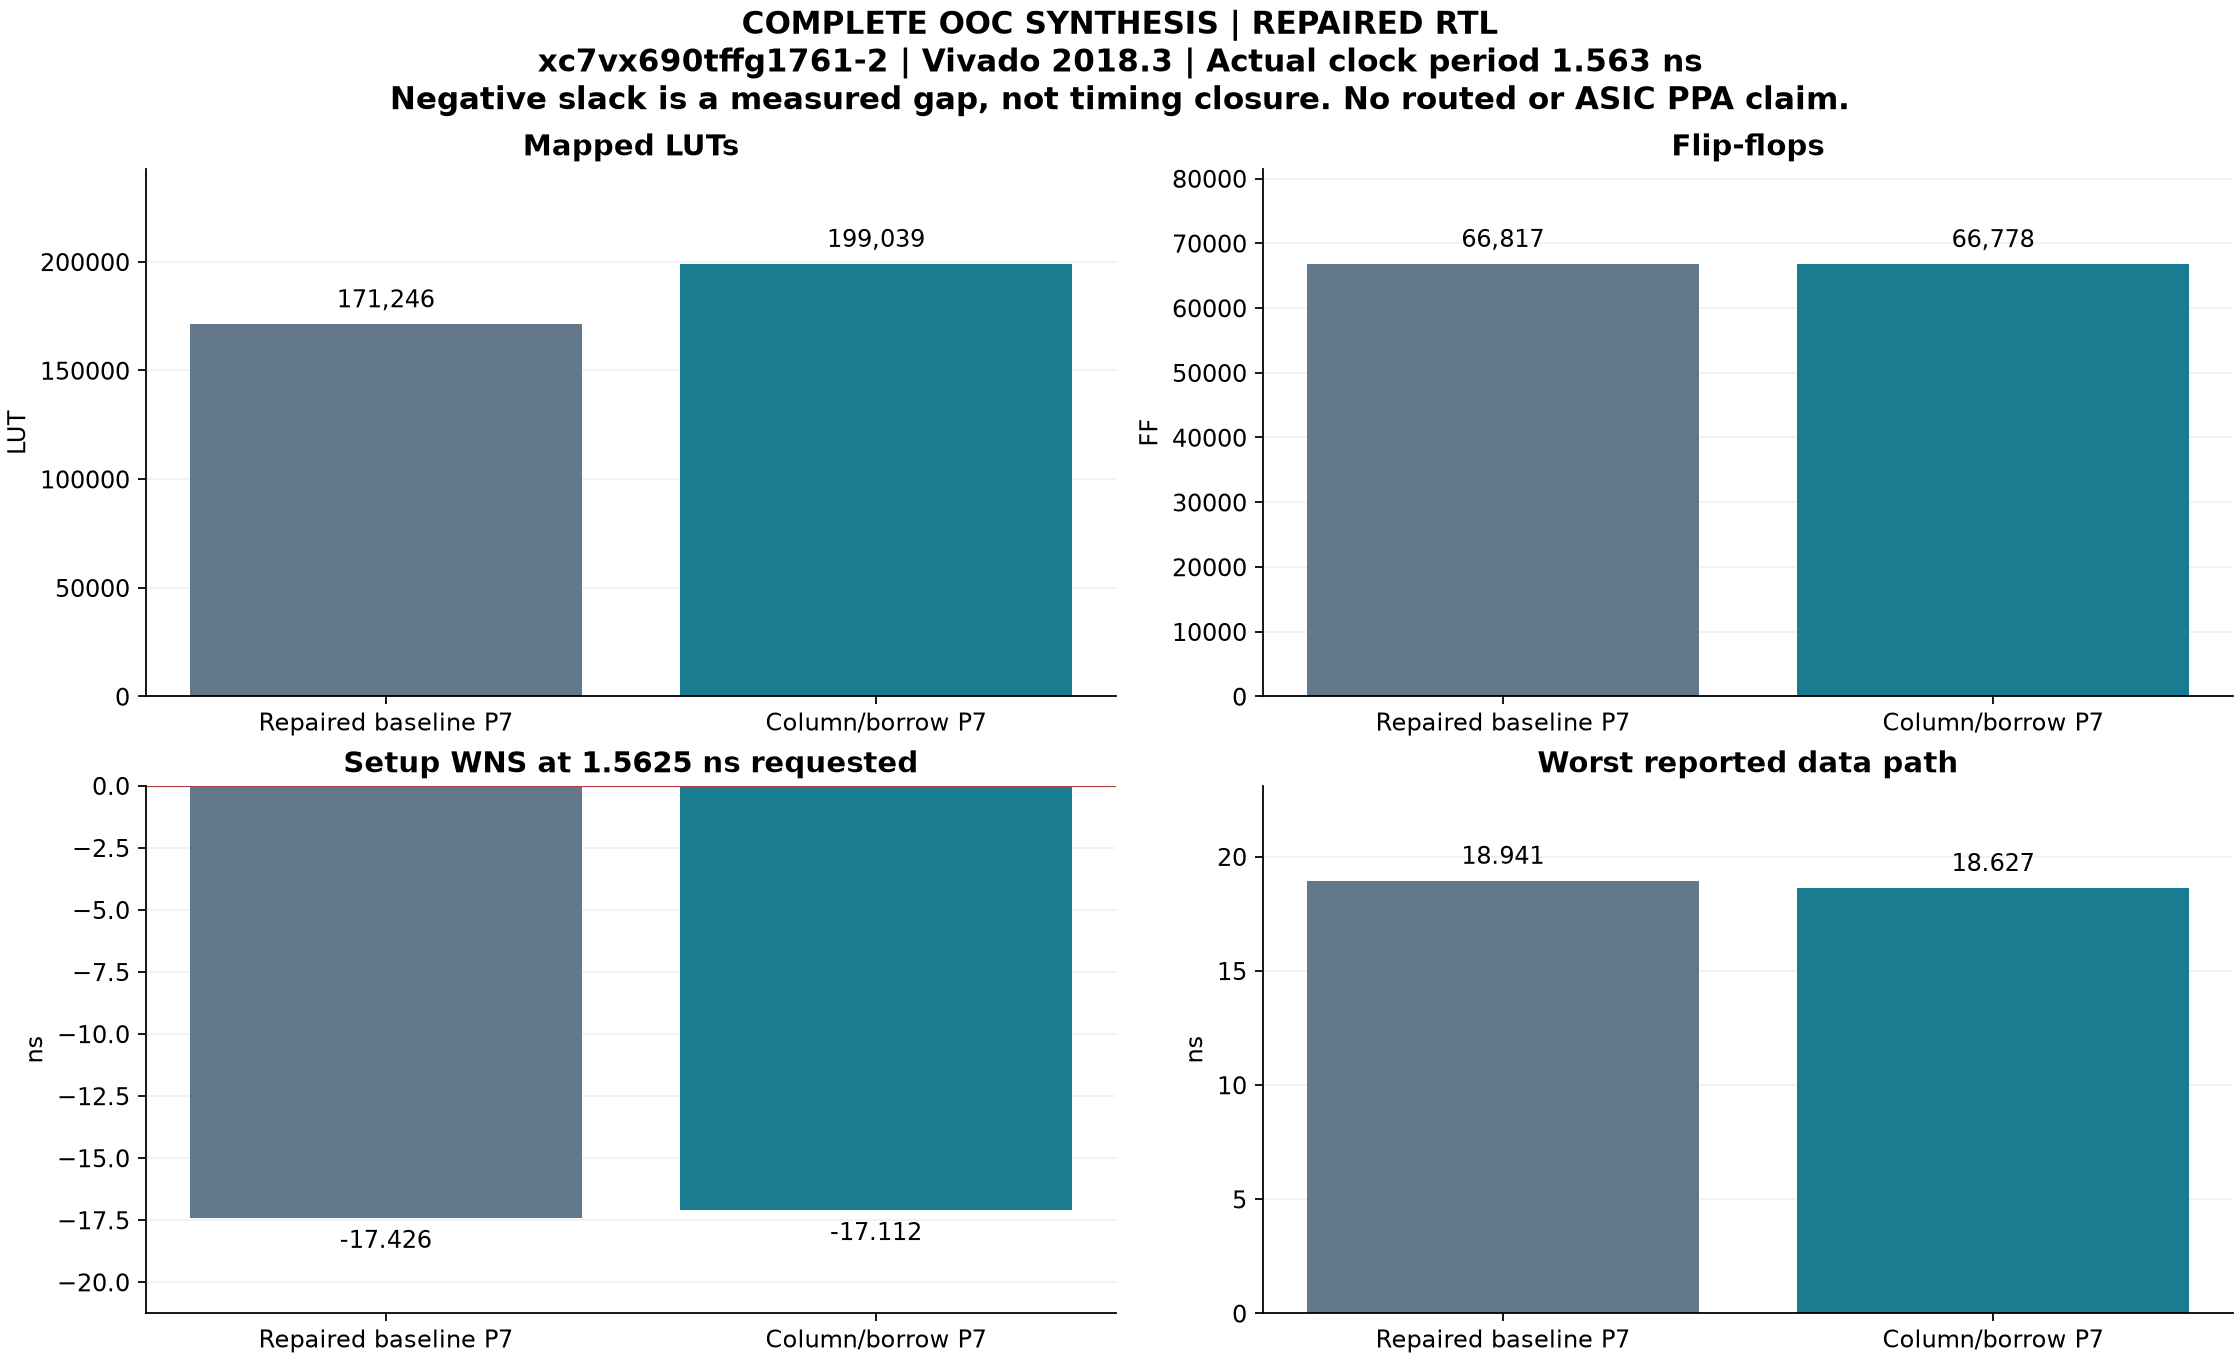
\includegraphics[width=\textwidth]{figures/32_vivado_comparison.png}
\caption{有效完整顶层快照在相同 FPGA、工具和申请周期下的综合后对照。负 WNS 表示与该目标的差距；该图不表示布线后或 ASIC 时序闭合。}
\end{figure}
}{}


\section{资源开销的解释与进一步缩减条件}
有效完整基线的 \code{weight_store} 实测为 62,622 FF，
恰好等于 \(18\times71\times(48+1)\)：每项 48-bit 系数加一位本 epoch 已写标记。
它约占该基线全部 66,817 FF 的 93.7\%。
因此，单纯把除法余数寄存器缩窄几位，无法解决主要寄存器开销。
这个数字也说明，当前“全部物理权重可同时读取”的接口具有实在的面积成本。
必须把这种成本与论文未披露的实际系数存储结构区分开。

这里还能提取一个可综合的不变量。合法写入必须满足 \(0<W<2^{47}\)，
复位将权重置零，clear 只清除已写标记，拒绝写入保持原值。
因此，从复位状态开始逐拍归纳可得所有物理权重的 bit 47 恒为零。
基线 DCP 仍存在 1278 个名为 \code{w_q_reg[s][u][47]} 的 FDRE，
表明综合器没有利用跨越写入许可逻辑的这一数值关系。
本轮后续精简版将接受写入时的存储表达式显式写为
\begin{equation}
W_{\rm stored}=W_{\rm data}\mathbin{\&}(W_{\max}-1),\qquad W_{\max}=2^{47}.
\end{equation}
对任何被接受的写入，该表达式逐位等于原始数据；原 48-bit 端口和非法写入拒绝条件不变。
这属于把已经成立的常量位显式暴露给综合器，不是降低合法系数精度。
实际删除数量仍以该精简版 DCP 和资源表为准，不能仅按预计数填入测量栏。
\begin{figure}[htbp]
  \centering
  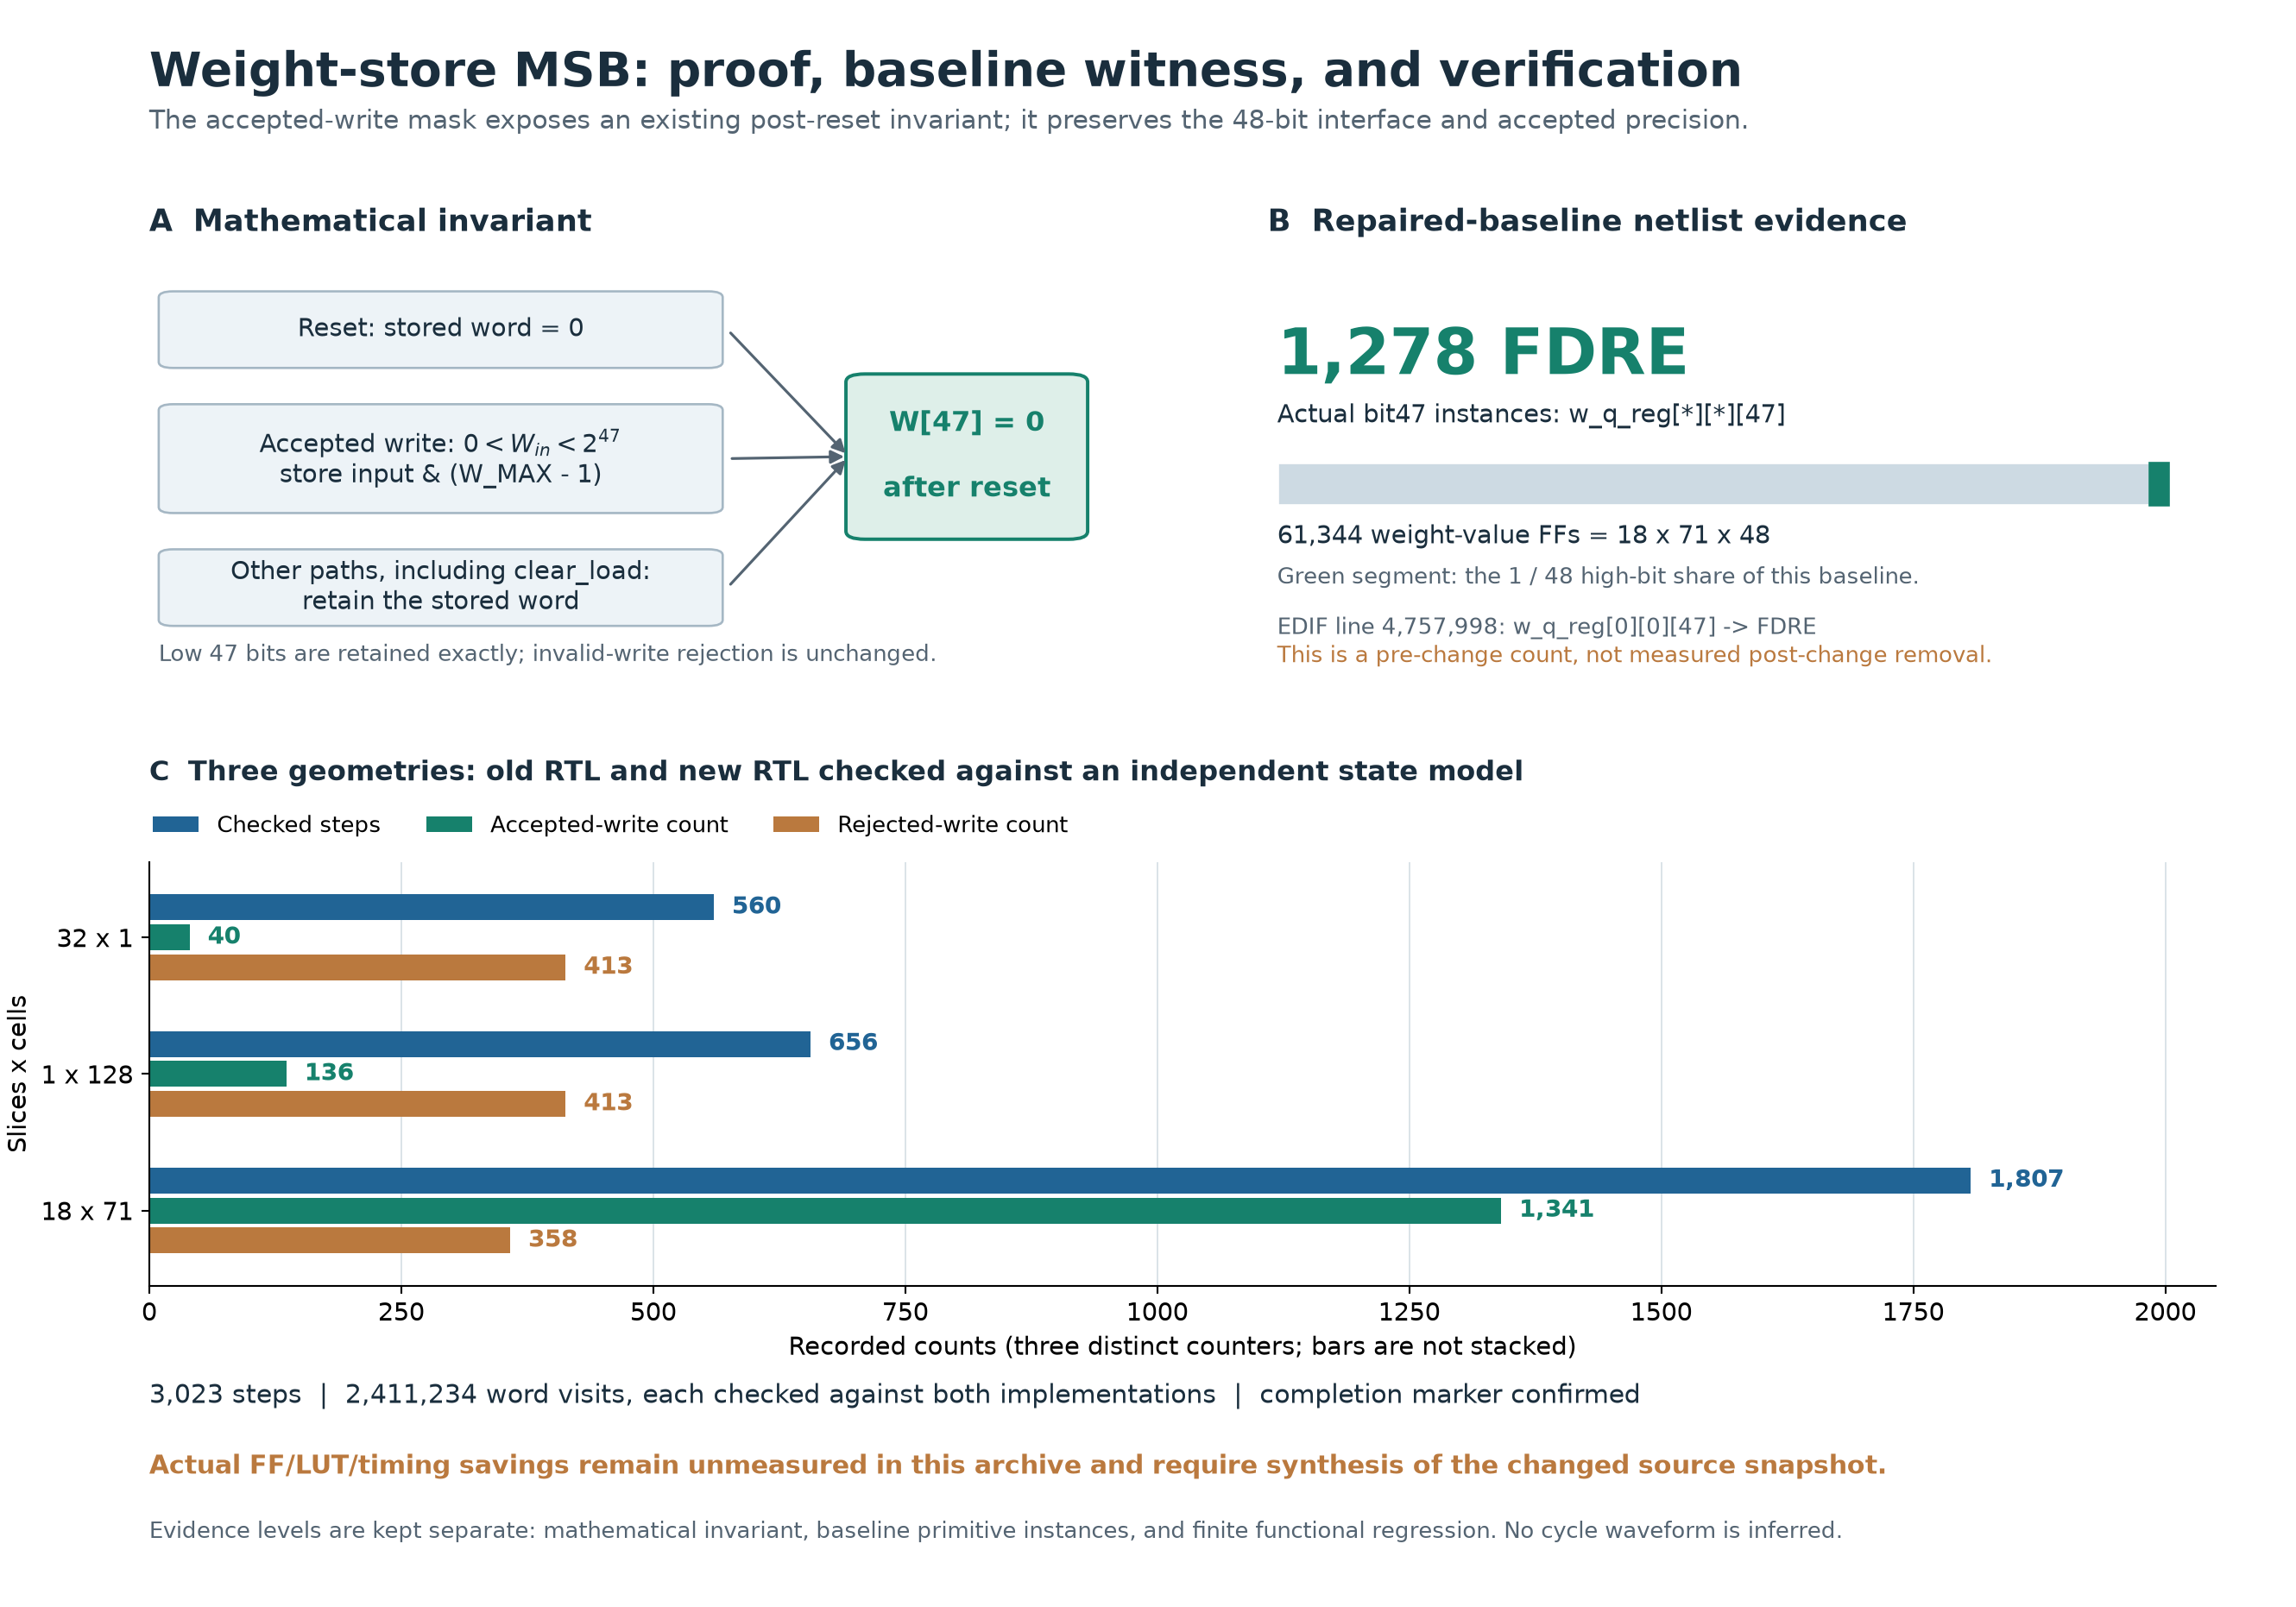
\includegraphics[width=\textwidth]{figures/40_weight_msb_evidence.png}
  \caption{权重存储最高位优化的三层证据。A：复位写零、合法写入满足$0<W<2^{47}$、其他分支保持原值，因而可由归纳法证明复位后的$W[47]=0$；显式写入掩码保留低47位及原有非法写入拒绝行为。B：修复后的基线网表中，61,344个权重数值触发器确实包含1,278个第47位FDRE实例，绿色段仅表示这一基线的$1/48$份额，不能解释为已测得的优化后面积节省。C：三种几何配置的独立状态参考分别检查560、656、1,807步，共3,023步；接受写入、拒绝写入与检查步数是三个不同计数器，图中不堆叠、不相加。按各配置的检查步数乘以存储单元数，共访问2,411,234个权重字，每次均对照修改前、修改后实现；不能再将两种实现的比较次数倍增为覆盖数量。数据来自\code{weight_msb/verification_manifest.json}、\code{equiv.run.log}与\code{vivado_structure/baseline_weight_msb_witness.json}，制图脚本逐项核对归档哈希与完成标记。图中没有重建逐拍波形；修改后真实FF、LUT和时序收益仍需对相应源码快照重新综合测量。}
  \label{fig:weight-msb-evidence}
\end{figure}


综合报告没有推断出 BRAM。若改为块 RAM，必须同时设计读端口数、系数供给带宽、
样本上下文流水与 epoch 清空协议，不能只把数组声明换一个关键字。
每笔 8 个活动 slice、每个 71 个权重，若完全逐项读取则每笔至少需要 568 次系数访问。
16 拍启动间隔意味着平均至少 35.5 项每拍；这是访存下界，尚未计入配置读回和装载。
即使总带宽足够，每个活动物理 slice 都需要在窗口内供出自身 71 项，
所以按 slice 分 bank 的双端口 RAM 还会遇到每 bank 的独立带宽限制。
增加复制读端口、预存前缀和或装载期预聚合，都需要新的面积、同步和数值等价测量。

另一个无需增加寄存器的组合候选是利用同一物理行的共享选择条件：
\begin{equation}
T=\sum_s A_s\!\left(\sum_u W_{s,u}\right),\qquad A_s\in\{0,1\}.
\end{equation}
它把逐权重选择改为逐行总和选择；开关项若能证明 \(on_{s,u}=1\Rightarrow A_s=1\)，
也可以消去重复的活动行门控。
但生产几何下，简单二级平衡树可能形成 \(7+5=12\) 层，原全局树为 11 层。
活动行控制到输出可能缩短，而系数寄存器到输出可能增长；因此必须分别测量两类路径，
不能只数门控数量便断言时序改善。这一候选尚未计入本轮资源收益。

静态 \(T\) 与部分模式相关 \(G\) 可以候选地在配置装载期累计，
但当前结果依赖物理 slice 组合、采样 dither 掩码和 DEM 后的物理开关。
对 \(R\) 的优化必须保留真实 \(on\) 与轨极性，不能把物理失配权重退化为均匀权重或名义码乘常数。
一种可检查的推进顺序是：先缓存每个 slice 的总和与专用采样单元和，
再将未加权的选择状态同缓存版本一起锁定到 epoch；
最后以现有逐物理单元 oracle 对最大系数、所有模式、重复地址及 clear 中断逐值核对。
上述方案中的每行总和缓存已在后文实现并做定向验证；专用采样单元和缓存、额外流水及存储bank仍为候选。功能验证通过不等于面积改善，行和缓存的资源收益须以独立同约束综合对照为准。

还需注意 \code{flatten_hierarchy=rebuilt} 的资源归属。
Vivado 会在扁平优化后重建层级，逻辑可以跨原始 RTL 边界移动；
例如有效基线重建的 \code{cal_sample_context} 接口包含原 RTL 没有的归约相关端口。
因此，“该层级下 LUT 很多”不能直接推成“打包上下文寄存器产生了这些 LUT”。
顶层利用率才是整体 A/B 比较的直接计数；模块优化的归因还需要保留边界的独立综合、
原始 primitive 连接与功能检查，不能只根据重建层级名称修改 RTL。

\section{可实现频率与布局布线验收}
用户确认的验收口径允许 FPGA 使用实测可实现频率，并保留 ASIC 640\,MHz 目标。
实现流程读取已验证和冻结的 DCP，不覆盖原综合结果；在新输出目录设置明确周期，
依次运行 \code{opt_design}、\code{place_design}、\code{phys_opt_design} 和 \code{route_design}。
setup、hold、脉宽、路由完整性和 DRC Error 分别检查，不能只按 setup WNS 生成成功标记。

原始外部时钟筛选流程通过 \code{HD.CLK_SRC} 指定实际存在的 BUFGCTRL site。
AMD/Xilinx 文档明确指出：当缓冲器位于 OOC 模块之外时，该全局时钟不在模块实现中实际布线；
该属性提供驱动位置/类型以改进时钟延迟、偏斜与共同路径悲观移除估计。
因此，本次进一步准备了带内部 BUFG 的实现流程：仅断开顶层 \code{clk} 端口与原时钟网的直接连接，
将端口接至 BUFG 输入，再以其输出驱动原来的完整时钟负载集合。
ECO 前后所有时钟端点的排序列表、数量与 SHA-256 必须相同；只允许增加一个 BUFG，
不能因引入时钟缓冲而删改数据通路或丢失寄存器。

实现后另检查 BUFG 输出网的实际 \code{ROUTE_STATUS=ROUTED}、非空 routing nodes/pips，
并分别读取全设计与内部寄存器路径的 setup/hold 最坏裕量。
还要求脉宽裕量非负，TNS/THS/TPWS 与三类失败端点数均为零；
\code{check_timing} 的16项覆盖计数必须齐全且全部为零，未约束与忽略路径分组必须为空。
报告缺失、字段不全、非有限数或摘要与逐路径查询不一致均不能产生通过结论。
这只说明记录下来的 OOC 约束被完整检查，不证明零 I/O 延迟适合真实板级接口。
\code{HD.CLK_SRC} 的估计上下文不再代替内部时钟布线。
该流程依然是 OOC：端口至 BUFG 输入的外部时钟边界及零 I/O delay 不是整板接口约束。
所以内部时钟实际布线与整板时钟签核必须分别表述；本流程不输出整板 bitstream 验收，
也不替代 ASIC PVT 与物理库签核。
参见 \href{https://docs.amd.com/api/khub/documents/dUZkF9u9qQ4x4MtRgpH9aQ/content}{UG905 v2018.3}。
109 个缓冲时钟流程与报告解析用例已通过；六组流程合计272项通过。
这些是前置工程验证；只有后面的实际运行表能证明布局布线结果。

Vivado runner 的 Windows 外层批处理可能在 Tcl 负时序退出后仍返回 raw 0。
流程保留原始返回码，只在完整状态文件、参数、工具版本、全部所需报告和负 WNS 一致时，
才把它解释为“综合完成、时序未满足”。任何无驱动告警则使综合完整性失败，
不能再把该网表放入有效 PPA 对照。用于控制这种行为的 mocked tests 验证流程逻辑，
真实综合/实现报告验证 EDA 的实际结果，两者分开计数。

\section{配置期行和缓存：把不随样本变化的加法移出转换路径}
\label{sec:row-cache}
P7 实测的 LUT 退化促使本轮重新选择优化对象。对于同一个生效配置 epoch，
物理系数不变，只有活跃 slice 集合与开关状态变化。因此可以把
\(H_s=\sum_u W_{s,u}\) 缓存在系数装载器中，转换时只计算
\begin{equation}
T=\sum_s A_s H_s,\qquad
G=T-M,\qquad R=T-2W_{on}+R_d.
\end{equation}
其中 \(A_s\) 是物理行是否活跃的位图，\(M\) 和 \(R_d\) 仍按实际采样轨求和。
这不是拟合算法，也不是论文披露的新电路；它是当前可编程整数校正接口的精确工程变换。
本节描述行和缓存候选。其本地22项功能回归已完成，双版本定向与负控证据见本节末；
最终PPA取舍仍须由同约束综合及实际实现结果决定。

\begin{figure}[H]\centering
\begin{tikzpicture}[node distance=8mm and 10mm,box/.style={draw,rounded corners,align=center,minimum height=12mm,fill=blue!6},arr/.style={-{Latex[length=2mm]}}]
\node[box,minimum width=37mm] (write) {接受的配置写\\地址 $(s,u)$ 与新值};
\node[box,right=of write,minimum width=44mm] (delta) {$H_s-W_{s,u}+W_{new}$\\精确替换更新};
\node[box,right=of delta,minimum width=35mm] (cache) {18 行缓存\\每行54 bit};
\node[box,below=of write,minimum width=37mm] (store) {原物理系数表\\合法值47 bit};
\node[box,below=of cache,minimum width=35mm] (sum) {活跃位图门控\\18 行归约得到 $T$};
\draw[arr](write)--(delta);\draw[arr](delta)--(cache);
\draw[arr](write)--(store);\draw[arr](store.east)-|(delta.south);
\draw[arr](cache)--(sum);
\end{tikzpicture}
\caption{候选行和缓存的工程结构示意。系数与缓存只在同一个接受写边沿更新；这是结构说明，不是仿真波形。}
\end{figure}

\subsection{逐拍不变量与 clear 的语义}
必须证明的状态关系是每个周期都满足 \(H_s=\sum_u W_{s,u}\)，
而不是仅在完整装载结束时偶然相等。复位同时令系数和行和为零。
合法接受对 \((s,u)\) 的写入时，旧值先被减去，再加新值，系数和缓存同沿提交；
其余行不变。被拒写、运行锁定和空闲周期保持二者。
\code{clear_load} 只清除本 epoch 的 written bitmap，保留系数数值，因而也必须保留行和。
clear 之后的第一次重写仍然减去保留的旧值；若把 written=0 当成“旧系数为零”，
第二个装载 epoch 就会重复累计。这是定向负控应能识别的关键故障。

活跃行由物理 ID 的 OR 位图形成。重复 ID 会报警，但数值求和仍只包含该物理行一次；
缓存实现必须保持这一原有语义，不能改为每个逻辑槽重复累加。
无效 ID 不激活任何物理行。采样 dither 的列树继续读原物理叶子，
只移除 total 树的上层加法，不能连带删除列树仍需使用的叶值。

\subsection{宽度、资源预算和配置路径的代价}
合法写入满足 \(0<W<2^{47}\)。对一行 \(U\) 个单元，
\begin{equation}
0\leq H_s < U2^{47}\leq 2^{47+\lceil\log_2 U\rceil}.
\end{equation}
生产配置 \(U=71\) 因而需要54 bit，18行共972个候选状态位。
模块支持的最大 \(U=128\) 仍满足54 bit上界；\(U=1\) 时47 bit即可。
向原64-bit归约接口补零不会改变精度。按该上界作归纳，每次减旧值无下溢，
加新值后不越出行和宽度；此证明依赖装载器的合法写守卫，不适用于任意未经检查的外部位型。

原1278个有效叶的 total 归约需要1277次非平凡加法，
18行归约需要17次，源结构减少1260次加法。
on 树和 dither 列树保留；宽系数并行读也仍存在，不能由此宣称已转换成SRAM结构。
初版新增代价包括972个状态位、被选行和的读选择、旧系数读选择、一次减法和一次加法。
初版通过装载器的 \code{selected_weight} 显式共用写替换与配置读回的旧值路径，
避免只依赖跨层级优化来合并两个宽选择器；实际布线随后揭示这条全局反馈路径过长，
因此下面另检验逐物理行局部更新候选。

配置路径仍在同一个时钟域内，每次合法写必须满足真实 setup/hold。
不能因为软件通常慢速写寄存器，就把这条路径设为 false path 或多周期。
如果最终关键路径转移到“选择旧权重—减法—加法—行和寄存器”，
应在保留当前握手语义的前提下继续处理，或者报告实际可用频率。
本候选不增加转换流水级；P5/P6/P7 的15/13/11拍与16拍启动间隔仍须实测复核。

针对首次P5实际布线时出现的全局旧系数读回路径，又冻结了仅修改
\code{weight\_store.sv}的逐物理行局部更新候选：每个slice在本地选旧系数，
对本行执行\(H_s-W_{s,u}+W_{new}\)，并仅在被接受且地址命中时提交。
它避免先汇合成一条全局旧系数再反馈到任意行，却可能复制18组减加电路；
所以不能仅凭更短的逻辑连线推断PPA收益。
此候选RTL内容摘要为\code{6b27c64df11838428e7f364ac165c5986b51be586fd8cca1722d8095e54e7a22}。
官方Verilator 5.020下22项回归与三种生产lint通过；18-slice顶层P5/P6/P7
各有三模式、438个输出、7,680个协议周期和438个延迟观测，分别为15/13/11拍。
逐项原始日志与哈希见\code{docs/evidence/20260930/local\_row\_trial\_rtl/}。
这些仅是零延迟功能结果。后述同约束综合发现其LUT增加14.66\%，
实际路由又因拥塞等级7失败，故\emph{不保留}这个逐行独立读选的版本；
图中的功能通过不能抵消物理不可布通。

\begin{figure}[H]\centering
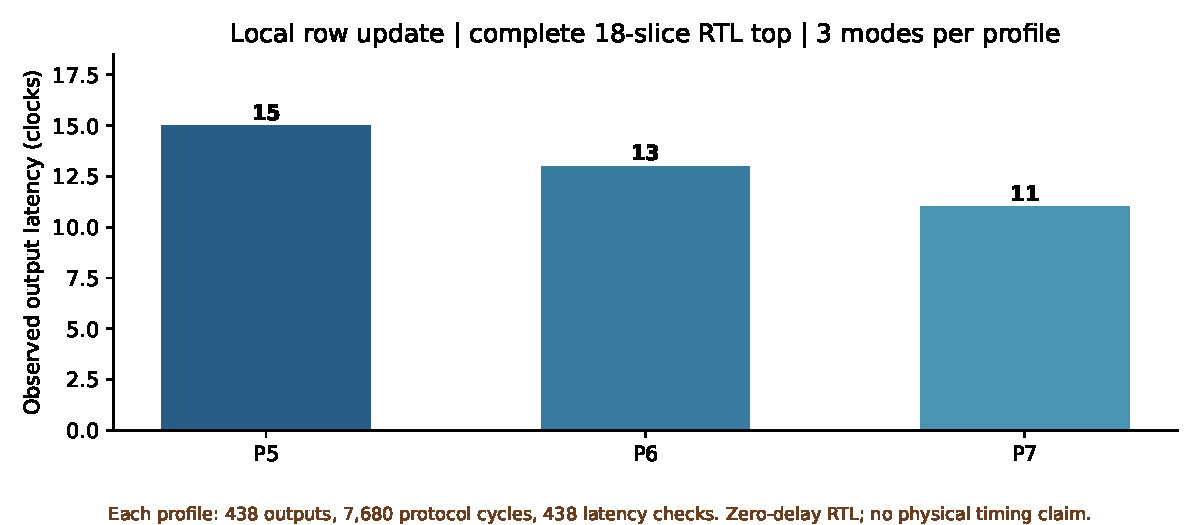
\includegraphics[width=0.84\textwidth]{figures/local_row_profiles.pdf}
\caption{局部行更新候选的实际RTL完整顶层输出延迟。三档结构的输出、周期和延迟检查数均从冻结日志重绘；脚本在作图前核对57项证据文件哈希，见\code{audit_figures/make_local_row_profiles.py}与同名\code{*.sha256.json}。柱高是数字时钟拍数，不能读作纳秒时序。}
\label{fig:local-row-profiles}
\end{figure}

\subsection{如何判定候选可以进入最终版本}
功能门禁要同时覆盖新状态不变量与使用缓存的真实生产链路。
直接驱动 \code{w_rom} 的叶模块保留常量参数关闭缓存的接口；
生产顶层开启缓存，两条路径均有独立标量参考。
定向验证应包含完整最大值行、同址连续替换、clear后重装、拒写、
32\(\times\)128边界、重复与无效ID，以及蓄意损坏一个缓存项后的失败见证。
完整结构顶层还须覆盖18个slice、三种dither模式、配置读回及 epoch 取消。

PPA门禁必须与精简P5采用相同25\,ns约束、器件和工具。
只报源码运算符削减，或只通过缓存关闭分支的回归，都不能算这一候选成功。
即使综合资源下降，仍须实际布局布线检查 setup、hold、pulse width、约束覆盖和DRC，
并对最终完整综合网表执行功能比较。

% Candidate-only evidence; root decides the final insertion point.
\subsection{行和缓存候选的双版本数值证据}
\label{sec:row-cache-evidence}
本节对应候选 RTL 内容摘要 \code{1e3fab94b7b2}\ldots，包含 26 项生产 RTL 文件；父提交为 \code{f028ec5}。
来源为 \code{docs/evidence/20260930/row_cache/}，属于新的本地功能验收，不能移用父提交 CI 的通过结论。
归档中的 Verilator 5.020 与运行时标识为 5.49 的开发版，分别完成相同的五种加载器几何和七种归约器几何。
每个版本的 16,150 个加载事务步与 1,430,848 个归约输入样本按各自单位列示，不相加为覆盖率。
5.020 的附加复验只包括这两项，不能据此声称该工具本地重跑了全部 22 个 bench。

最大装载先把整张表写为 \(W_{\max}=2^{47}-1\)，故每个含 \(U\) 项的物理行应为 \(U W_{\max}\)。
\code{clear_load} 清除完整性位图，保留权重与行和；随后将行 0 的一个旧最大权重替换为 1，
独立期望成为 \mbox{\((U-1)W_{\max}+1\)}。图\ref{fig:row-cache-evidence}分别保留原日志的 \code{row_last} 与 \code{row0} 标签。
制图器以 Python 任意精度整数重新计算，不把超过 \(2^{53}\) 的行和先转为浮点数再判断相等。
全部十个阶段观测在两个版本原始日志中逐条匹配；归档没有单独记录 clear 当拍的数值，因而不额外绘制该时刻。

\begin{figure}[H]\centering
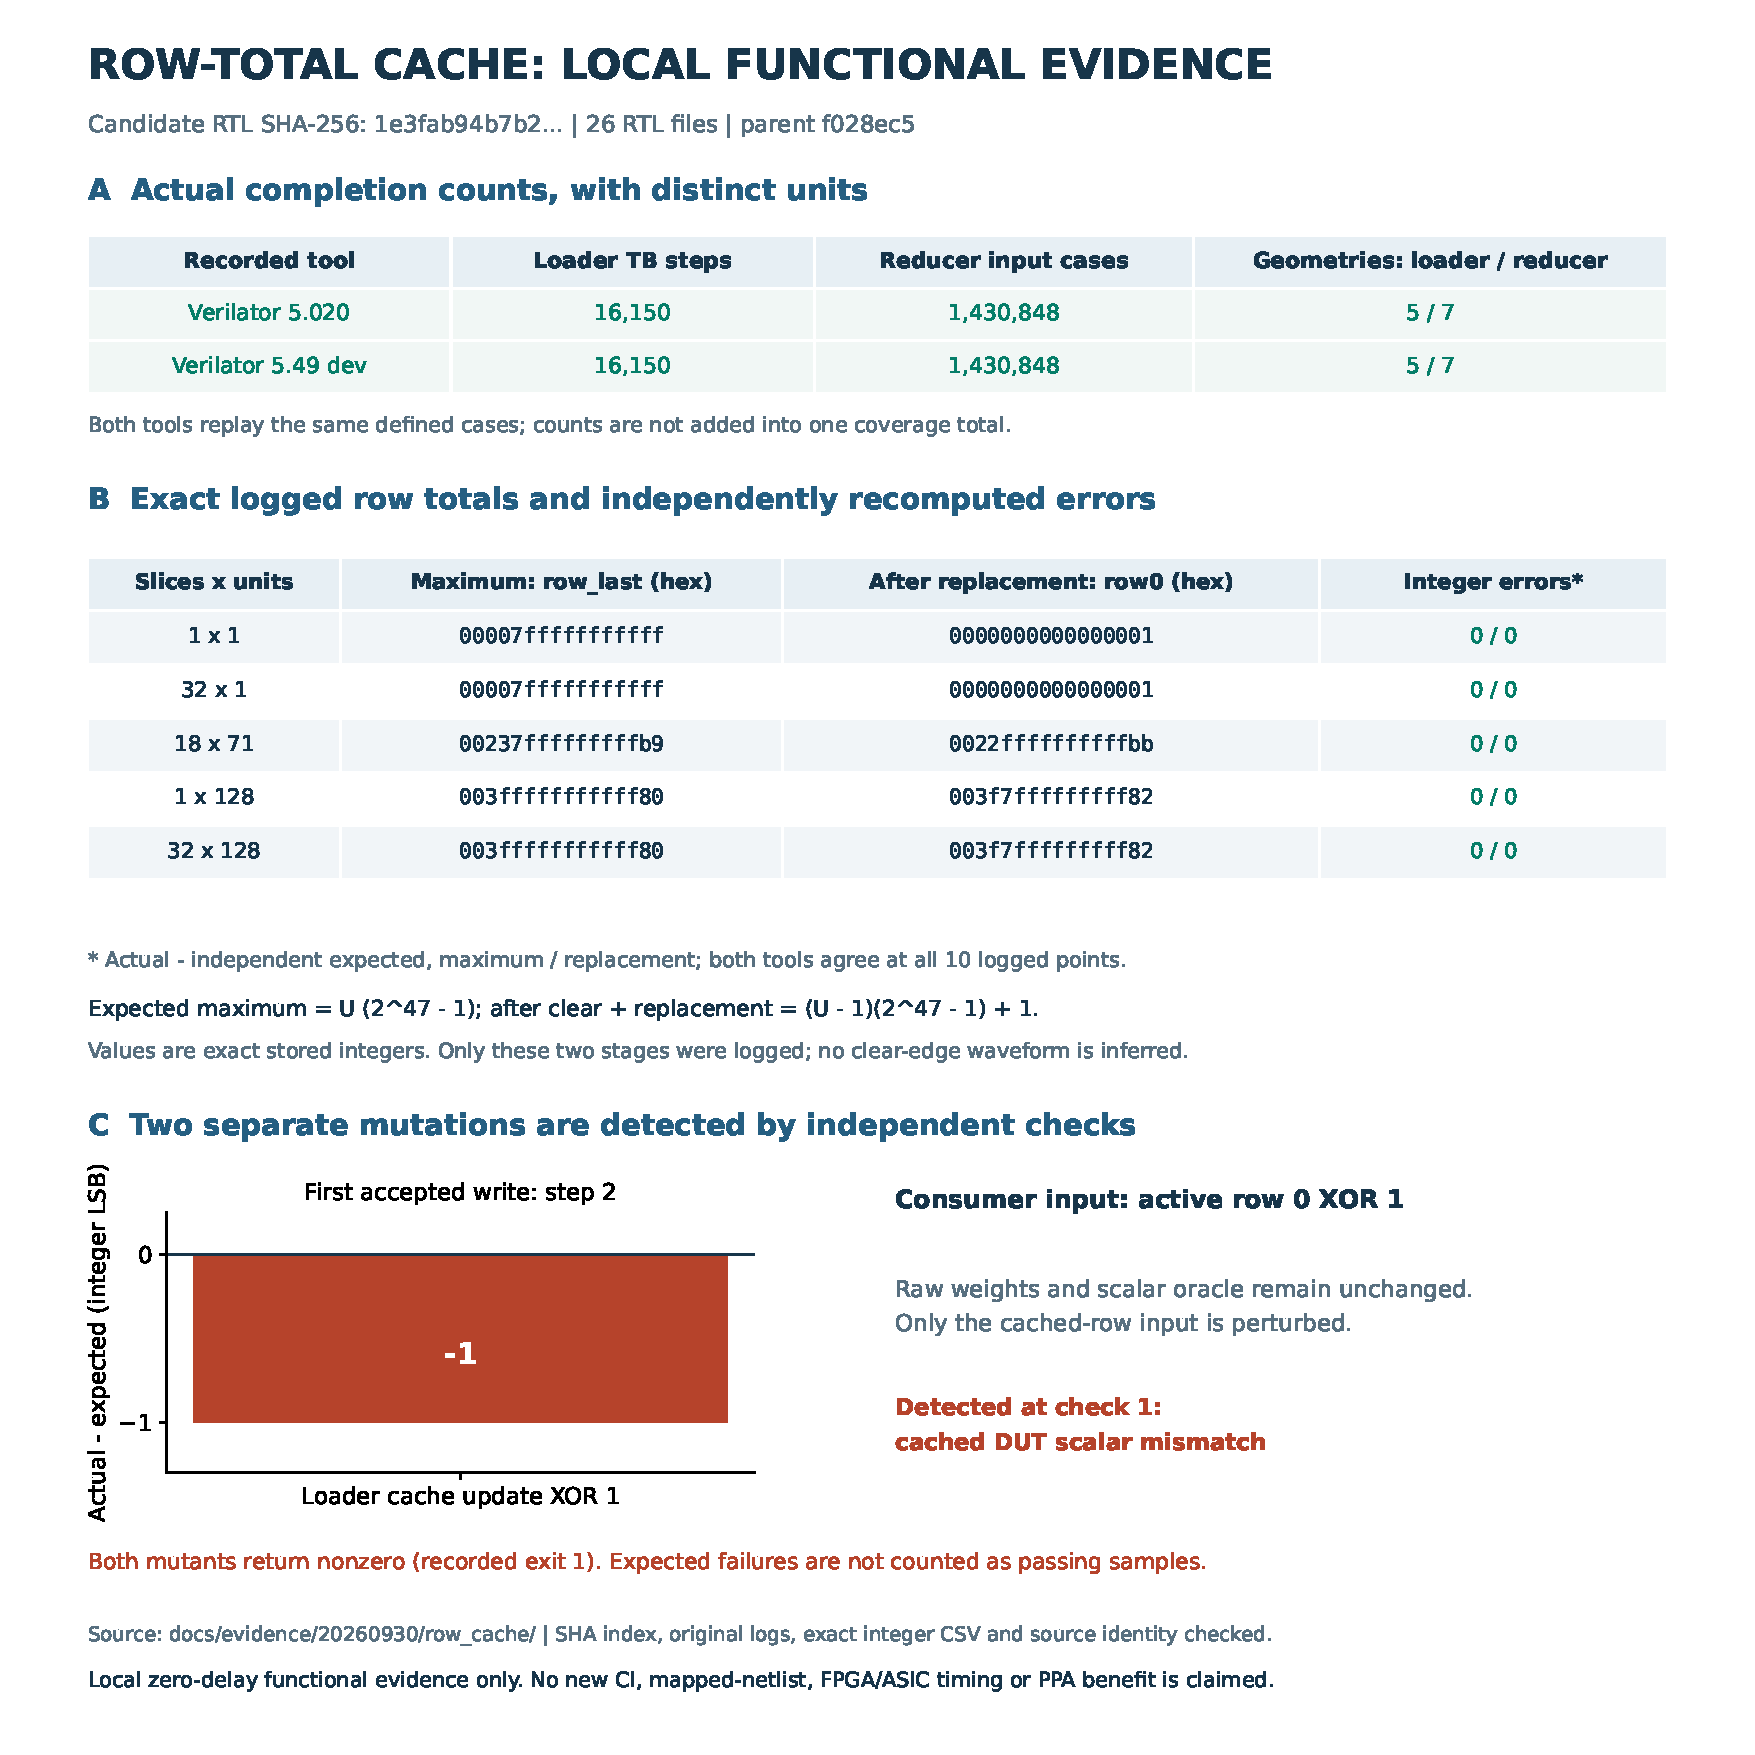
\includegraphics[width=\textwidth]{figures/41_row_cache_evidence.pdf}
\caption{候选行和缓存的真实日志证据。上表为双版本完成计数；中表为五种几何在最大装载和 clear 后替换两个已记录阶段的精确十六进制整数，独立整数公式的误差均为零。下方展示两个分别注入的错误被检出；没有由完成标记推造波形，也没有将功能通过解释为 PPA 收益。}
\label{fig:row-cache-evidence}
\end{figure}

两个负控分别检查生产者和消费者。
第一项只翻转行和写回结果的最低位，在首次接受写的第 2 步出现实际值相对独立期望少 1，加载器检查立即失败。
第二项只翻转活动行 0 的缓存输入最低位，原始权重、未缓存实现、旧公式和 scalar oracle 都不变；
第 1 个比较样本触发 \code{cached DUT scalar mismatch}。
后者排除了“缓存输入被忽略而仍通过普通数值回归”的假阳性；它不是新功能正常输出的样本。

可复现入口为 \code{audit_figures/make_row_cache_evidence.py}，来源清单为 \code{audit_figures/41_source_hashes.json}。
脚本校验归档 SHA、26 项 RTL 摘要、完成计数、十个实测值以及两份负控的失败日志与源文件摘要。
这些结果说明行和维护与消费在所测功能条件下符合独立判据；缓存候选的实际资源、物理建立/保持时序及 ASIC 目标频率仍应由同一候选的后续综合和实现报告单独判定。



\section{P5同约束对照的超时记录}
为了判断行和缓存是否真正带来面积与时序收益，已冻结前代精简版和当前缓存版的源码，
计划在相同\code{xc7vx690tffg1761-2}、Vivado 2018.3、\(P_{\rm STAGES}=5\)、25\,ns请求周期、
同一综合脚本与XDC下逐项比较。前代精简版的第一轮运行在7,200\,s运行时限处被脚本终止，
结束前仍处于时序优化阶段；没有\code{status.txt}、DCP、完整利用率或时序报告。
该轮原始失败记录见\code{docs/evidence/20260930/vivado_compact_p5_timeout/}，
其manifest摘要为\code{ad645b3f5a9304a69636b39737eb74bd0b2595060190cff0ca1b116f409501dd}。
它只说明在记录的机器负载与时限下未完成综合，不能判为WNS不达标，也不能作缓存版的PPA基线。
只有两份完整且通过无驱动检查的报告都取得后，才能填写同约束资源差值。

\subsection{当前缓存版 P5 的有效综合后快照}
当前行和缓存提交的冻结源码另在相同器件、Vivado 2018.3、P5、25\,ns申请周期下完成了一次完整 OOC 综合。
其实际远端运行\code{run.c97c940ad1274c699c40b8c78ff00602}返回\code{SYNTH_COMPLETE}；
原始\code{scp}回传在900\,s上限中断，保留失败manifest后从\emph{同一次远端运行}独立取回全部报告、
续传49,687,597字节DCP，并与远端SHA-256逐字节核对。其完整摘要由下面两行连续拼接：
\par\noindent\code{670d019aaec0efe80e060342ff0dbd74}\quad
\code{8c0029b4c01d6a42e741de32ecb05ff1}。\par
归档\code{docs/evidence/20260930/vivado_cached_p5/}的25个payload文件均通过\code{sha256.json}复验；
恢复过程没有重新综合、替换输入源码或删除传输失败记录。
原始综合日志无\code{Synth 8-3848}无驱动诊断，\code{check_timing}的16类检查全为零，
DRC无错误但有49项警告。这使下面的\emph{综合后}数值可用，但不构成布线或板级时序签核。

\begin{table}[H]\centering\small
\begin{tabular}{lrrl}\toprule
指标&实测值&器件可用值/端点总数&判读\\\midrule
Slice LUT&106,205&433,200&24.52\%\\
触发器&66,520&866,400&7.68\%\\
DSP48E1&20&3,600&0.56\%\\
BRAM tile/锁存器&0/0&1,470/866,400&未推断出BRAM\\
setup WNS/TNS&+10.640\,ns/0&200,389&失效端点0\\
hold WHS/THS&$-0.264$\,ns/$-14,943.110$\,ns&200,389&失效端点60,455\\
pulse WPWS/TPWS&+12.150\,ns/0&66,520&失效端点0\\\bottomrule
\end{tabular}
\caption{冻结的当前缓存版P5完整顶层OOC综合后报告。25\,ns是申请周期；setup通过而hold未通过，因此“全时序满足”和“40\,MHz已实现”都不是本表结论。}
\label{tab:cached-p5-synth}
\end{table}
\begin{figure}[H]\centering
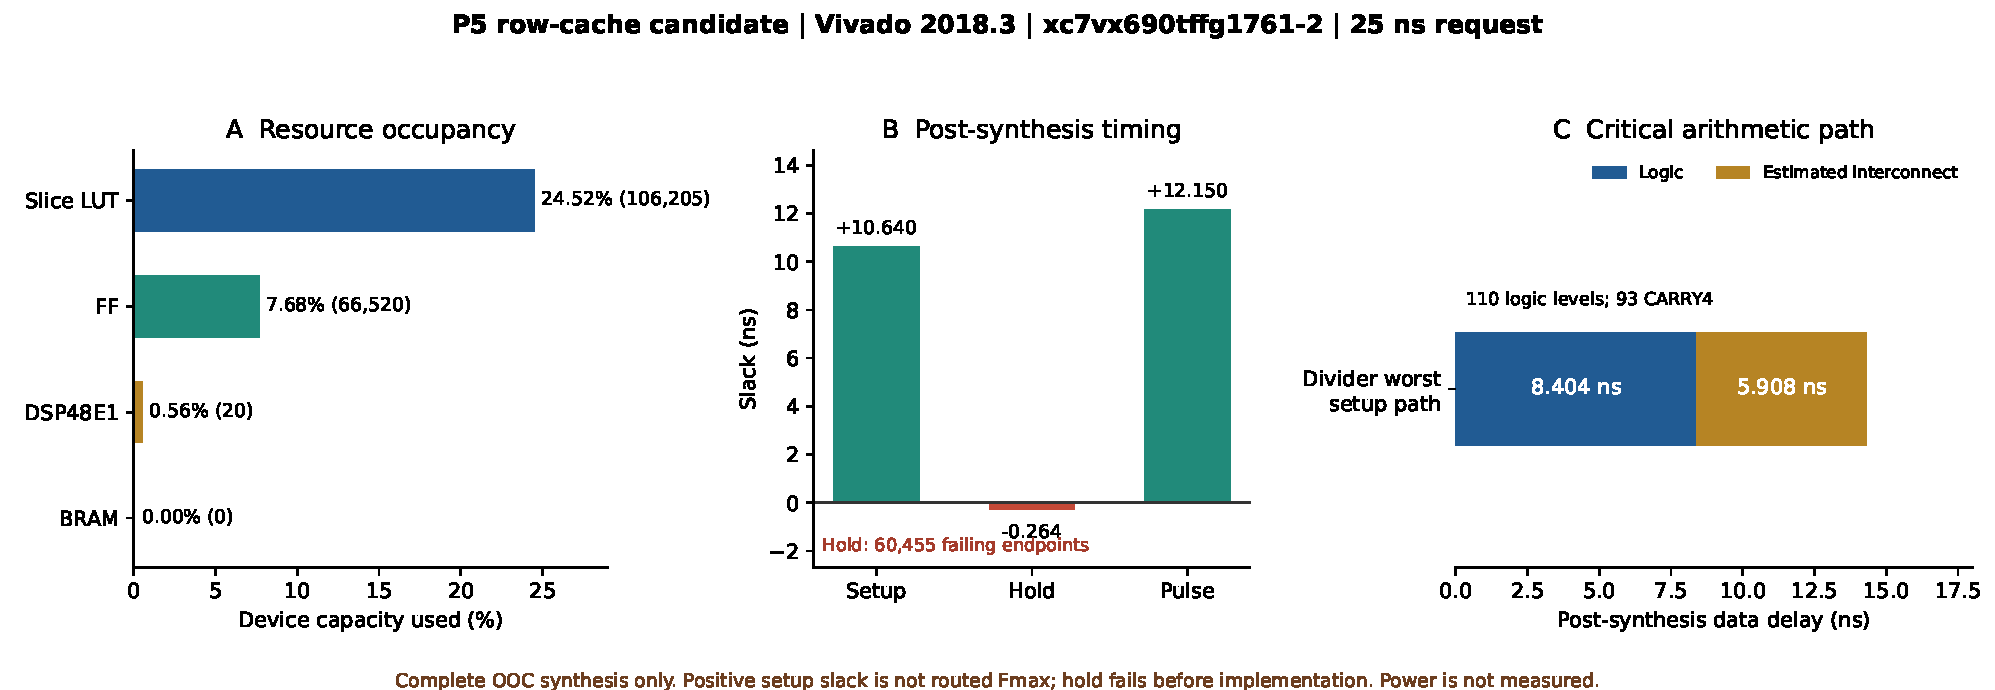
\includegraphics[width=\textwidth]{figures/cached_p5_synthesis.pdf}
\caption{当前缓存版P5的原始\code{utilization.rpt}、\code{timing_summary.rpt}和\code{timing_paths.rpt}重绘：A为器件资源占用，B将setup/hold/pulse分开，C拆出最坏除法路径的逻辑延迟与\emph{综合后估算}互连延迟。图中25\,ns为申请约束，hold负值仍然保留；脚本与来源哈希见\code{audit_figures/make_cached_p5_synth_evidence.py}及同名\code{*.sha256.json}。}
\end{figure}

最坏setup路径仍是\code{u_recon/u_div/rem_reg[0]/C}到\code{u_recon/u_div/q_reg[60]/D}：
估算数据路径14.312\,ns，110级逻辑，含93级CARRY4；该路径没有因行和缓存自动消失。
hold负裕量与未布线、无真实内部时钟缓冲的OOC状态有关，是否能由布局布线消除仍需后述BUFG实跑判定。
这一单独快照与前代P5的超时记录不能构成同约束资源收益；
也不能把此处的P5数值同P7的1.5625\,ns数据归因为缓存效果。
当前P5的\code{power_vectorless.rpt}另给出总功耗0.408\,W，其中动态0.083\,W、静态0.324\,W；
报告标明\code{Simulation Activity File=---}、置信等级Medium，并警告高扇出复位网络的活动假设可能使估算失准。
它不是活动数据标注的实测值；与下节P7的1.580\,W来自不同的周期及结构配置，不能相减作为缓存节能量。

\subsection{完整顶层综合映射后的功能见证}
为检验上述有效P5网表是否只在报告中保留面积数字、却在功能上丢失输入因果，
本轮从同一49,687,597字节DCP导出Vivado 2018.3功能网表，使用XSim直接实例化完整
\code{sar20_digital_core}。测试台仅驱动公开端口，不用\code{force}或读取内部信号；
它配置18个物理单元，逐项读回3,900次配置值，并运行三种确定性输入模式。
第一次尝试因DCP设计名为\code{checkpoint_post_synth}而非预设顶层名，在仿真前停止；
第二次尝试发现Vivado把多维端口拆成58个转义行端口，在\code{xelab}处停止。
修正\emph{测试台连接及导出流程}后的第三次运行才得到\code{FULL\_MAPPED\_FUNCTIONAL\_PASS}；
三次原始记录全部保留，不能将前两次称为功能通过。

最终运行的\code{xsim.log}明示三模式共438个输出行、7,680项协议检查和三次取消。
本地另从CSV逐行复算：每种模式146个有效sample ID，2--158之间各跳过11个，
159为取消；438个\code{code}与测试台独立期望值一致，438个\code{flags}均与期望0一致。
每种模式相邻的145对已接受样本满足
\(\Delta\texttt{clock}=16\Delta\texttt{sample\_id}\)，合计435对。
原始trace、日志及96项payload哈希见
\code{docs/evidence/20260930/vivado_cached_p5_full_mapped/}；
其中trace的SHA-256由下面两行连续拼接：
\par\noindent\code{c40ce4404bbbeae26df514be6484722}\quad
\code{682f936a626c56bd156ada9b5ae8d2073}。\par

\begin{figure}[H]\centering
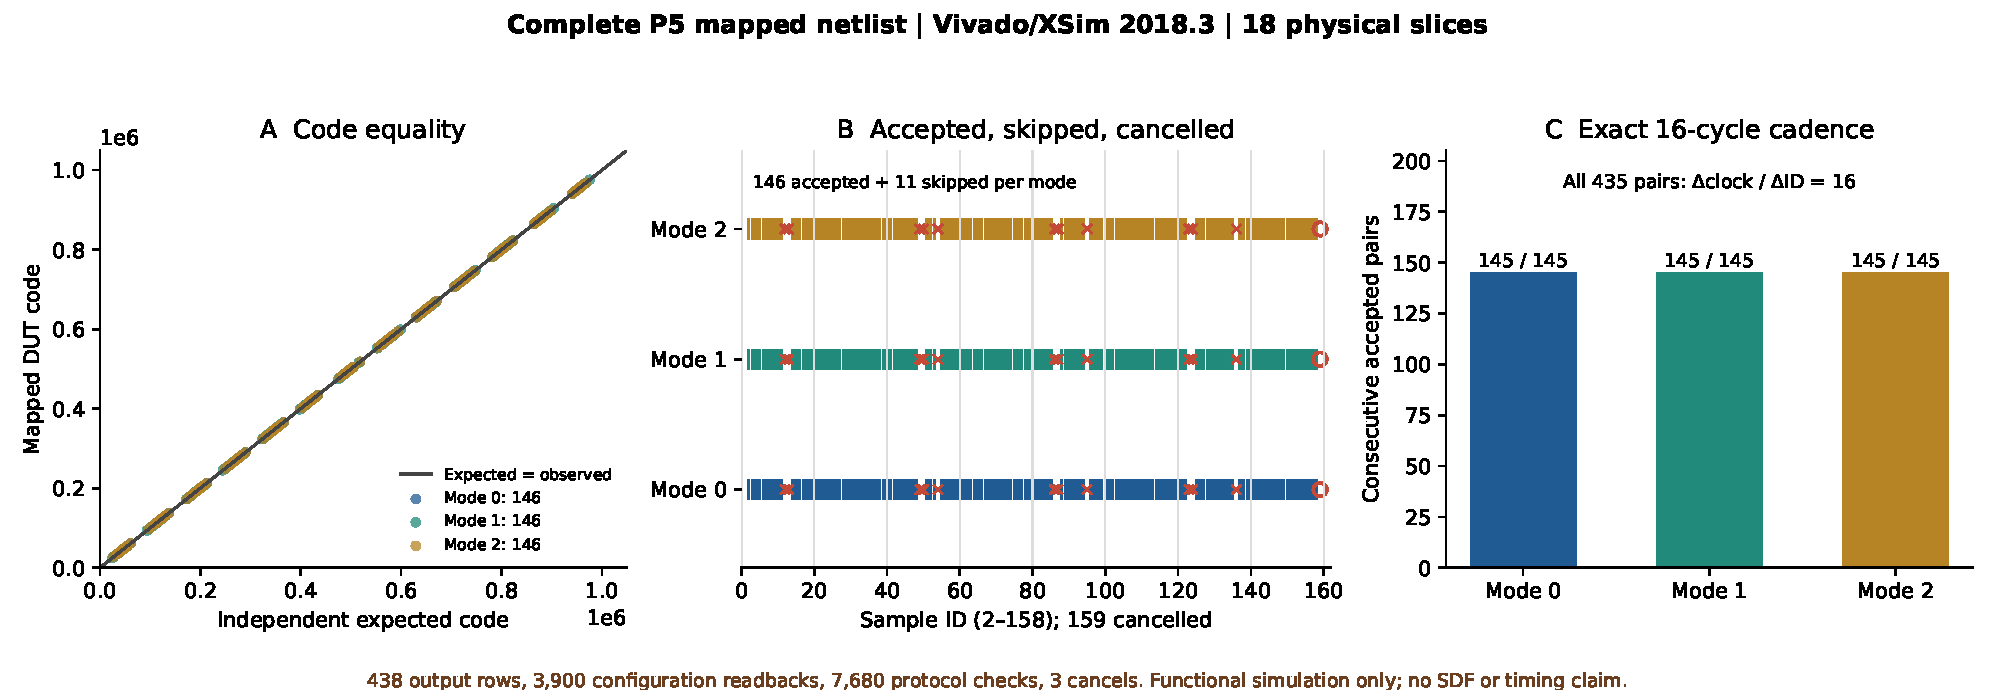
\includegraphics[width=\textwidth]{figures/mapped_p5_full_top.pdf}
\caption{完整P5顶层功能网表的实际XSim CSV：A逐点对照独立期望码，B标出每模式146个有效、11个跳过及取消样本，C检查435对相邻有效输出的16拍/样本ID节拍。原始数据和图件由\code{audit_figures/make_mapped_p5_evidence.py}及同名\code{*.sha256.json}逐项绑定。它不是SDF仿真，也不验证非零flags、内部启动延迟、模拟宏或物理时序。}
\label{fig:full-mapped-p5}
\end{figure}

这组结果把“已完整综合”进一步推进到\emph{选定刺激下的完整顶层映射功能一致}；
P5综合报告的负hold裕量仍然存在。该见证没有SDF反标，没有非零输出flag激励，
也没有检测内部重构启动延迟，因此既不是全面等价证明，也不是40\,MHz的布线结论。

\section{功耗验收不能由LUT数量替代}
前述P7归约/除法候选的原始\code{power_vectorless.rpt}给出下列模型分项。
它对应1.5625\,ns请求周期、尚未布局布线的网表，\code{Simulation Activity File}为空，
报告置信等级为Medium；这些数值是工具估计，不是芯片或FPGA板卡实测功耗。
\begin{center}
\begin{tabular}{lr}\toprule
模型分项&估计功耗/W\\\midrule
Clocks&0.664\\
Slice Logic&0.319\\
Signals&0.260\\
Dynamic合计&1.243\\
Device Static&0.337\\
Total On-Chip&1.580\\\bottomrule
\end{tabular}
\end{center}
Clocks约占该次模型动态功耗的53.4\%，说明只看LUT数量不能覆盖所有功耗来源。
这个比例也不能移用到25\,ns约束、缓存版本或布线后实现；时钟分项中的Used计数不等于独立时钟域数。
系数在运行期保持不变，并不自动证明其所有时钟网络都停止翻转；新增行和状态的开销必须一起计入。

官方\href{https://docs.amd.com/v/u/2018.3-English/ug907-vivado-power-analysis-optimization}{UG907 v2018.3，第33、78页}
说明向量无关估计依赖输入和控制信号的活动假设，FPGA的CE可用于减少无效状态更新；
这不构成对本设计的节能比例保证。本工程下一轮功耗实验应在相同器件、电压、温度、周期和实现阶段下，
分别记录配置装载、稳定16拍事务流及空闲三个工作区间，再导入各自真实活动数据。
应同时交代活动数据的时间窗口、实例匹配、未标注网络和复位占比，不能用装载期或长时间复位的低活动掩盖正常转换功耗。
若评估每样本能耗，应把稳态功耗除以实际通过的样本率，并单列装载能量，避免把不同吞吐的总瓦数直接排序。

时钟使能、操作数保持和专用时钟门控是不同层级的措施。当前RTL保留单一同步时钟，
本轮不以组合门直接改写时钟，也未完成ASIC集成时钟门控单元的映射、测试使能或时钟树验证。
若后续导入该类ASIC单元，必须重新检查门控建立/保持、复位可达性、测试模式和功能等价；
不能把FPGA的CE映射当成ASIC时钟树已经优化。面积、时序和有活动数据的功耗应分别形成证据，再判断整体PPA取舍。

\section{ASIC 目标仍需什么证据}
ASIC 的 640\,MHz 目标需要指定标准单元库、PVT、负载、时钟树、布线寄生和模拟宏接口预算。
FPGA 的 CARRY4、LUT 和 DSP48E1 与 ASIC 单元的延迟结构不同，不能按单一比例换算。
报告给出的除法分段、精确饱和商缩域和系数预聚合方案，是可以继续综合验证的结构候选；
只有在相同目标库下证明功能和约束完整，再取得有效的面积/时序/活动功耗对照，才能宣称 ASIC PPA 优势。

这一限制不妨碍本轮修复具有明确价值：已经排除了被综合器删除功能的实现方式，
使精确整数校准在 RTL 与映射见证中保持一致，并建立不会把无效网表或负时序当成成功的运行门禁。
后续每一个面积和频率数字都能追溯到相应源码、约束和原始报告，而不依赖文档作者的主观判断。


\chapter{结论}
当前代码最完整且最可检验的是\textbf{数字校准链}：物理单元权重配置、DEM/采样轨对应、Q30/Q32 整数公式、精确 floor 除法、异常与 sample ID 协同输出。当前行和缓存版本已通过22项CI RTL回归、三类lint及独立算术审计，定向最大表与替换/clear检查、两项破坏负控和P5/P6/P7结构配置检查分别保留来源；独立整数oracle、负控和真实小单元映射见证补充了不同层级的证据。P5完整顶层综合网表又通过三模式438行公开端口功能检查，但不含SDF和非零flags；历史CI与逐样本图仍按原来源保留。

首次P5基线在25\,ns下寄存器间setup为−0.280\,ns；逐行独立读选候选又因14.66\% LUT增长及拥塞等级7失败而弃用。最终共享单位读选版本通过完整22项RTL回归、三档结构检查及完整P5综合网表XSim，同约束真实BUFG布线setup为+0.946\,ns、寄存器间hold为+0.052\,ns，路由和DRC错误为0。当前40\,MHz核心在记录条件下实现，16拍节拍对应2.5\,MS/s。OOC外部hold仍为−2.278\,ns，整板接口尚未签核，ASIC 640\,MHz也未验证。综合LUT增加2.483\%，是当前时序修复的面积代价。

论文的两路交替与 RDAC 已决位隔离已到数字控制层；采样时刻、辅助充电、动态参考、RA/AZ 和比较器仍要由模拟电路和版图证明。六项专利中 US10707889B1 的跨 ADC tracking 更新尚未覆盖，但缺少证据证明它是该论文芯片必须采用的路径；应作为专利覆盖差距管理。论文披露的两端口 dither 范围扩展 2 bit 则是当前 RTL 尚未闭合的明确架构差距。下一阶段优先按已测权重归约布线路径和93.72\%权重存储FF占比优化，评估后级转换期间预计算及降低系数读取项数。二维DEM前缀算法虽有3,354,624次整数比较见证，简单叠加缓存会额外增加72,432个状态位，故尚未纳入RTL。随后实现未闭合数字架构及模拟宏接口并完成混合信号验收；ASIC 640\,MHz目标与FPGA实测可实现频率分别报告。

\appendix
\chapter{来源与复现索引}
\begin{enumerate}
\item [00] 用户提供的 ISSCC 2024 论文 PDF（文件名以 \code{[00]_A_9.3nV} 开头），第 1--3 页，尤其 Fig. 9.8.1--9.8.3。
\item [00\_1] 用户提供：\code{[00_1]ISSCC2024_ppt.pdf}，第 10--35 页为架构、参考、DEM、RA/AZ；第 36--38 页为测量结果。
\item [01] Hurrell 等，\emph{An 18 b 12.5 MS/s ADC With 93 dB SNR}，用户 PDF 第1、3、5--6页：双级多位 SAR、非易失权重修正、后级 dither 与功耗口径。
\item [02] ElShater 等，\emph{A 10-mW 16-b 15-MS/s Two-Step SAR ADC With 95-dB DR Using Dual-Deadzone Ring Amplifier}，用户 PDF 第1、7、10页：RA 结构、片上建立表征及不同采样率下的 DR/功耗。
\item [03] Li 等，\emph{A Rail-to-Rail 12 MS/s 91.3 dB SNDR 94.1 dB DR Two-Step SAR ADC With Integrated Input Buffer Using Predictive Level-Shifting}，用户 PDF 第1--3、8页：预测性输入驱动和测量条件。
\item [04] Bannon 等，\emph{An 18 b 5 MS/s SAR ADC with 100.2 dB Dynamic Range}，用户 PDF 第1--2页：三级子 ADC、残差放大、熔丝修正及不同功耗边界。
\item [05] Analog Devices，\emph{LTC2387-18 Datasheet}，用户 PDF 第1页及电气特性表：外部接口、参考与产品典型值。
\item [06] Steensgaard 等，\emph{A 24b 2MS/s SAR ADC with 0.03ppm INL and 106.3dB DR in 180nm CMOS}，用户 PDF 第1页：DEM/dither 失配整形、AZ 与 core 功耗。
\item [07] Texas Instruments，\emph{ADC358x Datasheet}，用户 PDF 第1、6页：ADC3583 型号、噪声与外部参考/双线接口功耗条件。
\item [08] Shen 等，\emph{A 16-bit 16-MS/s SAR ADC With On-Chip Calibration in 55-nm CMOS}，用户 PDF 第1、8页：片上前台位权测量、储能参考、LSB 重复与统计余差。
\item 附件身份清单：\code{audit_figures/reference_input_manifest.json} 记录 [00]、[00\_1]、[01]--[14] 共16份用户 PDF 的文件名、页数、字节数和 SHA-256；报告包不附原件。
\item [09] \url{https://patents.google.com/patent/US10516408B2/en}，claim 1 及相关图。
\item [10] \url{https://patents.google.com/patent/US10505561B2/en}，claim 1、5--11。
\item [11] \url{https://patents.google.com/patent/US10511316B2/en}，claim 1、7、8、15、20。
\item [12] \url{https://patents.google.com/patent/US10707889B1/en}，claim 1/12/23；tracking 限定必须单独核对。用户论文 PDF 第3页参考[12]印为10,797,889；按附件、题名和作者核对，交织专利为10,707,889 B1。前一号码对应另一项DLOA专利。此勘误已登记在仓库第六份外部复核文档，本文明确沿用订正号。
\item [13] \url{https://patents.google.com/patent/US10541702B1/en}，claim 1、2、6。
\item [14] \url{https://patents.google.com/patent/US10826519B1/en}，claim 1、12。
\item 仓库审查基线：PR \#4，\url{https://github.com/defineiocc02/20bit_SAR_ADC_Behaviour_Verification/pull/4}。CI run 36429986692 可从 PR 的 Checks 打开。
\item 本地独立证据包：\code{sar_adc_sim_evidence_20260928}，含报告、\code{manifest.json}、原始 CI 日志、逐样本轨迹与图。报告中的图片是原始数据可视化。
\item 旧版修复基线本地21项回归：\code{docs/evidence/20260930/final_rtl/result.json}、\code{source_manifest.json}、\code{sha256.json}，并列保存21份run log与3份lint log。
\item 旧版修复基线三参数结构回归：\code{docs/evidence/20260930/final_profiles/}，含5/6/7展开的命令、源文件摘要、逐配置manifest、延迟及协议日志。
\item 当前缓存版的真实CI原始材料：\code{docs/evidence/20260930/ci_rtl_417f/}逐项保存22份RTL测试台日志、三类严格lint及独立算术审计；\code{ci_workflow_417f/}单独保存同一head的9项工作流最终结论。两份清单均有文件SHA-256。
\item 本地独立归约验收：\code{docs/evidence/20260930/reducer_scheduler/}记录旧实现、新的列共享实现和逐单元scalar oracle在七种几何下的1,430,848次比较；\code{weight_row_cache/}另存行和装载、更替、clear、极值和两项变异负控。它们不是额外芯片样本。
\item 独立算术入口与原始负控：\code{docs/evidence/20260930/arithmetic_runner_ci/}保存两版Verilator日志、MAC/ADC2/除法/flags的正向计数及故意引入错误后的失败行；历史\code{ci_rtl_0c4a/}仍保留旧CI失败，不被后来的通过覆盖。
\item 已完成的P7完整顶层综合对照：\code{docs/evidence/20260930/vivado_complete_p7/}保留两份原始报告子集、精确源码包、日志、DCP哈希、状态和对照JSON。其1.5625\,ns约束下负WNS不代表达频，也不是当前缓存版的同约束PPA对照。
\item 前代精简P5超时记录：\code{docs/evidence/20260930/vivado_compact_p5_timeout/}保存7,200\,s时限及运行阶段，无完整DCP和资源/时序值；它是失败历史，不能填入PPA表。
\item 当前缓存P5完整顶层综合和功能网表：\code{docs/evidence/20260930/vivado_cached_p5/}保存原始报告、无驱动检查及DCP摘要；\code{vivado_cached_p5_full_mapped/}保存三次XSim尝试、最终438行trace、日志及96项文件哈希。图\ref{fig:full-mapped-p5}限定为功能证据，不代替物理时序。
\item 当前缓存P5的25\,ns实际布线失败：\code{docs/evidence/20260930/vivado_cached_p5_route_25ns_fail/}保存完整路由、DRC、setup/hold与功耗报告；\code{regreg_followup/}在同一布线DCP上按顺序引脚重算寄存器间setup/hold。图\ref{fig:p5-route-25ns}分开OOC外部端口与内部寄存器，未把负WNS归入时序通过。
\item 局部行更新候选的RTL实测：\code{docs/evidence/20260930/local_row_trial_rtl/}绑定唯一RTL内容摘要，保留官方Verilator 5.020的22项run/build日志、三类lint、P5/P6追加结构测试及57项文件哈希。图\ref{fig:local-row-profiles}显示P5/P6/P7各自15/13/11拍，不把零延迟拍数当作物理纳秒。
\item 局部行更新候选的真实EDA负证据：\code{docs/evidence/20260930/local_row_trial_synth/}保存同约束P5综合、完整DCP摘要、源码差异仅一文件的A/B比较；\code{local_row_trial_route_congestion/}保存\code{Route 35-3}拥塞等级7失败的原始日志及状态。图\ref{fig:local-row-ppa}只对比有效综合资源及路由是否完成，不存在可称为通过的最终路由时序。
\item 最终共享单位读选修复的四组完整来源：\code{docs/evidence/20260930/shared_old_trial_rtl/}、\code{shared_old_trial_synth/}、\code{shared_old_trial_route_25ns/}、\code{shared_old_trial_full_mapped/}分别绑定最终源码、同约束综合、真正寄存器间时序与完整XSim公共端口记录。图\ref{fig:shared-old-ppa}与图\ref{fig:shared-old-mapped}不继承历史失败候选的身份。
\item 后续PPA算法分析：\code{audit_figures/audit_dem_prefix_math.py}与\code{dem_prefix_math.result.json}记录独立前向物理排列、全部状态/计数、基向量和错误一维环负控；这是数学等价证据，未实现为RTL。
\item 图件来源：\code{audit_figures/}中的自写生成器及\code{*.sha256.json}核对图件、原始日志和生成脚本；仓库报告包的\code{history/}逐代保存旧图，避免把不同源码版本的曲线误合并。
\end{enumerate}
\end{document}
